\documentclass[]{report}
%% Useful packages
\usepackage[utf8]{inputenc}
\usepackage[a4paper,left=2cm,right=2cm,top=2cm,bottom=2cm]{geometry}
\usepackage{crop,graphicx,amsmath,array,color,amssymb,fancyhdr,lineno,float,booktabs}
\usepackage{flushend,stfloats,amsthm,chngpage,times,,lipsum,lastpage,parskip} 
\usepackage{calc,listings,color,wrapfig,tabularx,longtable,multirow,enumitem,commath,siunitx,ulem}
\usepackage[table,xcdraw]{xcolor}
\usepackage[font=itshape]{quoting}
%\usepackage[numbers]{natbib}
%\usepackage[subtle]{savetrees}
\usepackage[
  nottoc
  %notlot
  %notlof
]{tocbibind}

\usepackage{tikz}
\usetikzlibrary{positioning, fit, calc}   
\tikzset{block/.style={draw, thick, text width=3cm ,minimum height=1.3cm, align=center},   
line/.style={-latex}     
}

\usepackage{titlesec}

\titleformat{\chapter}[display]
{\normalfont\huge\bfseries}{\chaptertitlename\ \thechapter}{20pt}{\Huge}

% this alters "before" spacing (the second length argument) to 0
\titlespacing*{\chapter}{0pt}{0pt}{40pt}

\usepackage{hyperref}
\hypersetup{
    colorlinks=true,
    linkcolor=black,
    filecolor=teal,      
    urlcolor=teal,
    citecolor=teal,
    pdftitle={MECH0010 Topic Notes},
    pdfauthor={HD},
}

\renewcommand\bibname{References}
\usepackage{lineno}
%%%%%%%%%%%%   Header and Footer  %%%%%%%%%%%%%
\pagestyle{fancy}
\title{%
  Topic Notes}
\author{HD
}

\newcommand{\Lagr}{\mathcal{L}}

\begin{document}
\begin{titlepage}

  \newcommand{\HRule}{\rule{\linewidth}{0.5mm}} % Defines a new command for the horizontal lines, change thickness here

  %----------------------------------------------------------------------------------------
  %	LOGO SECTION
  %----------------------------------------------------------------------------------------
  \center
  
\includegraphics[width=5cm]{Title/UCL.png}\\[1cm] % Include a department/university logo - this will require the graphicx package

  %----------------------------------------------------------------------------------------

  \center % Center everything on the page

  %----------------------------------------------------------------------------------------
  %	HEADING SECTIONS
  %----------------------------------------------------------------------------------------

  \textsc{\LARGE University College London }\\[1.5cm] % Name of your university/college
  \textsc{\Large MEng Mechanical Engineering  }\\[0.5cm] % Major heading such as course name
  \textsc{\large MECH0071 Electrical Power Systems and Electrical Propulsion }\\[1.5cm] % Minor heading such as course title

  %----------------------------------------------------------------------------------------
  %	TITLE SECTION
  %----------------------------------------------------------------------------------------
  \makeatletter
  { \huge \textsc \@title}\\[1.5cm] % Title of your document


  %----------------------------------------------------------------------------------------
  %	AUTHOR SECTION
  %----------------------------------------------------------------------------------------

  \begin{minipage}{0.4\textwidth}
    \begin{flushleft} \large
      \emph{Author:}\\
      \@author % Your name
      \\[1.2em]
      %\emph{ID No:}\\
      %0101010 \\[1.2em]
    \end{flushleft}
  \end{minipage}
  ~
  \begin{minipage}{0.4\textwidth}
    \begin{flushright} \large
      \emph{Module coordinator:} \\
      Prof. Richard Bucknall \\[1.2em] % Supervisor's Name
      %\emph{Module teaching team:} \\
      %Dr. Tim Hillel\\ % second marker's name
      %Mr. Umut Lagap
    \end{flushright}
  \end{minipage}\\[2cm]
  \makeatother

  % If you don't want a supervisor, uncomment the two lines below and remove the section above
  %\Large \emph{Author:}\\
  %John \textsc{Smith}\\[3cm] % Your name

  %----------------------------------------------------------------------------------------
  %	DATE SECTION
  %----------------------------------------------------------------------------------------

  {\large \today}\\[2cm] % Date, change the \today to a set date if you want to be precise

  \vfill % Fill the rest of the page with whitespace

\end{titlepage}

\fancyhf{}
\fancyhead[L]{MECH0010}
\fancyfoot[L]{HD}
\fancyfoot[R]{ \bf\thepage\ \rm }%

\fancypagestyle{plain}{%
  \fancyhf{}%
  \fancyfoot[L]{HD}
  \fancyfoot[R]{ \bf\thepage\ \rm }%
  \renewcommand{\headrulewidth}{0pt}% Line at the header invisible
  \renewcommand{\footrulewidth}{0pt}% Line at the footer visible
}

\newpage
\tableofcontents
\newpage
\listoffigures
\listoftables
\newpage
\part{Control}
\chapter{Introduction to Control Systems}
A \textbf{control system} is a mechanism which alters the future state of a particular system. \textbf{Control theory} is the method of selecting appropriate inputs. Control theory usually concerns dynamic behaviour of physical systems - the goal is to design a controller which leads to the system exhibiting the desired behaviour. Control systems have a large range of applications throughout engineering such as autopilot systems for ships and aircraft, radar tracking, robotics, machinery plant control and machine tools.
\subsection*{Methodology}
\begin{itemize}
  \item \textbf{Modelling} - Mathematical model of a system or "transfer function." Comes from detailed analysis of a system and often involves simplifications
  \item \textbf{Prediction} - The model is used to predict the behaviour of the system for a range of parameters and expected excitations
  \item \textbf{Design} - Design a controller which achieves its operating objectives and test it on the model
  \item \textbf{Test} - Here, theory is taken into reality and we compare our model to the physical hardware. Testing of the validity of our assumptions also takes place
  \item \textbf{Iterate} - Improve controller design through updated models
\end{itemize}
\section{Open loop control}
In an \textbf{open loop} control system, the input to the system is not dependant on any previous outputs. The output of the system is not being observed to confirm whether the desired output has been achieved.
\begin{figure}[H]
  \centering
  \includegraphics[width = 0.8\textwidth]{./img/openloopcontrol.png}
\end{figure}
These control systems are simple and low cost. They are used in systems where feedback is not important. For example, a washing machine runs for 90 minutes, regardless of whether the clothes are dry after 60 minutes.
\subsection*{3D Printer example}
Consider the stepper motors used to move the print head in x and y with belt and pulley system. Here, open loop control is used because the stepper motors are simple to control and have a relationship between input and output. For example, consider a stepper motor which moves 0.2\si{\milli\m} each step (S) for an integer number of steps.
\begin{verbatim}
  Plant model: X = 0.2 S
  Control strategy: S = X/0.2
\end{verbatim}
\begin{figure}[H]
  \centering
  \includegraphics[width = 0.8\textwidth]{./img/controlstrat3dprinter.png}
\end{figure}
Implementing such a controller could be done with the following pseudocode:
\begin{verbatim}
  Function MovePrintHeadX(Input_mm)
  //convert to number of steps needed
  Steps_S = Input_mm / 0.2
  //send step command to motor
  Stepper.step(Steps_S)
\end{verbatim}
However, the assumption used to model our system is only valid if the stepper motors is within its specification i.e. friction, load, temperature, power are all nominal. As stated before, the system does not observe if the steps were successful or not.
\section{Closed loop control}
By observing the output and comparing it against your desired output, it is possible to update the input to the system. The observed output is called the \textbf{feedback signal}.
\begin{figure}[H]
  \centering
  \includegraphics[width = 0.8\textwidth]{./img/closedloopcontrol.png}
\end{figure}
The difference between the desired output and the feedback signal is known as the \textbf{error signal}. This is the signal that the controller uses. Feedback signals allow powerful controllers to be designed.

Taking our 3D printer for example, we can add a position sensor on the x-axis.
\begin{figure}[H]
  \centering
  \includegraphics[width = 0.8\textwidth]{./img/controlstrat3dprinterclosed.png}
\end{figure}
The pseudocode for this system could look like this
\begin{verbatim}
  while
    // get measurement of position
    measured_value_mm = Sensor.getValue
    // calc error signal
    error_mm = setpoint_mm - measure_value_mm
    // convert to steps
    Steps_S - error_mm / 0.2
    // send step command to motor
    Stepper.Step(Steps_S)
  end
\end{verbatim}
We must consider whether this extra complexity is required or necessary in our system. Closed loop systems are not a magic bullet; they require careful modelling to predict system behaviour and a considered choice of parameters to prevent the system becoming unstable.
\section{Block diagram representation of control loops}
\begin{figure}[H]
  \centering
  \includegraphics[width = 0.8\textwidth]{./img/blockdiagram1.png}
\end{figure}
Control systems are often represented by block diagrams which show the information flow.
\begin{figure}[H]
  \centering
  \includegraphics[width = 0.8\textwidth]{./img/blockdiagram2.png}
\end{figure}
\textbf{Flow path} indicates the direction of data flow (from left to right). Values are maintained at a branch.
\begin{figure}[H]
  \centering
  \includegraphics[width = 0.5\textwidth]{./img/flowpath.png}
  \caption{Flow path}
\end{figure}
\textbf{Function block}. The functions acts on the input to to produce the output. $x_{out} = f(x_{in})$
\begin{figure}[H]
  \centering
  \includegraphics[width = 0.5\textwidth]{./img/functionblock.png}
  \caption{Function block}
\end{figure}
\textbf{Comparator}. The signals $\theta_1$ and $\theta_2$ are compared according to the signs (+ or -) and the result is $\theta_3$. They \textbf{must} have the same units. In this case $+\theta_1 - \theta_2 = \theta_3$.
\begin{figure}[H]
  \centering
  \includegraphics[width = 0.5\textwidth]{./img/comparator.png}
  \caption{Comparator}
\end{figure}
\begin{figure}[H]
  \centering
  \includegraphics[width = 0.8\textwidth]{./img/blockdiagram3.png}
\end{figure}
\section{Basic definitions/concepts}
The following definitions are based on the standards of the IEEE (Institute of Electrical and Electronics Engineers)
\begin{itemize}
  \item A \textbf{system} is an arrangement, set or collection of components connected or related in such a manner as to form an entirety or whole.
  \item A \textbf{control system} is an arrangement of physical components connected or related in such a manner as to command, direct or regulate itself or another system. The components act together to perform a function not possible with any of the individual parts.
  \item The \textbf{input} is the stimulus or excitation applied to a system usually in order to produce a specified response.
  \item The \textbf{output} is the actual response obtained.
  \item An \textbf{open loop control system} is one in which the input is independent of the output.
  \item A \textbf{closed loop control system} is one in which the input is somehow dependent on the output.
  \item \textbf{Error signal} (or \textbf{actuating signal}) is the difference between the reference input and the feedback, in closed loop control systems it is this signal which is sent to the plant not the reference signal.
\end{itemize}
\section{Notation}
Large complex systems can be broken down into interconnected smaller ones and reduced further into a number of blocks.
\begin{figure}[H]
  \centering
  \includegraphics[width = 0.8\textwidth]{./img/quadcopterexampleblock.png}
  \caption{A quadcopter with lots of PID controllers running in parallel. Each colour represents a control loop for position, altitude, yaw etc.}
\end{figure}
Complex systems can be abstracted to a signal block if the behaviour can be adequately modelled. Consider modelling the stepper motor from the 3D printer, in reality a complex device, as a single block. This is analogous to representing a complex op-amp circuit as a single unit.
\begin{figure}[H]
  \centering
  \includegraphics[width = 0.8\textwidth]{./img/blockdiagram4.png}
\end{figure}
\section{Control system design process}
\begin{figure}
  \centering
  \includegraphics[width = 0.8\textwidth]{./img/controlstrat3dprinterclosed.PNG}
\end{figure}
\begin{enumerate}
  \item Establish control goals
  \item Identify the variables to control
  \item Write the specifications for the variables
  \item Establish the system configuration and identify the actuators
  \item Obtain a model of the process, the actuator and the sensor
  \item Describe a controller and select the parameters to be adjusted
  \item Optimise the parameters and analyse the performance
\end{enumerate}
\section{Summary}
\begin{itemize}
  \item Control systems are interconnected components which are configured to provide a desired response.
  \item Two broad categories of control systems: open loop (no feedback of output) and closed loop (feedback signal).
  \item Successful design of the controller requires consideration of the design goals, definition of the specifications, system definition, modelling and subsequent analysis. Controller design is an iterative process.
\end{itemize}
\section{Tutorial}
\subsection*{3D printer design choice}
\subsubsection*{The positioning of the print head is in open loop. Considering the comparative advantages of open and closed loop control, what would have lead the designers to make this choice?}
Open loop control is used where the observation of the output is not necessary/relevant to the control of the system. Considering the accuracies required for 3D printing, which is around $\pm 0.05 \si{\milli\m}$, we need to make sure that our print head moves to distances within this tolerance, otherwise our prints will be warped and misshaped. We must also consider that in an open system, small errors may lead to large errors over a certain period of operation, despite the print head moving distances within tolerance. There are also external factors affecting the belt and pulley system of the print head e.g. heat, dust, friction, load. These must all be within specification for the system to work properly.

Stepper motors are simple electronic components and can be manufactured to have a relationship between input and output. Hence, the need to observe whether the print head has moved a certain distance may be inconsequential. In applications where an extremely accurate print is required, a closed loop system would allow for a self calibrating system, which could allow the printer to work in different operational environments without the need to recalibrate or change components. However, this adds complexity to the controller and requires additional components to be added to the controller, increasing cost.
\subsubsection*{How might the designers overcome the problems mentioned without closed loop control?}
Maintenance of the components in the system is important to make sure that everything is in the correct working order. When everything is kept clean and within the specification that the system is designed to work in, the controller will be able to work optimally. For example, calibrating the "0" position of the print head after cleaning the belts and pulleys from dust.

The designers may also implement a calibration operation into the controller before each phase. This may include implementing a "0" point into the hardware of the rails that the print head is attached to. The controller would move the print head to this position simply by moving the maximum distance left and down. Using this as a reference for each print would eliminate systematic distance errors.
\subsection*{Washing machine}
\subsubsection*{Think of the control loops inside are they open or closed loop? Why? What could the sensors be?}
Let us consider the possible subsystems inside a washing machine.
\begin{itemize}
  \item Timer - controls how long the washing machine operates. Open loop system. We only need a simple timing circuit with a minimum accuracy of around $\pm 1 \si{\minute}$. Even if the washing machine runs for 85 minutes instead of 90 (some degree of inaccuracy), this is insignificant.
  \item Motor - this is to spin the tub. Open loop system. Motors are simple electronic components with a relationship between input and output. An error signal provides no useful information for the operation of the motor.
  \item Temperature control - controls how hot or cold the water in the washing machine is. Open loop system. Most washing machines simply have a hot water connection for hot water and cold water. A solenoid valve can control the proportion of hot water to cold water that enters the tub. For washing machines with a heating element, the amount of power put through the coil will determine the final temperature of the water (relationship between input and output is known). Adding a thermistor to measure the output water temperature may be possible but ultimately unnecessary as the tolerance for the temperature can be quite high ($\pm 5 \si{\celsius}$)
  \item Water valve control - controls how much water enters and leaves the drum. Closed loop control. The level of water in the drum needs to only be measured when the drum is full of water. Knowing the level of water at any given moment is unnecessary, thus using a simple pressure switch, will be sufficient in letting the controller know that the tub has reached capacity and close the input valve. After a set amount of time, the drain valve may open and since the amount of water in the tub when it is full is known, the drain time can simply be calculated as a function of its volume. This means that we do not need to check whether the water has drained from the tub.
\end{itemize}
\chapter{Modelling Linear Systems}
Previously, we have considered systems in the general sense, with a generic function block approach.
\begin{figure}[H]
  \centering
  \includegraphics[width = 0.8\textwidth]{./img/blockdiagram5.png}
\end{figure}
Now we will investigate how we model physical systems and obtain the function block $F(x)$ for electrical and mechanical components.
\section{Linear Term Invariant (LTI) systems}
The focus of this course and indeed much of control theory itself focuses on modelling physical systems as \textbf{linear} and \textbf{time invariant}. LTI systems have three key properties:
\begin{itemize}
  \item Obey principle of superposition
  \item Homogeneity
  \item Time invariance
\end{itemize}
\subsection{Superposition}
If input $x_1(t)$ produces output $y_1(t)$ and input $x_2(t)$ produces $y_2(t)$, then input $x_1(t) + x_2(t)$ produces output $y_1(t) + y_2(t)$
\begin{figure}[H]
  \centering
  \includegraphics[width = 0.8\textwidth]{./img/blockdiagram6.png}
\end{figure}
Say for a system which doubles the input $F(x) = 2x$
\begin{figure}[H]
  \centering
  \includegraphics[width = 0.8\textwidth]{./img/graphs1.png}
\end{figure}
\subsection{Homogeneity}
If the input to the system $x(t)$ is scaled by a magnitude scale factor $A$, then the output $y(t)$ is also scaled by the same factor.
\begin{figure}[H]
  \centering
  \includegraphics[width = 0.8\textwidth]{./img/blockdiagram7.png}
\end{figure}
For example, consider a system which generates a sine wave at a given amplitude, with a set frequency:
\begin{figure}[H]
  \centering
  \includegraphics[width = 0.8\textwidth]{./img/graphs2.png}
\end{figure}
\subsection{Time invariance}
If input is applied at time $t=0$ or $T \ \si{\second}$ from now, the output is identical with the exception of a delay of $T \ \si{\second}$.
\begin{figure}[H]
  \centering
  \includegraphics[width = 0.8\textwidth]{./img/blockdiagram8.png}
\end{figure}
\subsection*{Are these models suitable for physical systems?}
These three requirements, whilst simple, are so stringent that \textbf{almost no physical LTI system truly exists}. Consider a car engine - the performance deteriorates over time, to stretch it further, would you expect a system to give the same output after a time delay $T$ of 10 years? Even simple systems such as a resistor in an electrical circuit have non-linearities - a scaling factor $A$ could be chosen for $x(t)$ which would mean too much current flows and the resistor melts.

Most practical systems are not linear, but often we can assume they behave linearly \textbf{under certain conditions/assumptions}. Linear systems are \textbf{much} easier to solve! There are \textbf{analytic} solutions with standard tools used solve the equations. Whereas for non-linear problems it is often necessary to solve them numerically.
\subsection{Linearisation: Example 1}
For a simple system such as a spring, across all possible compressions or extensions the response is non-linear:
\begin{equation}
  F = -kX
\end{equation}
Hookes law is only a linear approximation of the true response. However, if we choose the operating range of the spring correctly, the response is within the linear region. This approximation is \textbf{valid}.
\subsubsection{Linearisation: Example 2}
Similarly an op-amp has a \textbf{linear region} where the output signals are between supple voltages $V_S$
\begin{figure}[H]
  \centering
  \includegraphics[width = 0.8\textwidth]{./img/graphs4.png}
\end{figure}
Keep signals within these regions and the linear assumption holds:
\begin{figure}[H]
  \centering
  \includegraphics[width = 0.8\textwidth]{./img/blockdiagram9.png}
\end{figure}
Add LTI example
\section{Dynamic systems - Laplace Transform}
\subsection{Dynamic systems as ODEs}
Ideal systems would respond \textbf{instantaneously} to inputs, however real world systems require some time to adjust to changes and are thus known as \textbf{dynamic systems} as the output changes over time.
\begin{figure}[H]
  \centering
  \includegraphics[width = 0.8\textwidth]{./img/graphs5.png}
\end{figure}
As we are intersected in describing something that \textbf{changes} with time, it is useful to express the function block of the system $F(t)$ as an ordinary differential equation (ODE).
\begin{figure}[H]
  \centering
  \includegraphics[width = 0.8\textwidth]{./img/blockdiagram10.png}
\end{figure}
\begin{equation}
  \frac{\dif^n y}{\dif t^n} + a_{n-1}\frac{\dif^{n-1}y}{\dif t^{n-1}} + ... + a_2 \frac{\dif^2y}{\dif t^2} + a_1 \frac{\dif y}{\dif t} + a_0 = bx
\end{equation}
\begin{itemize}
  \item $x$ is input function or forcing function
  \item $y$ is output
  \item $n$ is \textbf{order} of the ODE
  \item $a_0...$ are coefficients. These \textbf{completely characterise the system}
\end{itemize}
\subsection{Laplace Transforms}
Because of our \textbf{linear assumptions} we can use Laplace transforms to simplify solving the ODEs. The Laplace transforms of a signal (function) $x$ is the function $X = \mathcal{L} (x)$ defined by
\begin{equation}
  X(s) = \int_{0^-}^\infty x(t) e^{-st} \dif t
\end{equation}
For those $s \in \textbf{C}$ for which the integral makes sense.
\begin{itemize}
  \item $X$ is a complex-valued function of complex numbers
  \item $s$ is called the (complex) \textbf{frequency variable} with units \si{\per\second}, $t$ is called the \textbf{time variable} (in sec); $st$ is unitless
  \item $s = \sigma + j \omega$
\end{itemize}
As we shall see:
\begin{itemize}
  \item Differential operators are replaced with algebraic variables
  \item Algebraic equations are much easier to manipulate \& solve
  \item Standard forms exist for many physical systems
\end{itemize}
\subsubsection{Laplace Transforms: Example 1}
Let's fine Laplace transform $x(t) = e^t$:
\begin{gather}
  X(e^t) = \int_{0^-}^\infty e^t e^{-st} \dif t\\
  X(e^t) = \int_{0^-}^\infty e^{(1-s)t} \dif t\\
  X{e^t} = \left. \frac{1}{1-s}e^{(1-s)t}\right|_{0^-}^\infty \\
  X(e^t) = \frac{1}{1-s} \times 0 - \frac{1}{1-s} \times 1 = \frac{1}{s-1}
\end{gather}
\subsubsection{Laplace Transforms: Example 2}
Constant or \textbf{unit step} $x(t) =1$ (for $t \geq 0$)
\begin{gather}
  X(s) = \int_{0^-}^{\infty} 1 e^{-st}\dif t\\
  X(s) = \int = \left. -\frac{1}{s} e^{-st} \right|_{0^-}^\infty\\
  X(s) = - \frac{1}{s} \times 0 - (- \frac{1}{s}) \times 1 = \frac{1}{s}
\end{gather}
\subsubsection{Laplace Transforms: Example 3}
\textbf{Sinusoid:} first express $x(t) = \cos{(\omega t)}$ as:
\begin{gather}
  x(t) = \frac{1}{2} e^{i \omega t} + \frac{1}{2} e^{-i \omega t} \textrm{ (Euler's formula)}\\
  X(s) = \int_{0^-}^\infty e^{-st} \left( \frac{1}{2} e^{i \omega t} + \frac{1}{2} e^{-i \omega t} \right) \dif t\\
  X(s) = \frac{1}{2} \int_{0^-}^\infty e^{(-s + i \omega)t}\dif t + \frac{1}{2} \int_{0^-}^\infty e^{(-s - i \omega)t} \dif t\\
  X(s) = \frac{1}{2} \frac{1}{s - i \omega} + \frac{1}{2} \frac{1}{s + i \omega} = \frac{s}{s^s + \omega^s}
\end{gather}
You can look up these transforms in a table. The Laplace variable, s, can be considered to represent the differential operator (very useful for control engineering):
\begin{gather}
  s \equiv \frac{\dif}{\dif t}\\
  \frac{1}{s} \equiv \int_{0^-}^\infty \dif t
\end{gather}
Laplace transform of time derivative $\frac{\dif x}{\dif t}$:
\begin{equation}
  L \left\{ \frac{\dif x}{\dif t} \right\} = \int_{0^-}^\infty \frac{\dif x}{\dif t} e^{-st} \dif t
\end{equation}
Integrating by parts
\begin{equation}
  L \left\{ \frac{\dif x}{\dif t} \right\} = s \int_{0^-}^\infty x(t) e^{-st} \dif t + \left[ x(t)e^{-st} \right]_{0^-}^\infty
\end{equation}
The initial condition $x(0^-)$ is often zero in practice
\begin{equation}
  L \left\{ \frac{\dif x}{\dif t} \right\} = sX(s) - x(0^-) = sX(s)
\end{equation}
We can substitute this result to solve higher order derivatives:
\begin{gather}
  L\left\{ \frac{\dif^2 x}{\dif t^2} \right\} = sL\left\{ \frac{\dif x}{\dif t} \right\} - \frac{dif x}{\dif t} (0^-)\\
  L\left\{ \frac{\dif^2 x}{\dif t^2} \right\} = s^2 X(s) - sx(0^-) - \frac{\dif X}{\dif t} (0^-) = s^2 X(s)
\end{gather}
So more generally, with all initial conditions set to zero:
\begin{equation}
  L\left\{ \frac{d^n x}{dt^n} \right\} = s^n X(s)
\end{equation}
\subsection{Transfer Functions}
After we have taken the Laplace transform of the differential equation of a system, it's useful to rearrange to give the system \textbf{output} as the product of the system \textbf{input} and the system \textbf{transfer function}.
\begin{figure}[H]
  \centering
  \includegraphics[width = 0.8 \textwidth]{./img/blockdiagram11.png}
\end{figure}
The transfer function of a linear system is defined as the \textbf{ratio} of the Laplace transform of the output variable to the Laplace transform of the input variable, with all the initial conditions assumed to be zero.
\subsection{Transfer Functions of Mechanical Components}
\subsubsection{Spring}
Convention is input force, output displacement. Balance \textbf{forces}
\begin{figure}[H]
  \centering
  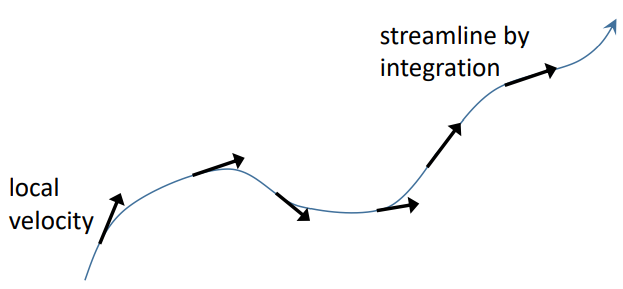
\includegraphics[width = 0.8 \textwidth]{./img/diagram1.png}
\end{figure}
Time domain equation (Hooke's Law):
\begin{equation}
  f(x) - kx
\end{equation}
$k$ is stiffness in \si{\newton\per\meter}. Laplace domain equation:
\begin{equation}
  F(s) = kX(s)
\end{equation}
Transfer function:
\begin{equation}
  G(s) = \frac{X(s)}{F(s)} = \frac{1}{k}
\end{equation}
\begin{figure}[H]
  \centering
  \includegraphics[width = 0.5\textwidth]{./img/blockdiagram12.png}
\end{figure}
\subsubsection{Mass}
Inertial load - mass
\begin{figure}[H]
  \centering
  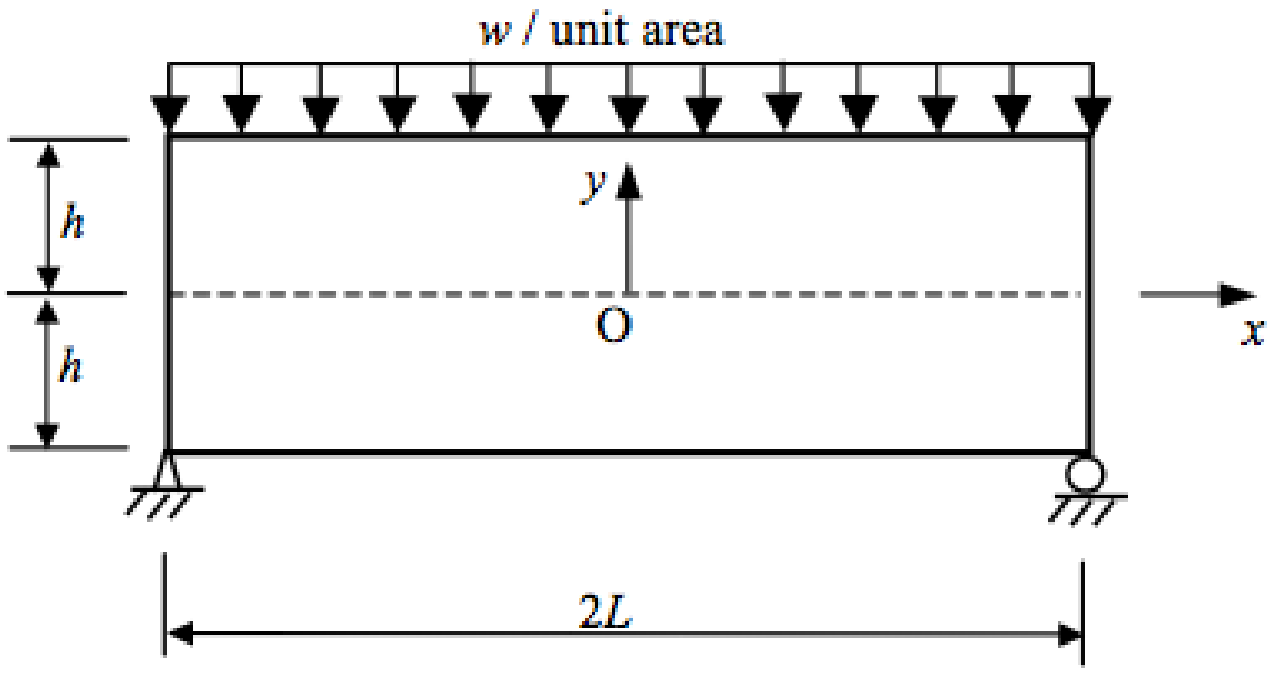
\includegraphics[width = 0.3\textwidth]{./img/diagram2.png}
\end{figure}
Time domain equation from Newton's 2nd law of motion
\begin{equation}
  f(t) = m \frac{\dif^2x(t)}{dt^2}
\end{equation}
Laplace domain equation
\begin{equation}
  F(s) = ms^2 X(s)
\end{equation}
Transfer function
\begin{equation}
  \frac{X(s)}{F(s)} = \frac{1}{ms^2}
\end{equation}
\begin{figure}[H]
  \centering
  \includegraphics[width = 0.5\textwidth]{./img/blockdiagram13.png}
\end{figure}
\subsubsection{Damper}
Below is a dashpot - a viscous damper. They resist motion through friction. The damping coefficient is in terms of $c$ with units \si{\newton\per\meter\per\second}. Time domain equation:
\begin{equation}
  f(x) = x\frac{\dif x }{\dif t} = csx
\end{equation}
Laplace domain equation:
\begin{equation}
  F(s) = csX(s)
\end{equation}
Transfer function
\begin{equation}
  \frac{X(s)}{F(s)} = \frac{1}{cs}
\end{equation}
\begin{figure}[H]
  \centering
  \includegraphics[width = 0.6\textwidth]{./img/blockdiagram14.png}
\end{figure}
\subsection{Combining components}
\subsubsection{Springs}
Springs in parallel
\begin{gather}
  k' - k_1 + k_2\\
  G(s) = \frac{X(s)}{F(s)} = \frac{1}{k'}
\end{gather}
Springs in series
\begin{gather}
  \frac{1}{k'} = \frac{1}{k_1} + \frac{1}{k_2}\\
  G(s) = \frac{X(s)}{F(s)} = \frac{1}{k'}
\end{gather}
\begin{figure}[H]
  \centering
  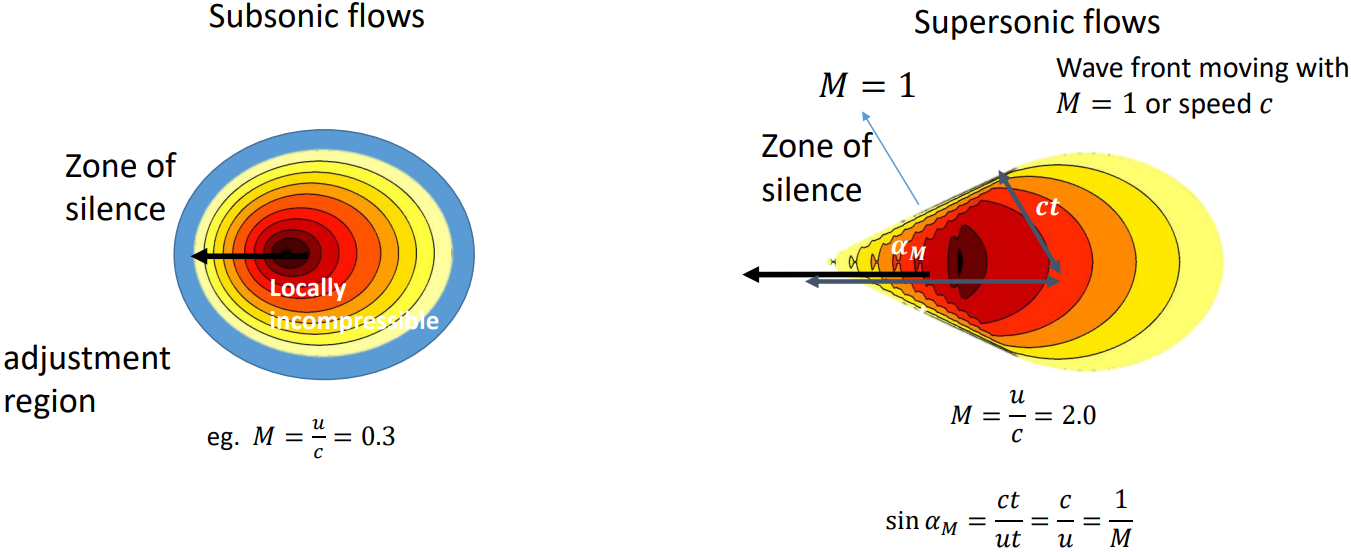
\includegraphics[width = 0.6\textwidth]{./img/diagram4.png}
\end{figure}
\begin{figure}[H]
  \centering
  \includegraphics[width = 0.6 \textwidth]{./img/blockdiagram15.png}
\end{figure}
Dashpots behave in a similar way to springs. Parallel:
\begin{equation}
  c' = c_1 + c_2
\end{equation}
and in series:
\begin{equation}
  \frac{1}{c'} = \frac{1}{c_1} + \frac{1}{c_2}
\end{equation}
\subsubsection{Resistor}
Convention is input voltage, output current. Balance voltages.
Ohms law is $V=IR$. Time domain:
\begin{equation}
  v(t) = i(t)R
\end{equation}
Laplace domain:
\begin{equation}
  V(s) = I(s)R
\end{equation}
Transfer function:
\begin{equation}
  G(s) = \frac{I(s)}{V(s)} = \frac{1}{R}
\end{equation}
\begin{figure}[H]
  \centering
  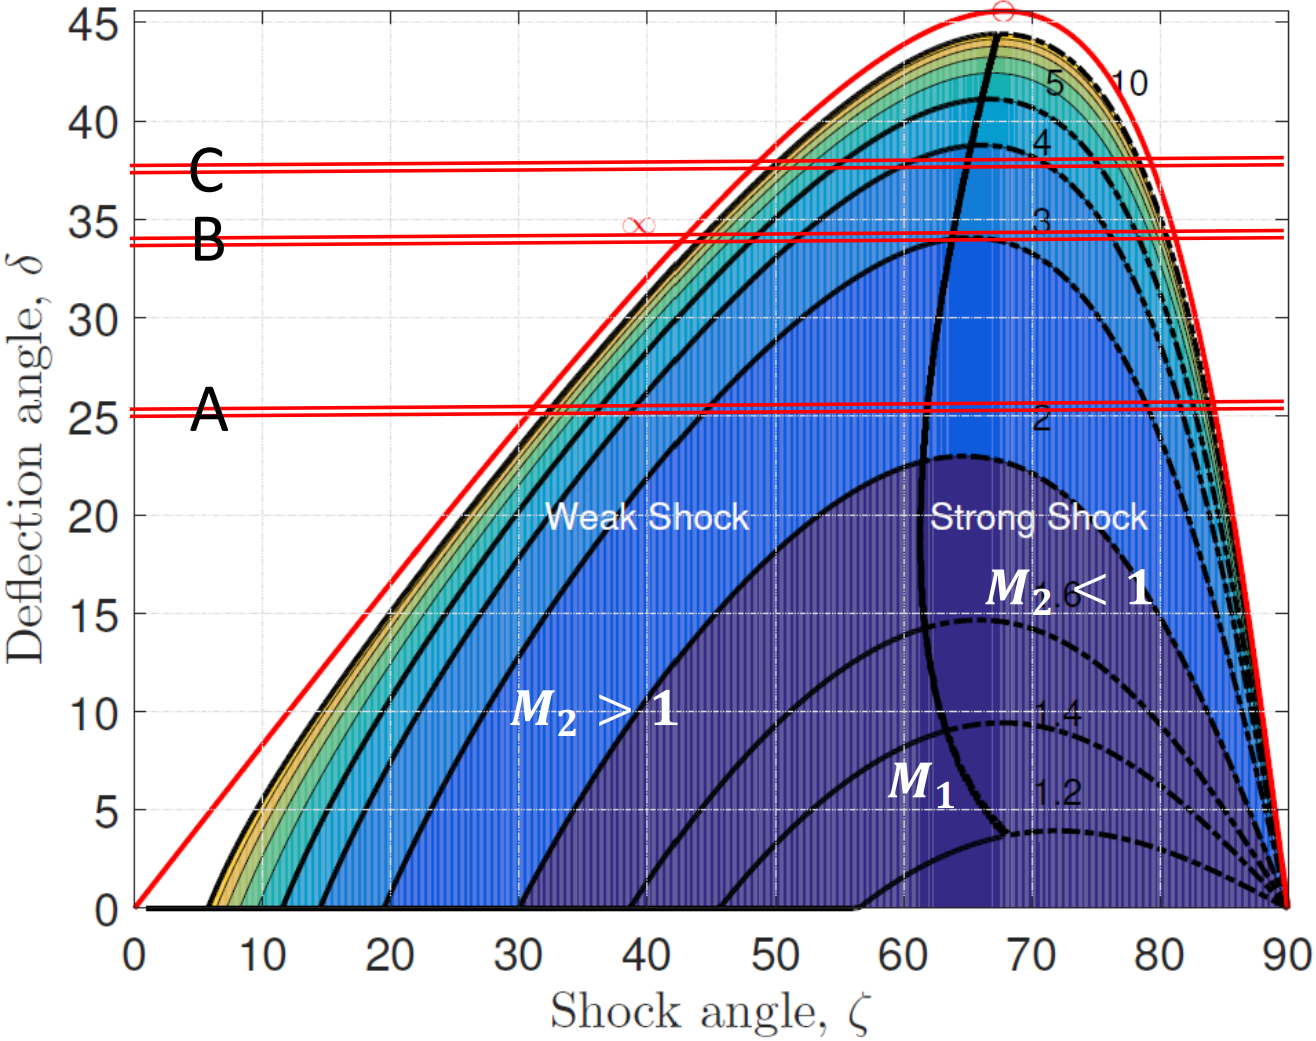
\includegraphics[width = 0.5\textwidth]{./img/diagram5.png}
\end{figure}
\begin{figure}[H]
  \centering
  \includegraphics[width = 0.5\textwidth]{./img/blockdiagram16.png}
\end{figure}
\subsubsection{Capacitor}
Either definition of current/voltage relationship gives same result. Time domain:
\begin{gather}
  i(t) = C\frac{\dif v}{\dif t}\\
  v(t) = \frac{1}{C}\int i(t) \dif t
\end{gather}
Laplace domain:
\begin{gather}
  I(s) = CsV(s)\\
  V(s) = \frac{1}{C} \frac{1}{s} I(s)
\end{gather}
Transfer function:
\begin{equation}
  G(s) = \frac{I(s)}{V(s)} = Cs
\end{equation}
\begin{figure}[H]
  \centering
  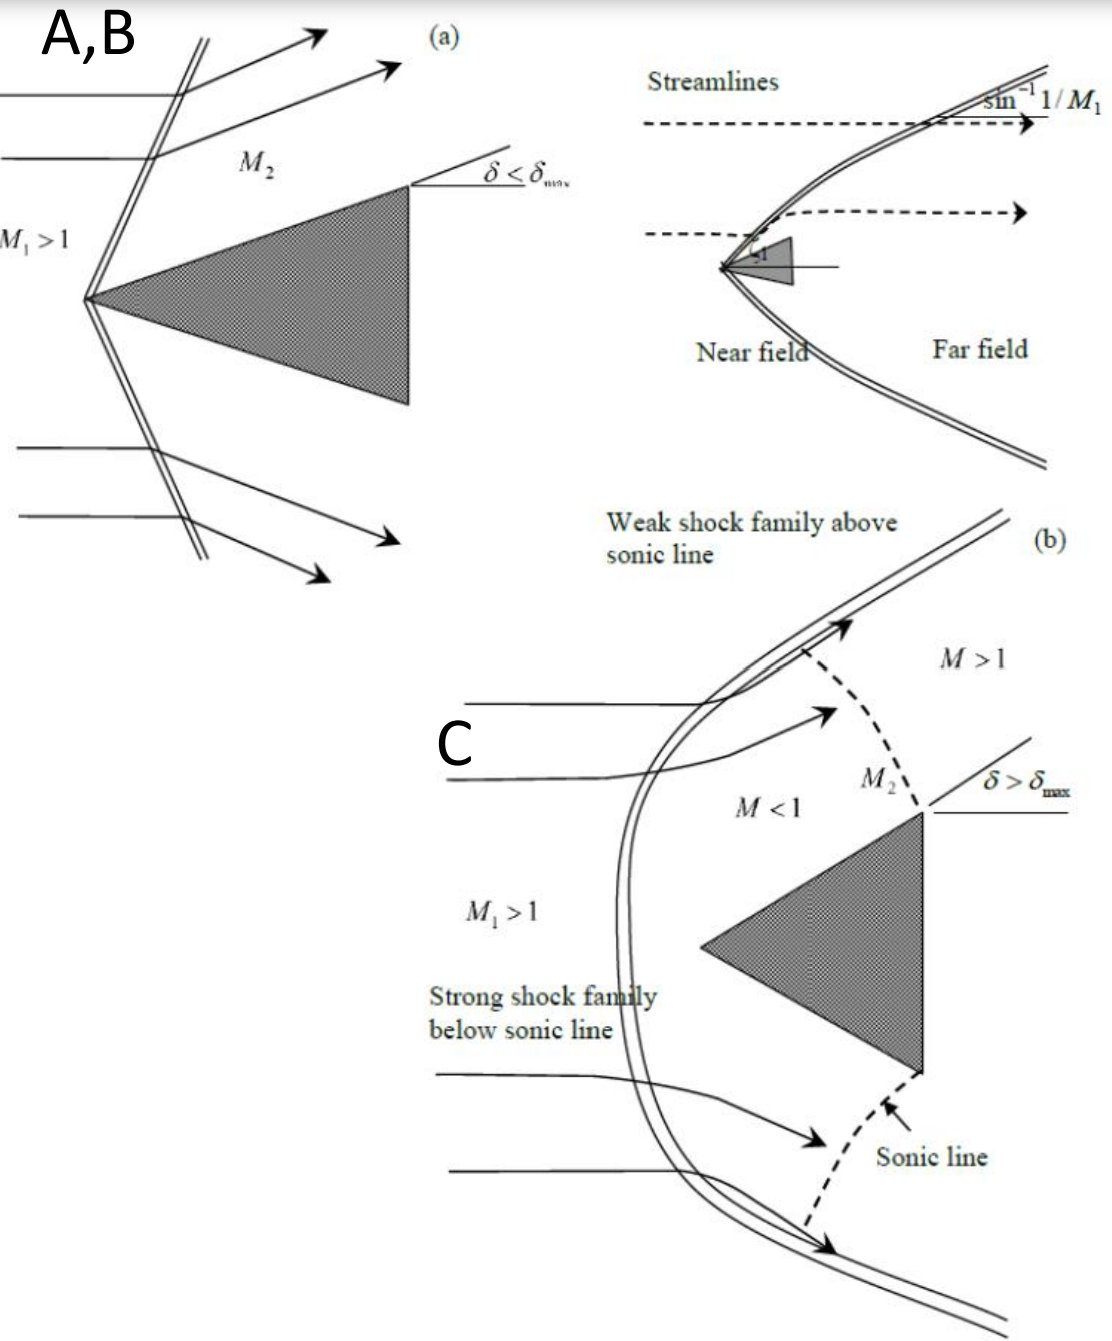
\includegraphics[width = 0.5\textwidth]{./img/diagram6.png}
\end{figure}
\begin{figure}[H]
  \centering
  \includegraphics[width = 0.5\textwidth]{./img/blockdiagram17.png}
\end{figure}
\subsubsection{Inductor}
An inductor resists changes of current by generating a voltage in opposition via magnetic induction. From Faraday's Law:
\begin{equation}
  v(t) = L \frac{\dif i}{\dif t}
\end{equation}
Laplace domain
\begin{equation}
  V(s) = LsI(s)
\end{equation}
Transfer function:
\begin{equation}
  G(s) = \frac{I(s)}{V(s)} = \frac{1}{Ls}
\end{equation}
\begin{figure}[H]
  \centering
  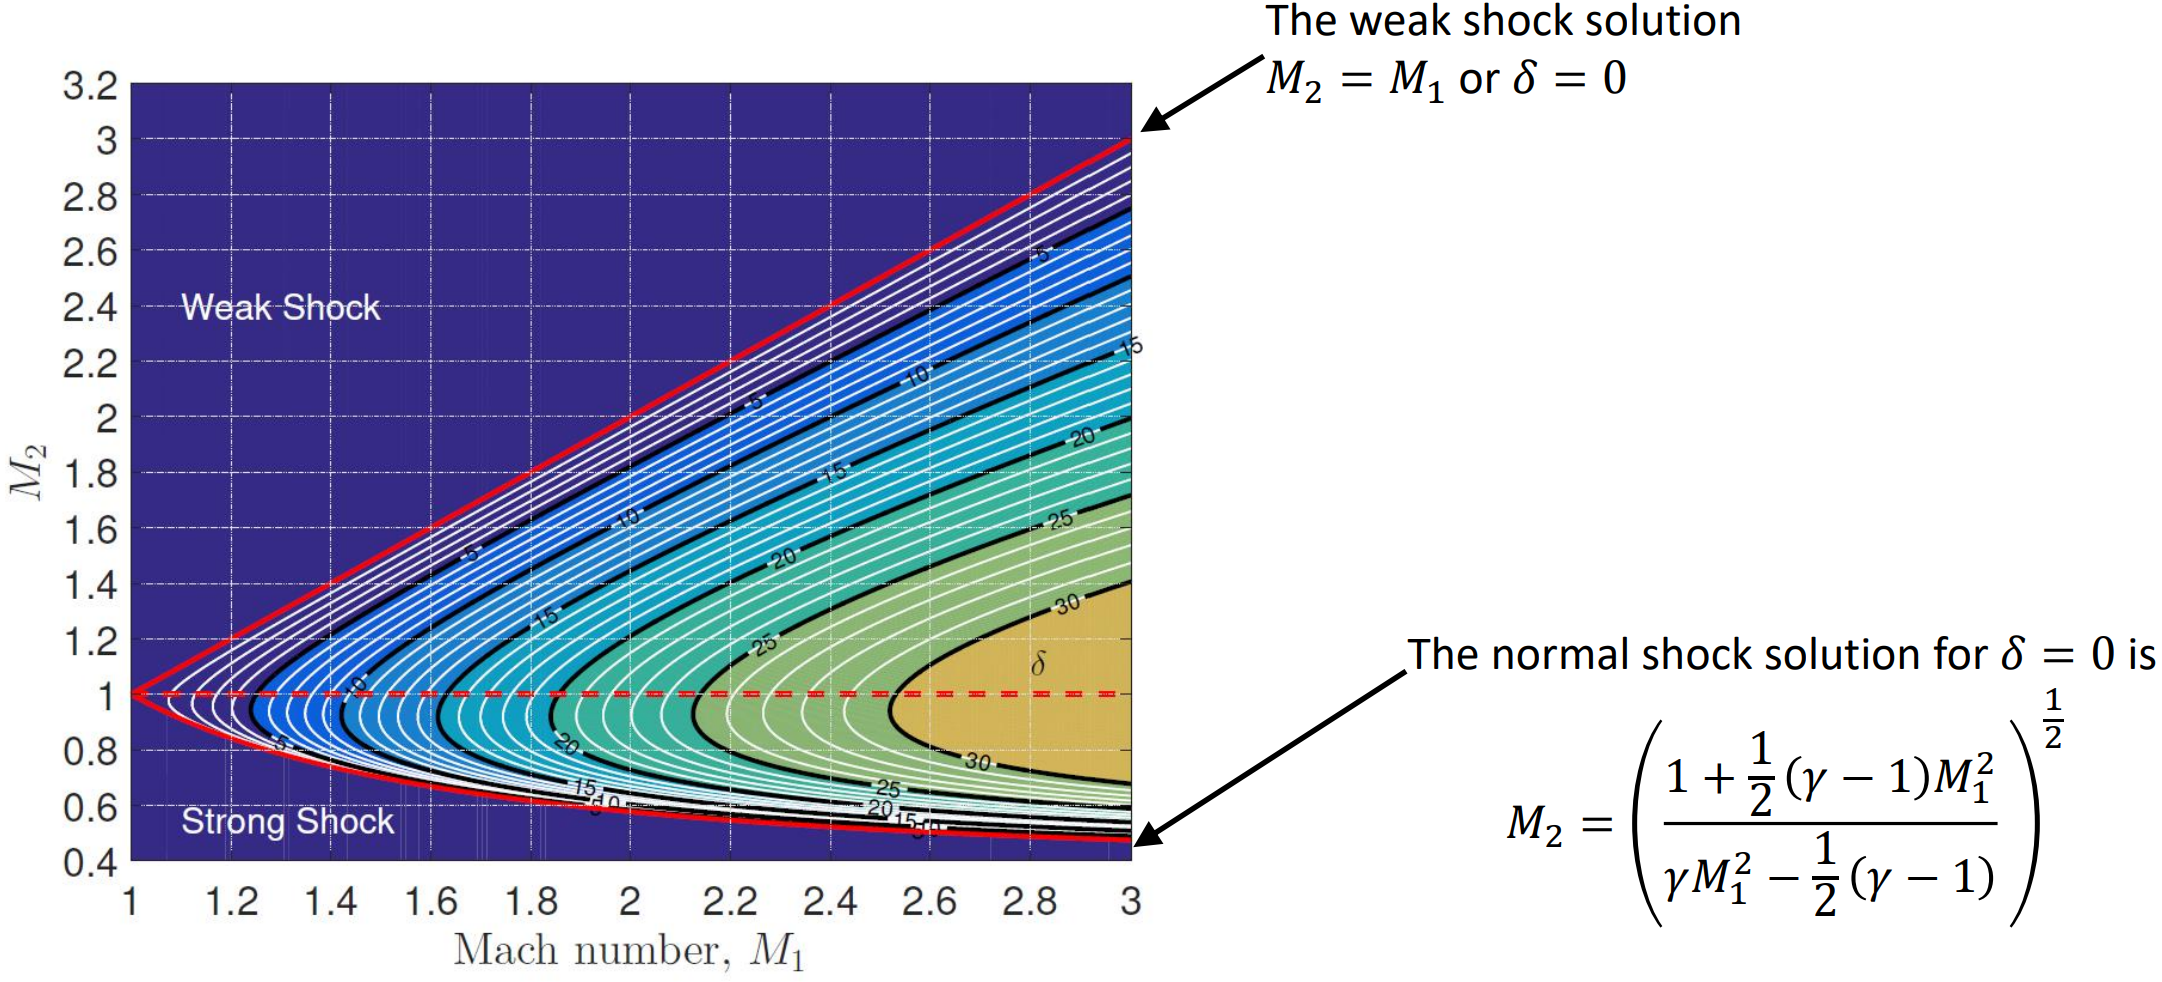
\includegraphics[width = 0.5\textwidth]{./img/diagram7.png}
\end{figure}
\begin{figure}[H]
  \centering
  \includegraphics[width = 0.5\textwidth]{./img/blockdiagram18.png}
\end{figure}
\chapter{First and Second Order Systems}
\section{First Order Systems}
All first order systems i.e. those with only $\frac{\dif x}{\dif t}$ take the following “standard” forms:
\begin{gather}
  \frac{X(s)}{Y(s)} = \frac{\alpha}{1+Ts} = \frac{\gamma}{1+\tau s}
\end{gather}
Where:
\begin{itemize}
  \item $\tau$, $\gamma$ is the \textbf{gain}
  \item T, $\tau$ is the \textbf{time constant}
\end{itemize}
This function is commonly known as an exponential time delay, or lag.
\subsection{Returning to the Time Domain}
To get the response of the system in the time domain we need to convert the transfer function from the Laplace domain. Tables of common inverse Laplace functions have already been created; all we need to do arrange our transfer function into one of these standard forms.
\begin{figure}[H]
  \centering
  \includegraphics[width = 1 \textwidth]{./img/laplacetransformationtable.png}
  \caption{Laplace Transformation Table}
\end{figure}
\subsubsection*{Example: Parallel Spring \& Damper (Laplace Domain found previously)}
\begin{gather}
  \frac{X(s)}{Y(s)} = \frac{\alpha}{1+Ts} = \frac{\gamma}{1+\tau s}
\end{gather}
Looking at the table, we can find the relevant inverse function; in this case (3rd from the top):
\begin{gather}
  a = \frac{1}{\tau}
\end{gather}
Hence:
\begin{gather}
  \frac{X(s)}{Y(s)} = \frac{\frac{\gamma}{\tau}}{\frac{1}{\tau}+s} = \frac{\gamma}{\tau}\frac{1}{\frac{1}{\tau}+s} \\
  x(t) = L^{-1}\left\{\frac{\gamma}{\tau}\frac{1}{\frac{1}{\tau}+s}\right\} \\
  = \frac{\gamma}{\tau}L^{-1}\left\{\frac{1}{\frac{1}{\tau}+s}\right\} \\
  = \frac{\gamma}{\tau}e^{-\frac{t}{\tau}}
\end{gather}
This is an exponential decay – the only variable needed to define the system is the time constant. The gain merely scales the response.
\begin{figure}[H]
  \centering
  \includegraphics[width = 0.9 \textwidth]{./img/graphs6.PNG}
\end{figure}
Having a negative time constant makes no physical sense, so the exception of $T=0$, the response will always be an exponential decay.
\subsection{Unit Step Response}
\begin{figure}[H]
  \centering
  \includegraphics[width = 0.65 \textwidth]{./img/graphs7.PNG}
\end{figure}
If a step input is given to a first order system, this will result in an exponential increase. This might be something like changing the room temperature. When talking about unit step input, the amplitude of the input will vary from 0 to 1. Some important definitions are:
\begin{itemize}
  \item Initial slope = $\frac{1}{time \ constant} = a$
  \item $T_r =$ Raising time = how quick the exponential function achieves 90\% of the final value
  \item $\tau$ = Time constant = how quick the exponential function achieves 63\% of the final value
  \item $T_s$ = Settling time = how quick the exponential function becomes constant
\end{itemize}
Remember, we have modelled mechanical and electrical systems, and arrived at the same equations. This could be biological, financial, meteorological… This is good, because you only need to understand one system to understand hundreds. However, this means the models can appear abstract (or possibly arbitrary), so it is important to keep in mind the physical systems we are trying to model.
\begin{figure}[H]
  \centering
  \includegraphics[width = 0.9 \textwidth]{./img/blockdiagram19.png}
  \caption{Left: Rate of decay determined by ratio of spring return force to viscous friction | Right: Rate of decay determined by total impedance of $R$ and $C$}
\end{figure}
\section{Second Order Systems}
The standard form for second order systems is shown below:
\begin{gather}
  G(s) = \gamma \frac{\omega_n^2}{s^2 + 2\zeta \omega_n s + \omega_n^2}
\end{gather}
Where:
\begin{itemize}
  \item $\gamma$ is the \textbf{gain}
  \item $\omega_n$ is the \textbf{natural frequency}
  \item $\zeta$ is the \textbf{damping ratio}
\end{itemize}
This function is known as a damped oscillator, in that it produces harmonic sinusoidal oscillations which decay over time. This type of system appears everywhere in physics, as well as in engineering. Even to the extent that some higher order systems are simplified to become second order, just because it is so well understood.
\subsubsection*{Example – Mass Spring Damper}
\begin{figure}[H]
  \centering
  \includegraphics[width = 0.3 \textwidth]{./img/massspringdamper.PNG}
\end{figure}
Consider a simple mechanical system Mass/Spring/Damper (MSD). As before, we wish to relate the input force to the output displacement i.e. Transfer function desired:
\begin{gather}
  G(s) = \frac{X(s)}{F(s)}
\end{gather}
Balancing forces as function of time:
\begin{gather}
  f(t) = f_S(t) + f_D(t) + f_I(t)
\end{gather}
Where:
\begin{itemize}
  \item $f_S(t) = kx(t)$
  \item $f_D(t) = c\frac{\dif x(t)}{\dif t}$
  \item $f_I(t) = m\frac{\dif^2 x(t)}{\dif t^2}$
\end{itemize}
So time domain force equilibrium is:
\begin{gather}
  f(t) = kx(t) + c\frac{\dif x(t)}{\dif t} + m\frac{\dif^2 x(t)}{\dif t^2}
\end{gather}
Converting to Laplace domain:
\begin{gather}
  F(s) = kX(s) + csX(s) + ms^2X(s) \\
  F(s) = X(s)(k + cs + ms^2) \\
  G(s) = \frac{X(s)}{F(s)} = \frac{1}{ms^2 + cs + k}
\end{gather}
To obtain the Laplace domain in the "standard" form, the coefficient of the highest order of $s$ on the denominator should be 1:
\begin{gather}
  G(s) = \frac{\frac{k}{m}}{s^2 + s\frac{c}{m} + \frac{k}{m}}\frac{1}{k} \\
  = \gamma \frac{\omega_n^2}{s^2 + 2\zeta \omega_n s + \omega_n^2}
\end{gather}
Where:
\begin{itemize}
  \item $\omega_n = \sqrt{\frac{k}{m}}$
  \item $\zeta = \frac{c}{2\sqrt{km}}$
  \item $\gamma = \frac{1}{k}$
\end{itemize}
\subsection{Returning to the Time Domain}
As before, we use the inverse Laplace transform to get the time domain response. To reiterate, the benefit of standard forms is that the transforms are given in the tables:
\begin{gather}
  G(s) = \gamma \frac{\omega_n^2}{s^2 + 2\zeta \omega_n s + \omega_n^2} \\
  x(t) = L^{-1} \left\{\frac{\omega_n^2}{s^2 + 2\zeta \omega_n s + \omega_n^2} \right\} \\
  \frac{x(t)}{x(0)} = \gamma \frac{\omega_n}{\sqrt{1-\zeta^2}}e^{-\zeta \omega_n t} sin(\omega_n \sqrt{1-\zeta^2}\cdot t)
\end{gather}
$\gamma$ is not shown as it is unaffected by the Laplace transform. The equation above looks complicated, but investigating each term yields:
\begin{gather}
  \gamma \frac{\omega_n}{\sqrt{1-\zeta^2}}
\end{gather}
$\gamma \ \omega_n \ \zeta$ are all constants, so the whole term is just a number.
\begin{gather}
  e^{-\zeta \omega_n t}
\end{gather}
It is an exponential function, which depending on whether $-\zeta \omega_n$ is positive or negative, increases or decays.
\begin{gather}
  sin(\omega_n \sqrt{1-\zeta^2}\cdot t)
\end{gather}
$\omega_n \ \zeta$ are just constants, so assuming $\zeta < 1$, this is just a sine wave.
\begin{figure}[H]
  \centering
  \includegraphics[width = 0.55 \textwidth]{./img/graphs8.PNG}
\end{figure}
This is an exponentially decaying sinusoidal oscillation, with:
\begin{itemize}
  \item Frequency: $\omega_n \sqrt{1-\zeta^2}\cdot t$
  \item Decay: $e^{-\zeta \omega_n t}$
  \item Gain: $\gamma \frac{\omega_n}{\sqrt{1-\zeta^2}}$
\end{itemize}
\subsection{Unit Step Response}
\begin{figure}[H]
  \centering
  \includegraphics[width = 0.65 \textwidth]{./img/graphs9.PNG}
\end{figure}
Some properties that should be known, but will be investigated later are:
\begin{itemize}
  \item Slope at the time step input is made $(t=0)$ = 0
  \item $T_p=$ Peak Time
  \item $T_s=$ Settling Time
  \item $T_r=$ Rise Time
  \item Overshoot
\end{itemize}
\section{Tutorial}
\subsection*{LRC Filter}
\begin{figure}[H]
  \centering
  \includegraphics[width = 0.25 \textwidth]{./img/lrcfilter.PNG}
\end{figure}
A more complex filtering circuit is an LRC filter, also known as a harmonic oscillator circuit, which allows for a narrower range of frequencies to be amplified or attenuated. These circuits are used in analogue radios with a variable capacitor or inductor connected to the dial to select the frequency. To describe the relationship between the input voltage $V_i$, and the voltage across the capacitor $V_C$:
\begin{gather}
  G(s) = \frac{V_C(s)}{V_i(s)}
\end{gather}
Balancing voltages using Kirchoff's Law:
\begin{gather}
  v_i = v_R + v_L + v_C
\end{gather}
Where:
\begin{itemize}
  \item $v_r(t) = i(t)R$
  \item $v_c(t) = \frac{1}{C}\int i(t)\dif t$
  \item $v_L(t) = L\frac{\dif i(t)}{\dif t}$
\end{itemize}
So time domain voltage is:
\begin{gather}
  v_i(t) = i(t)R + \frac{1}{C}\int i(t)\dif t + L\frac{\dif i(t)}{\dif t}
\end{gather}
Converting to Laplace domain:
\begin{gather}
  V_i(s) = I(s)R + \frac{1}{Cs}I(s) + LsI(s) \\
  V_i(s) = I(s) \left(R + \frac{1}{Cs} + Ls\right)
  \label{laplacedomain1}
\end{gather}
Getting the laplace domain and rearranging the $v_c(t)$ term yields:
\begin{gather}
  v_c(t) = \frac{1}{C}\int i(t)\dif t \\
  V_c(s) = \frac{1}{Cs}I(s) \\
  I(s) = V_C(s)Cs \label{Is}
\end{gather}
Inputting equation (\ref{Is}) into equation (\ref{laplacedomain1}):
\begin{gather}
  V_i(s) = CsV_c(s) \left(R + \frac{1}{Cs} + Ls\right) \\
  G(s) = \frac{V_C(s)}{V_i(s)} = \frac{1}{LCs^2 + CRs + 1}
\end{gather}
To obtain the Laplace domain in the "standard form":
\begin{gather}
  G(s) = \frac{\frac{1}{LC}}{s^2 + s\frac{R}{L} + \frac{1}{LC}} \\
  = \frac{\omega_n^2}{s^2 + 2\zeta \omega_n s + \omega_n^2}
\end{gather}
Where:
\begin{itemize}
  \item $\omega_n = \sqrt{\frac{1}{LC}}$
  \item $\zeta = \frac{R}{2}\sqrt{\frac{C}{L}}$
  \item $\gamma = 1$
\end{itemize}
\chapter{System Time Response - 1st order}
\section{Impulse functions/responses}
\subsection{Impulse response of a system: Dirac delta function}
A useful tool in analysing the transient response of a system is the impulse signal, a unit (amplitude = 1) pulse infinitesimally small, with area = 1. Formally this is known as the \textbf{Dirac delta function (impulse function)}.
\begin{figure}[H]
  \centering
  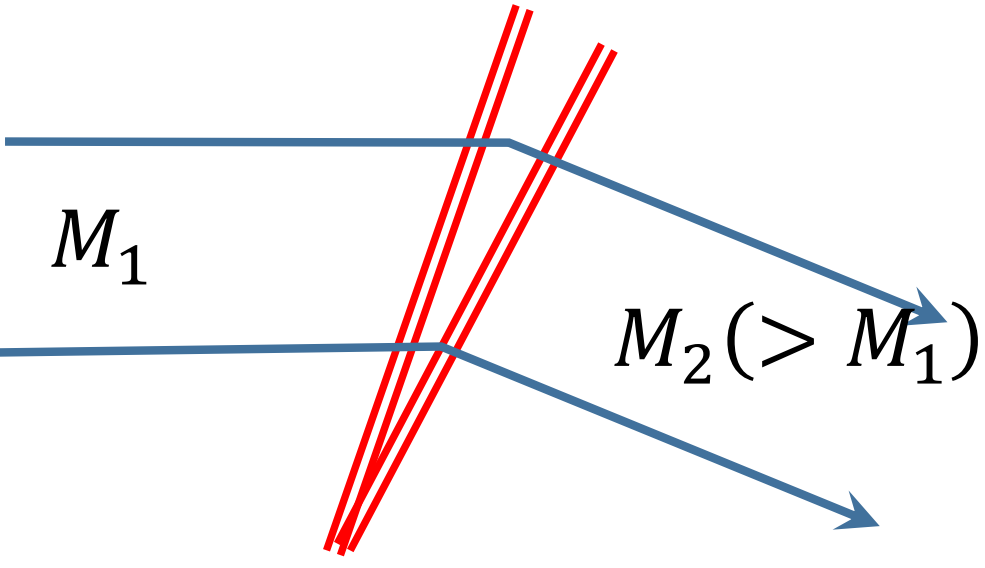
\includegraphics[width = 0.8\textwidth]{./img/diagram23.png}
\end{figure}
The Dirac delta function is a non-physical, singularity function with the follow definition:
\begin{equation}
  \delta (t) = \begin{cases}
    0 \textrm{ for } t \neq 0 \\
    \textrm{undefined for } t = 0
  \end{cases}
\end{equation}
but with the requirement that
\begin{equation}
  \int_{-\infty}^{\infty} \delta (t) \,\mathrm{d}t =1
\end{equation}
so taking the Laplace transform of this is also just 1
\begin{equation}
  \mathcal{L} (\delta (t)) = \int_{0^-}^{\infty} \delta (t) e^{-st} \,\mathrm{d}t = 1
\end{equation}
Thus, the impulse response of the system is equal to the transfer function and from this it can be shown that \textbf{any} arbitrary signal can be described as a summation of impulse responses.
\subsection{Impulse response on a first order system}
Take a first order response for example, the transfer function and thus the impulse response looks like this:
\begin{figure}[H]
  \centering
  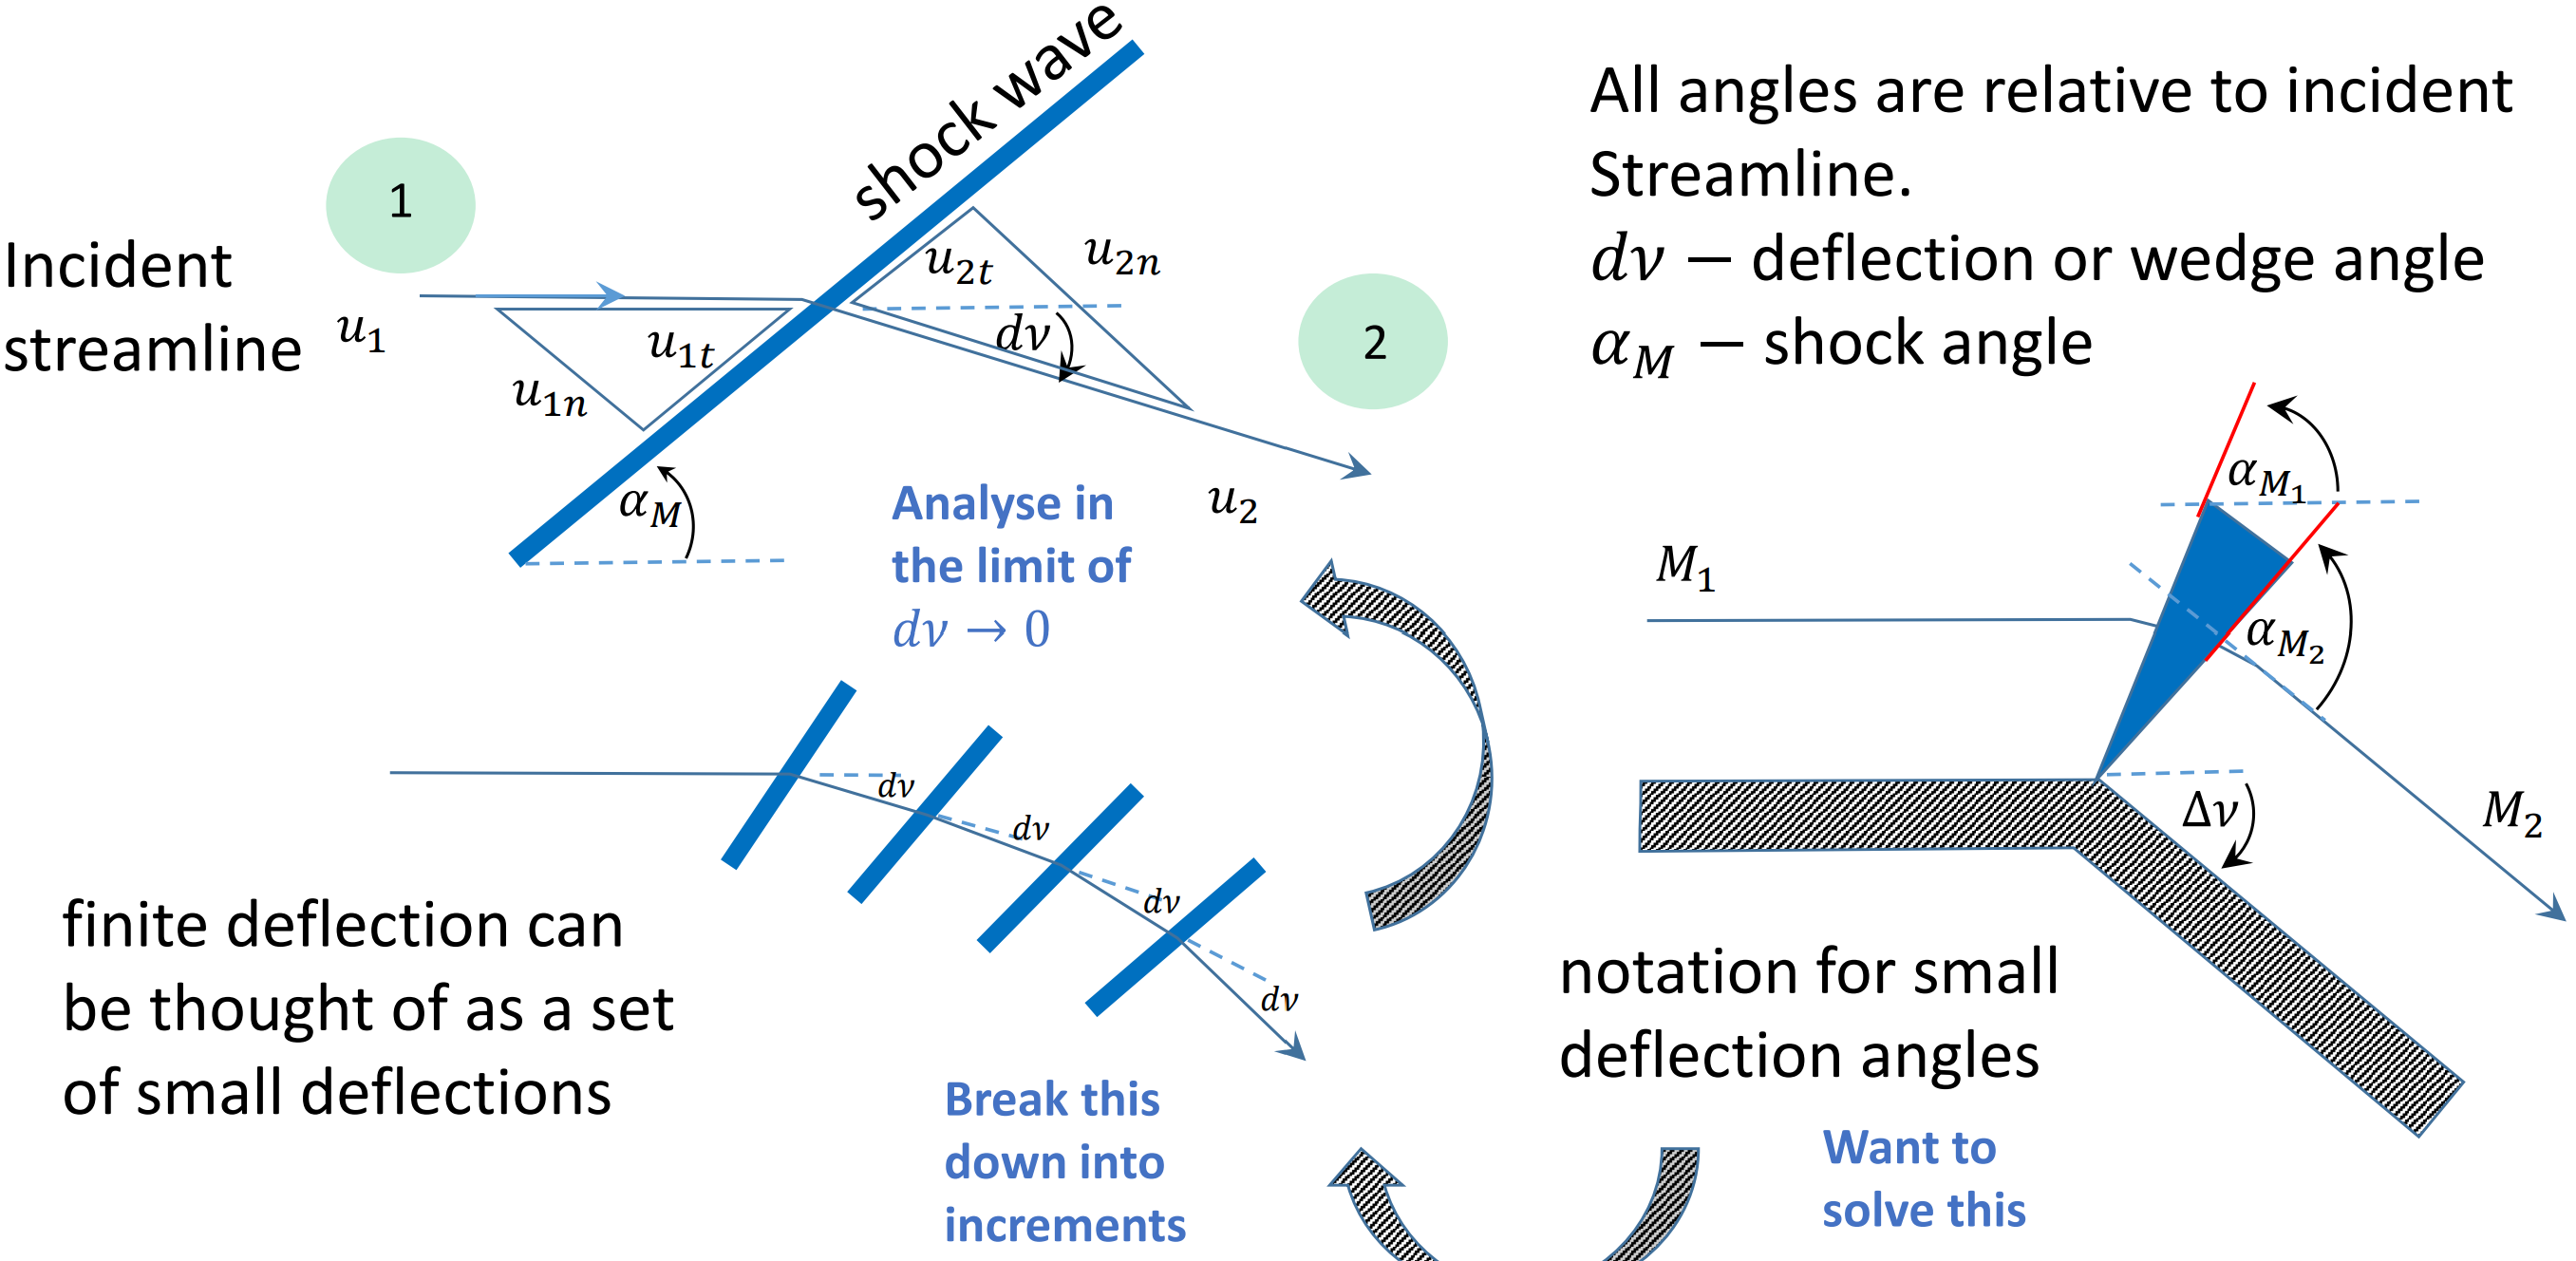
\includegraphics[width = 0.8\textwidth]{./img/diagram24.png}
\end{figure}
Due to our LTI assumptions:
\begin{itemize}
  \item Scaling the input scales the output
  \item Superposition of inputs equals superposition of outputs
  \item Time invariance
\end{itemize}
\subsection{Impulse response of a system}
\begin{figure}[H]
  \centering
  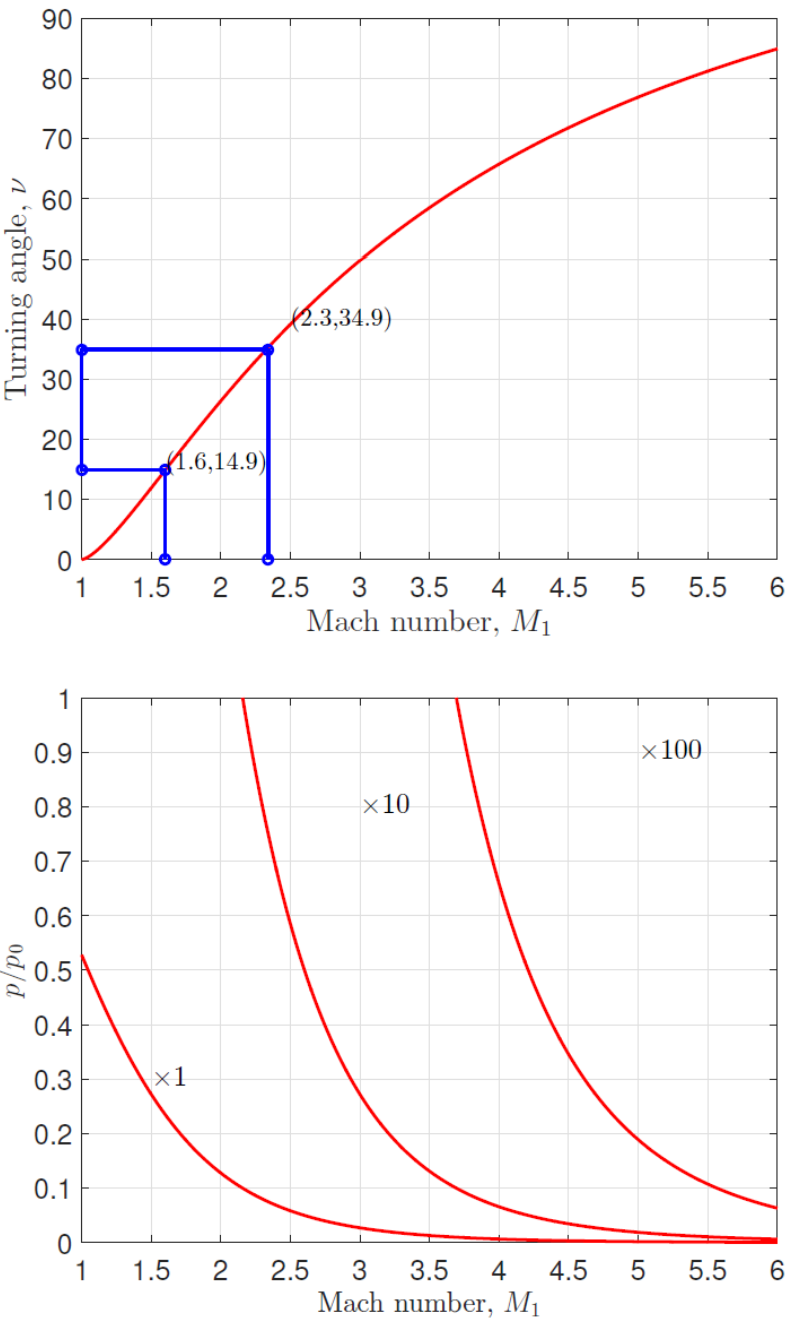
\includegraphics[width = 0.8\textwidth]{./img/diagram25.png}
\end{figure}
\subsubsection{Time vs Frequency Domain}
\begin{figure}[H]
  \centering
  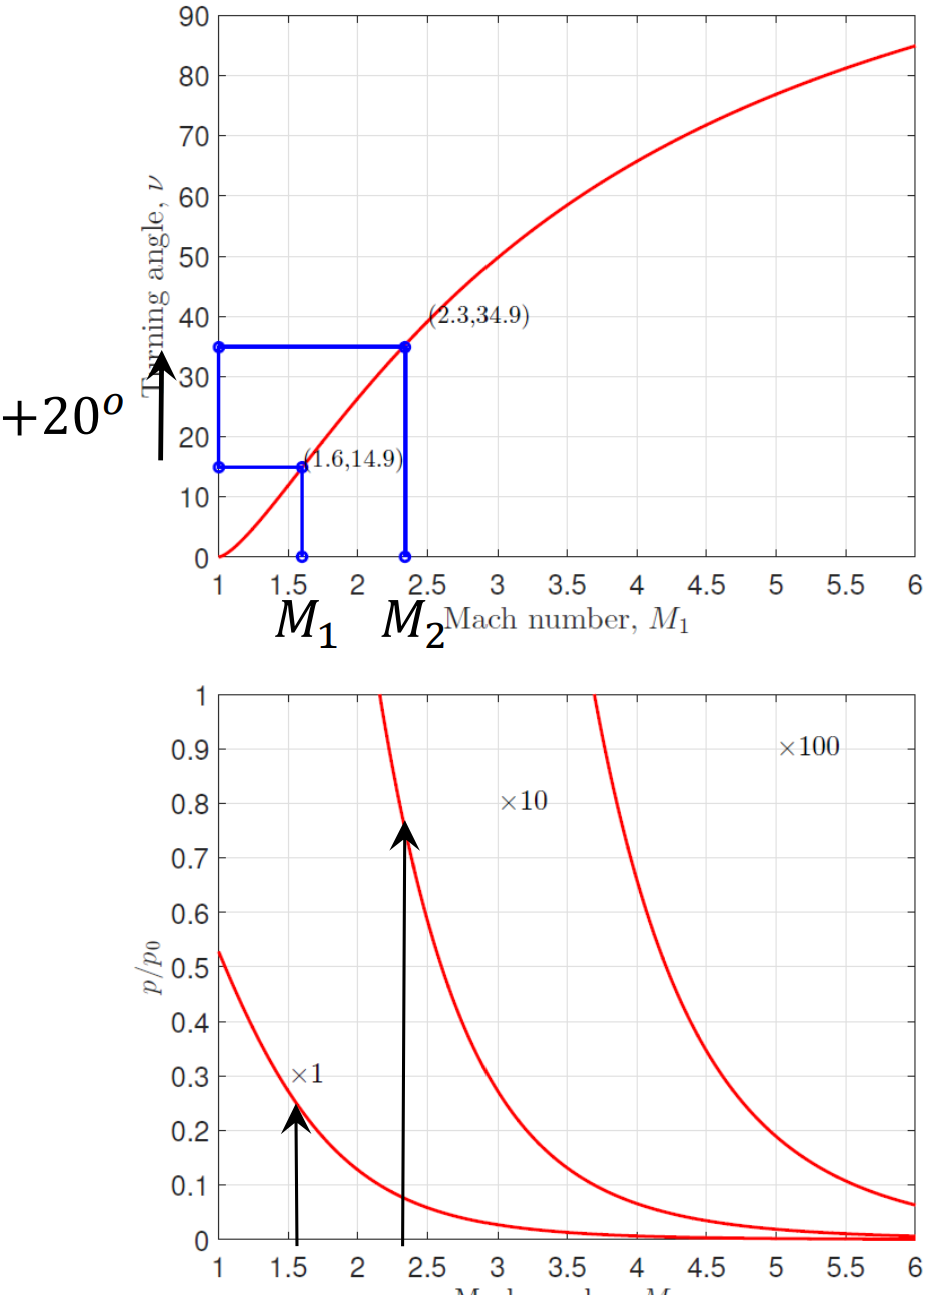
\includegraphics[width = 0.8\textwidth]{./img/diagram26.png}
\end{figure}
\begin{itemize}
  \item $u$ is the impulse function to the system
  \item $h$ is called the impulse response of the system
  \item $H$ is called the transfer function (TF) of the system
\end{itemize}
\begin{equation}
  y(t) = \int_{0}^{\infty} h(\tau) u (t-\tau) \,\mathrm{d}\tau = \int_{0}^{\infty} h(\tau - t)u(\tau) \,\mathrm{d}\tau
\end{equation}
with $0\leq \tau \leq t$
\begin{equation}
  y(t) = h(t) \cdot u(t)
\end{equation}
This is called convolution.
\begin{equation}
  Y(s) = H(s) \cdot U(s)
\end{equation}
This is called multiplication.
\subsubsection{Convolution example}
Essentially, the steps for convolving two signals are to first reflect the signal $g$, then offset the reflected signal. Then calculate the area under the graph for every offset, by sliding $-g$. The convolution at each time point is equal to the area under the intersection of functions. For two pulses, the result is a triangle wave:
\begin{figure}[H]
  \centering
  \includegraphics[width = 0.8\textwidth]{./img/diagram27.png}
\end{figure}
However, the calculations to obtain this result in the time domain are complicated, but are only multiplication in the Laplace domain.
\subsubsection{Getting the Time Response}
The procedure to describe the time response for LTI systems is thus:
\begin{itemize}
  \item Express the input, $u(t)$, in Laplace notation, $U(s)$
  \item Use this to find output $Y(s)$, usually by multiplying $U(s)$ by the transfer function $Y(s) = U(s)G(s)$
  \item Use inverse Laplace transforms (from tables) to express $Y(s)$ as a function of time, $y(t)$
\end{itemize}
\section{Input functions: Impulse - Step - Ramp}
Now we will consider some standard inputs and look at the response of first and second order systems:
\begin{itemize}
  \item Impulse
        \begin{itemize}
          \item The Laplace transform is 1, so the response to an impulse is by the definition the transfer function
        \end{itemize}
  \item Step
  \item Ramp
\end{itemize}
There are many others, particularly sinusoidal inputs or other discontinuous inputs, which are important in control loops, but we will focus on the two classic examples.
\subsection{Step input}
A step input is a discontinuous function, which is zero for all negative values of $t$ and 1 for all positive values.
\begin{figure}[H]
  \centering
  \includegraphics[width = 0.8\textwidth]{./img/diagram28.png}
\end{figure}
\subsubsection{Laplace transform}
\begin{gather}
  x(t) = U(t)\\
  \mathcal{L} \left\{ U(t) \right\} = \int_{0^-}^{\infty} e^{-st} \,\mathrm{d}t = \left[-\frac{1}{s} e^{-st}\right]_{0^-}^{\infty} \rightarrow \frac{1}{s}\\
\end{gather}
Or for a gain of A
\begin{gather}
  x(t) = AU(t) \\
  \mathcal{L} \left\{ AU(t) \right\} = \frac{A}{s}
\end{gather}
\subsubsection{Applications}
The step response is extremely useful in control theory for describing the behaviour of the system. In part because it incorporates the "transient" behaviour - from the sudden change from zero to one, as well as the "steady state" behaviour as the system settles down to a single value. IT also replicates many real world control applications such as:
\begin{itemize}
  \item Position control - move to a $X=10\si{\milli\meter}$ position and stay
  \item Speed control - go to 33 RPM
  \item Temperature - heat element on 3D printer to 230 \si{\celsius}
\end{itemize}
Also, unlike the Dirac impulse - it is physically realisable.
\subsection{Ramp input}
A ramp input has a value of $t$ for all $t$ values above zero and zero elsewhere, often is scaled by a gain A.
\begin{figure}[H]
  \centering
  \includegraphics[width = 0.8\textwidth]{./img/diagram29.png}
\end{figure}
\subsubsection{Laplace transform}
\begin{gather}
  x(t) = at\\
  \mathcal{L} \left\{ at \right\} \int_{0^-}^{\infty} ate^{-st} \,\mathrm{d}t = -a \left[ \frac{t}{s}e^{-st} \right]_{0}^{\infty} + a\int_{0}^{\infty} \frac{1}{s} e^{-st} \,\mathrm{d}t\\
  = a \left[ -\frac{1}{s^2}e^{-st} \right] \rightarrow \frac{a}{s^2}
\end{gather}
\subsubsection{Applications}
Ramp inputs are useful in understanding the steady state behaviour of a system i.e. when $t$ goes to infinity. Practical examples of control applications using ramp inputs are
\begin{itemize}
  \item Servo motors - shaft \textbf{position} rather than speed
  \item Ovens for PCB manufacturing etc. - strict linear \textbf{profile} of temperature required as opposed to "get to this temperature quickly"
  \item CNC milling machine, move in $X$ direction and constant rate
\end{itemize}
\subsection{Summary of Input Functions}
\begin{gather}
  \textrm{Impulse } F(s) = A\\
  \textrm{Step } F(s) = \frac{A}{s}\\
  \textrm{Ramp } F(s) = \frac{A}{s^2}
\end{gather}
For a \textbf{unit} response, $A=1$. We can apply these inputs to the LTI system by multiplying the transfer function by the input, both in terms of $s$.
\begin{figure}[H]
  \centering
  \includegraphics[width = 0.8\textwidth]{./img/diagram30.png}
\end{figure}
\section{First Order System Step Response}
Electromagnets are used in motors both rotary and linear, as well as in power transfer and also magnetic levitation in trains. First obtain the transfer function.
\begin{equation}
  \frac{I(s)}{V(s)}
\end{equation}
Balancing voltage gives:
\begin{equation}
  v(t) = v_R(t) + v_I(t)
\end{equation}
where
\begin{gather}
  v_R(t) = i (t) R\\
  v_I (t) = L\frac{\dif i(t)}{\dif t}
\end{gather}
Substitution gives:
\begin{equation}
  v(t) = Ri(t) + L\frac{\dif i(t)}{\dif t}
\end{equation}
In the Laplace domain
\begin{gather}
  V(s) = RI(s) + LsI(s)\\
  \frac{I(s)}{V(s)} = \frac{1}{(Ls + R)}
\end{gather}
For a \textbf{step} input of 1 \si{\volt} (unit step)
\begin{gather}
  V(s) = \frac{1}{s}\\
  I(s) = V(s) \frac{1}{(Ls + R)}\\
  =  \frac{1}{s(Ls + R)}
\end{gather}
Sadly there is no direct equivalent in the tables for this transform. The first takes is to split the expression up using partial fractions, into expressions that are give in the tables.
\begin{gather}
  I(s) = \frac{1}{s(Ls + R)} = \frac{\frac{1}{L}}{s(s+\frac{R}{L})} \textrm{ (remove coeff for s)}\\
  = \frac{k_1}{s} + \frac{k_2}{(s + \frac{R}{L})} \textrm{ partial fraction expansion}
\end{gather}
where
\begin{equation}
  k_1 (s + \frac{R}{L}) + k_2 s = \frac{1}{L}\\
\end{equation}
Looking at $s=0$
\begin{equation}
  k_1 \frac{R}{L} = \frac{1}{L} \rightarrow k_1 = \frac{1}{R}\\
\end{equation}
Looking at $s= -\frac{R}{L}$
\begin{equation}
  -k_2 \frac{R}{L} = \frac{1}{L} \rightarrow k_2 = -\frac{1}{R}
\end{equation}
Which yields
\begin{equation}
  I(s) = \frac{1}{R} \left[ \frac{1}{s} - \frac{1}{(s+\frac{R}{L})} \right]
\end{equation}
Looking at the Laplace tables, we can now use entries for $\frac{1}{s}$ and $\frac{1}{(s + a)}$, considering $t > 0 \therefore u(t) = 1$.
\begin{equation}
  I(t) = \frac{1}{R} \left[ 1 - e^{-\frac{R}{L}t}\right]
\end{equation}
Which has the familiar form of a first order exponential rise, with a steady state gain of $\frac{1}{R}$. Time constant $\tau = \frac{L}{R}$. For now assume that $L$ and $R = 1$, so gain and time constant are 1.
\begin{figure}[H]
  \centering
  \includegraphics[width = 0.8\textwidth]{./img/diagram31.png}
\end{figure}
Thus for a known time constant, it is possible to calculate the response at any point after the step. A common parameter of a first order system is the \textbf{settling time} which is the time taken to reach 95\% of the desired value, or $3\tau$. The inverse process is also used in system identification, because the response is so simple - we can measure the step response and calculate the time constant of the system. If we do convolution in the time domain you get the same too.
\begin{figure}[H]
  \centering
  \includegraphics[width = 0.8\textwidth]{./img/diagram32.png}
  \caption{Area under $f(\tau)g(1-\tau)$, blue line $f(\tau)$, red line $g(t-\tau)$, black line $(f+g)t$.}
\end{figure}
These "step responses" can be repeated for different values of $V$ and for different starting values of $I(t)$. The response will always be behind the input for all time constant $>0$, and thus these systems are referred to as \textbf{first order lags}.
\begin{figure}[H]
  \centering
  \includegraphics[width = 0.6\textwidth]{./img/diagram33.png}
\end{figure}
\section{First Order System Ramp Response}
For a \textbf{ramp} input of gain 1 (unit ramp)
\begin{gather}
  \frac{I(s)}{V(s)} = \frac{1}{(Ls+R)}\\
  V(s) = \frac{1}{s^2}\\
  I(s) = \frac{1}{s^2(Ls+R)} = \frac{\frac{1}{L}}{s^2(s+\frac{R}{L})}
\end{gather}
Again, this is not in the Laplace tables, so rearrange use partial fractions, giving us the general solution:
\begin{equation}
  I(t) = t - \tau \left(1 - e^{-\frac{t}{\tau}}\right)
\end{equation}
\begin{figure}[H]
  \centering
  \includegraphics[width = 0.6\textwidth]{./img/diagram34.png}
\end{figure}
After 4 time constants, we can say that the system is in the \textbf{steady state} where the difference between the input and output is no longer changing. The steady state lag is then equal to $\tau$
\section{Understanding Poles and Zeros}
As defined, the transfer function is a rational function in the complex variable $s = \sigma + jw$, that is
\begin{equation}
  G(s)=\frac{b_ms^m + b_{m-1}s^{m-1} + ... + b_1s + b_0}{a_ns^n + a_{n-1}s^{n-1}+...+a_1s + a_0}
\end{equation}
It is often convenient to factor the polynomials in the numerator and denominator, and to write the transfer function terms of those factors:
\begin{equation}
  G(s) = \frac{N(s)}{D(s)} = K \frac{(s-z_1)(s-z_2)...(s-z_{m-1})(s-z_m)}{(s-p_1)(s-p_2)...(s-p_{n-1})(s-p_n)}
\end{equation}
Where the numerator and denominator polynomials, $N(s)$ and $D(s)$, have real coefficients defined by the system's differential equation and $K = \frac{b_m}{a_n}$. Poles and zeros are found by
\begin{equation}
  N(s) = 0 \textrm{ and } D(s) = 0
\end{equation}
All of the coefficients of polynomials $N(s)$ and $D(s)$ are real, therefore  the poles and zeros must be either purely real, or appear in complex conjugate pairs.
\begin{quotation}
  The poles and zeros are properties of the transfer function and therefore of the differential equation describing the input-output system dynamics. Together with the gain constant, they completely characterize the differential equation, and provide a complete description of the system.
\end{quotation}
\subsection{Example}
A linear system is described by the differential equation:
\begin{gather}
  \frac{\dif^2y}{\dif t^2} + 2\frac{\dif y}{\dif t} + 5y = 3\frac{\dif u}{\dif t} + 12u\\
  \mathcal{L} \left\{ \frac{\dif^2y}{\dif t^2} + 2\frac{\dif y}{\dif t} + 5y \right\} = s^2 Y(s) + 2sY(s) + 5Y(s)\\
  \mathcal{L} \left\{ 3\frac{\dif u}{\dif t} + 12u \right\} = 3sU(s) + 12U(s)\\
  N(s) = 3s + 12 = 0 \rightarrow z_1 = -4\\
  D(s) = s^2 + 2s + 5 \rightarrow p_{1/2} = \frac{-2 \pm \sqrt{2^2 - 4\times 5}}{2} = -1 \pm j2\\
  G(s) = \frac{N(s)}{D(s)} = 3 \frac{(s-(-4))}{(s-(-1+j2))(s-(-1-j2))}
\end{gather}
\begin{figure}[H]
  \centering
  \includegraphics[width = 0.6\textwidth]{./img/diagram35.png}
\end{figure}
\subsection{s-Plane}
We can see how the time domain representation changes as we move around the s-plane. The imaginary axis corresponds to the sinusoidal component, and the real axis corresponds to the exponential.
\begin{figure}[H]
  \centering
  \includegraphics[width = 0.7\textwidth]{./img/diagram36.png}
\end{figure}
\section{Open Loop Motor Speed Control}
\begin{figure}[H]
  \centering
  \includegraphics[width = 0.7\textwidth]{./img/diagram37.png}
\end{figure}
For a DC motor connected to an inertial load, there is a combination of electrical and mechanical system equations determining the transfer function for angular position with respect to voltage.
\begin{equation}
  \frac{\Theta_m (s)}{v_a(s)}
\end{equation}
First consider the voltage balance:
\begin{equation}
  v_a = R_a i_a + L_a \frac{\dif i_a}{\dif t} + e_m
\end{equation}
Where $e_m$ is the back e.m.f of the motor. We can also write the above in Laplace:
\begin{equation}
  V_a(s) = R_a I_a (s) + L_a s I_a (s) + E_m (s)
\end{equation}
Next consider the torque balance in motor:
\begin{equation}
  T(t) = I_m \frac{\dif^2 \theta_m}{\dif t^2} + b \frac{\dif \theta_m}{\dif t}
\end{equation}
Which gives the following in Laplace:
\begin{equation}
  T(s) = I_m s^2 \Theta_m + bs\Theta_m (s)
\end{equation}
The electrical and mechanical sides are connected by motor constant which describe the characteristics of the motor (and given by manufacturer).
\begin{gather}
  e_m = K_e \frac{\dif \theta_m}{\dif t} \\
  T = K_t i_a
\end{gather}
Or in the Laplace domain:
\begin{gather}
  E_m (s) = K_e s \Theta_m (s)\\
  T(s) = K_t I_a (s)
\end{gather}
Combining this with our previous equations:
\begin{gather}
  V_a (s) = R_a I_a (s)+L_a s I_a (s) + E_m (s)\\
  T(s) = I_m s^2 \Theta_m (s) + bs\Theta_m (s)
\end{gather}
We arrive at the equation of voltage with respect to angular position:
\begin{equation}
  V_a (s) = \frac{R_a b}{K_t} \left[ s(\tau_a s +1)(\tau_m s +1)\right] \Theta_m (s) + K_e s\Theta_m (s)
\end{equation}
"Armature" time constant related to electrical side:
\begin{equation}
  \tau_a = \frac{L_a}{R_a}
\end{equation}
Motor time constant related to mechanical side:
\begin{equation}
  \tau_m = \frac{I_m}{b}
\end{equation}
The transfer function the becomes:
\begin{equation}
  \frac{\Theta_m(s)}{V_a(s)} = \frac{\frac{K_t}{R_a b}}{s\left[ \tau_m \tau_a s^2 + (\tau_m + \tau_a)s + \left( \frac{K_e K_t}{R_a b} + 1 \right)  \right]}
\end{equation}
Which looks very complicated, but we can make some simplifying assumptions, which quickly make things simple again. The electrical time constant is normally very small when compared to the mechanical one, as manufacturers try to keep the resistance and inductance low, so we can neglect $\tau_a$. The result, then simplifies to the following equation:
\begin{gather}
  \frac{\Theta_m(s)}{V_a(s)} = \frac{K}{s(\tau s + 1)}\\
  K = \frac{K_a K_t}{(bR_a + K_t K_b)}
\end{gather}
Where $K$ is the remaining leftover constants. This looks \textbf{much} simpler now, but we can take a step further, rather than consider the output position, lets look at the transfer function with respect to speed $\omega$
\begin{gather}
  \frac{\omega_m (s)}{V_a (s)} = \frac{\dif \left( \frac{\Theta_m (s)}{V_a (s)} \right)}{\dif t} = s \left( \frac{K}{s(\tau s +1)} \right)\\
  \frac{\omega_m (s)}{V_a (s)} = \frac{K}{(\tau s +1)}
\end{gather}
This is now just a first order system.
\chapter{System Time Response - 2nd order}
\section{Understanding poles and zeros}
As defined, the transfer function is a rational function in the complex variable $s = \sigma + j \omega$, that is:
\begin{align}
  G(s) = \frac{b_m s^m + b_{m-1}s^{m-1} + ... + b_1 s + b_0}{a_m s^m + a_{m-1}s^{m-1} + ... + a_1 s + a_0}
\end{align}
It is often convenient to factor the polynomials in the numerator and denominator, and to write the transfer function in terms of those factors:
\begin{align}
  G(s) = \frac{N(s)}{D(s)} = K\frac{(s-z_1)(s-z_2)...(s-z_{m-1})(s-z_m)}{(s-p_1)(s-p_2)...(s-p_{n-1})(s-p_n)}
\end{align}
where the numerator and denominator polynomials, $N(s)$ and $D(s)$, have real coefficients defined by the system's differential equation and $K = \frac{b_m}{a_n}$. Poles and zeros are found by
\begin{align}
  N(s) = 0 \textrm{ and } D(s) = 0
\end{align}
All of the coefficients of polynomials $N(s)$ and $D(s)$ are real, therefore the poles and zeros must be either purely real, or appear in complex conjugate pairs.
\begin{quote}
  The poles and zeros are properties of the transfer function, and therefore of the differential equation describing the input-output system dynamics. Together with the gain constant, the completely characterise the differential equation, and provide a complete description of the system.
\end{quote}
\subsection{Example}
A linear system is described by the differential equation:
\begin{align}
  \frac{\dif^2 y}{\dif t^2} + 2 \frac{\dif y}{\dif t} + 5y                              & = 3 \frac{\dif u}{\dif t} + 12 u                       \\
  \mathcal{L} \left\{ \frac{\dif^2 y}{\dif t^2} + 2 \frac{\dif y}{\dif t} + 5y \right\} & = s^2 Y(s) + 2s Y(s) + 5Y(s)                           \\
  \mathcal{L} \left\{ 3 \frac{\dif u}{\dif t} + 12 u \right\}                           & = 3sU(s) + 12U(s)                                      \\
  N(s) = 3s + 12 = 0 \rightarrow z_1                                                    & = -4                                                   \\
  D(s) = s^2 + 5s + 5 \rightarrow p_{\frac{1}{2}}                                       & = \frac{-2\pm\sqrt{2^2 - 4\times 5}}{2}  & = -1 \pm j2 \\
  G(s) = \frac{N(s)}{D(s)}                                                              & = 3\frac{s-(-4)}{(s-(-1+j2))(s-(-1-j2))}
\end{align}
\begin{figure}[H]
  \centering
  \includegraphics[width = 0.6\textwidth]{./img/diagram67.png}
\end{figure}
\subsection{s-Plane}
We can see how the time domain representation changes as we move around the s-plane. The imaginary axis corresponds to the sinusoidal component, and the real axis corresponds to the exponential.
\begin{figure}[H]
  \centering
  \includegraphics[width = 0.6\textwidth]{./img/diagram68.png}
\end{figure}
\section{Effect of damping ratio on the transfer function of a 2nd order system}
\subsection{2nd order transfer function}
The standard form of second order systems is shown below:
\begin{equation}
  G(s) = \gamma \frac{\omega_n^2}{s^2 + 2\zeta \omega_n s + \omega_n^2}
\end{equation}
where, $\gamma$ is gain, $\omega_n$ is the natural frequency and $\zeta$ is the damping ratio. Luckily the equation is 'standard form' and the time domain result is given directly in Laplace tables:
\begin{align}
  \gamma \frac{\omega_n}{\sqrt{1-\zeta^2}}e^{-\zeta \omega_n t} \sin{\left(\omega_n\sqrt{1-\zeta^2 t}\right)}
\end{align}
But this is only for $\zeta < 1$. Given the damping ratio for a mass spring damper
\begin{align}
  \zeta = \frac{c}{2\sqrt{mk}}, \ \omega_n = \sqrt{\frac{k}{m}}
\end{align}
It is clear the through the choice of $m$, $k$ and $c$ you could create a system with $\zeta \geq 1$.
\subsection{Characteristic equation}
\begin{align}
  G(s) = \gamma \frac{\omega_n^2}{s^2 + 2\zeta \omega_n s + \omega_n^2}
\end{align}
The denominator determines the behaviour of the transfer function, as the numerator is constant. This is known as the \textbf{characteristic equation}. It makes life much simpler if we first try to factor the denominator into first order terms like $(s+a)(s+b)$. So we require the roots of the equation:
\begin{align}
  s^2 + 2\zeta \omega_n s + \omega_n^2
\end{align}
Which can be determined from the quadratic equation:
\begin{align}
  s = -\zeta \omega_n \pm \omega_n \sqrt{\zeta^2 - 1}
\end{align}
Thus it is clear that the roots of the characteristic equations and thus the behaviour of the transfer function is determined by the damping ratio.
\begin{itemize}
  \item Overdamped: $\zeta > 1, \ s = -\zeta \omega_n \pm \omega_n \sqrt{\zeta^2 - 1}$
  \item Critically damped: $\zeta = 1, \ s = -\omega_n$
  \item Underdamped: $0 < \zeta < 1, \ s = -\zeta \omega_n \pm j \omega_n \sqrt{1-\zeta^2}$
  \item Undamped: $\zeta = 0, \ s = \pm j\omega_n$
\end{itemize}
Normally, only the underdamped case is given directly in the Laplace tables, so we need a bit of manipulation to get the others.
\subsection{Overdamped 2nd order system}
The characteristic equation has two real and negative roots
\begin{gather}
  \zeta > 1\\
  s = - \zeta \omega_n + \omega_n \sqrt{\zeta^2 - 1} = -\alpha\\
  s = - \zeta \omega_n - \omega_n \sqrt{\zeta^2 - 1} = -\beta\\
  \frac{\omega^2}{s^2 + 2\zeta\omega_n s+ \omega_n^2} = \frac{\alpha \beta}{(s+\alpha)(s+\beta)}
\end{gather}
Note: $\alpha \beta = \omega_n^2$. Using partial fractions we can split this into two separate first order systems:
\begin{align}
  \left(\frac{\alpha\beta}{\beta - \alpha}\right) \frac{1}{S + \alpha} + \left(\frac{\alpha\beta}{\alpha - \beta}\right)\frac{1}{S+\beta}
\end{align}
which gives the following in the time domain:
\begin{align}
  x(t) = \alpha \beta \left(\frac{e^{-\alpha t}}{\beta - \alpha} + \frac{e^{-\beta t}}{\alpha - \beta}\right)
\end{align}
\begin{figure}[H]
  \centering
  \includegraphics[width = 0.6\textwidth]{./img/diagram69.png}
\end{figure}
There is no sinusoidal term anymore, the response is only a combination of exponential decays, a more complex but similar response to a first order system.
\subsection{Critically damped 2nd order system}
Special case with a single repeated root:
\begin{gather}
  \zeta = 1\\
  s = -\omega_n\\
  \frac{\omega^2}{s^2 + 2\zeta\omega_n s+ \omega_n^2} = \frac{\omega_n^2}{(s+\omega_n)^2}
\end{gather}
To get the time response, we first take the numerator outside:
\begin{gather}
  L^{-1}\left[ \frac{\omega_n^2}{(s+\omega_n)^2} \right] = \omega_n^2 L^{-1} \left[ \frac{1}{(s+\omega_n)^2} \right]
\end{gather}
We can then use the inverse Laplace rule:
\begin{gather}
  \textrm{if } L^{-1} \left[F(S)\right] = f(t) \textrm{ then } L^{-1} \left[F(s-a)\right] = e^{at} f(t)\\[10pt]
  \omega_n^2 L^{-1} \left[\frac{1}{(s+\omega_n^2)}\right] = \omega_n^2 e^{-\omega_n t} L^{-1} \left[\frac{1}{s^2}\right]
\end{gather}
$\frac{1}{s^2}$ is the standard form of a ramp, or more generally from the Laplace tables:
\begin{align}
  L^{-1}\left[\frac{n!}{s^{n+1}}\right] = t^n
\end{align}
\begin{figure}[H]
  \centering
  \includegraphics[width = 0.6\textwidth]{./img/diagram70.png}
\end{figure}
The result is an exponential decay, multiplied by a ramp $= \omega_n^2 e^{-\omega_n t} t$.
\subsection{Undamped 2nd order system}
Another special case with two imaginary roots:
\begin{gather}
  \zeta = 0\\
  s = \pm j \omega_n\\
  \frac{\omega^2}{s^2 + 2\zeta\omega_n s+ \omega_n^2} = \frac{\omega_n^2}{s^2 + \omega_n^2}
\end{gather}
Which, using the standard form for an oscillator is:
\begin{equation}
  \omega_n L^{-1} \left[ \frac{\omega_n}{s^2 + \omega_n^2} \right] = \omega_n \sin{(\omega_n t)}
\end{equation}
\begin{figure}[H]
  \centering
  \includegraphics[width = 0.6\textwidth]{./img/diagram71.png}
\end{figure}
So the response is now just a sinusoid, with no exponential components.
\section{Applying a step input to 2nd order systems - damping}
Previously we saw for a step of $A$ the output can be calculated from
\begin{gather}
  Y(s) = \frac{A}{s} G(s)\\
  Y(s) = \frac{1}{s} \cdot \frac{\omega_n^2}{s^2 + 2\zeta \omega_n s \omega_n^2}
\end{gather}
All of the following can be found through partial fraction decomposition and the standard Laplace tables.
\subsection{Overdamped step input response of 2nd order systems}
\begin{gather}
  \zeta > 1\\
  y(t) = \left(1 = \frac{\beta e^{-\alpha t}}{\alpha - \beta} - \frac{\alpha e^{-\beta t}}{\alpha - \beta}\right)
\end{gather}
\begin{figure}[H]
  \centering
  \includegraphics[width = 0.8\textwidth]{./img/diagram72.png}
\end{figure}
The slowest rise from the $\beta$ exponential dominates, as $\zeta$ increases the $\alpha$ term becomes negligible, and system becomes first order.
\subsection{Critically damped step input response of 2nd order systems}
\begin{gather}
  \zeta = 1\\
  y(t) = \left(1 - e^{-\omega_n t} - \omega_n e ^{-\omega_n t} t\right)
\end{gather}
\begin{figure}[H]
  \centering
  \includegraphics[width = 0.6\textwidth]{./img/diagram73.png}
\end{figure}
Fastest possible rise without oscillating.
\subsection{Underdamped step input response of 2nd order systems}
\begin{gather}
  0 < \zeta < 1 \\
  y(t) = 1 - \frac{1}{\sqrt{1 - \zeta^2}}e^{-\zeta \omega_n t} \sin{\left(\omega_n \sqrt{1-\zeta^2 t} + \arccos{\zeta}\right)}
\end{gather}
\begin{figure}[H]
  \centering
  \includegraphics[width = 0.6\textwidth]{./img/diagram74.png}
\end{figure}
It is sometimes written in terms of the damped natural frequency:
\begin{gather}
  \omega_d = \omega_n \sqrt{1-\zeta^2}\\
  y(t) = 1 - \frac{1}{\sqrt{1-\zeta^2}} e^{-\zeta \omega_n t} \sin{\left(\omega_d t + \arccos{\zeta}\right)}
\end{gather}
\subsection{Undamped step input response of 2nd order systems}
\begin{align}
  \zeta = 0 \\
  y(t) = \left(1 - \cos{(\omega_n t)}\right)
\end{align}
As damping ratio reaches zero, the oscillations no longer decay
\begin{equation}
  \omega_d = \omega_n \sqrt{1 - 0} = \omega_n
\end{equation}
So oscillations are at natural frequency with pi phase shift.
\begin{figure}[H]
  \centering
  \includegraphics[width = 0.6\textwidth]{./img/diagram75.png}
\end{figure}
\section{Underdamped step input responses}
\subsection{Performance Criteria}
Rise time $t_r$ is the time to reach steady state value (for first time). Peak time $t_p$ is the time to initial overshoot.
\begin{figure}[H]
  \centering
  \includegraphics[width = 0.6\textwidth]{./img/diagram76.png}
\end{figure}
Peak overshoot - value of overshoot above steady state: $ y(t_p) - y_{ss} = A$. Settling time $t_s$. Time for response to reach and maintain a certain ratio of the steady state value. Commonly $\pm 5\%$ or $\pm 2\%$
\begin{figure}[H]
  \centering
  \includegraphics[width = 0.6\textwidth]{./img/diagram77.png}
\end{figure}
These criteria can be read from the graph, but having equations for them allows for a system parameters $\zeta$ and $\omega_n$ to be estimated. It is also useful for quantifying the effect of $\zeta$ on the response. Rise time can be found by setting the response $y$ to 1 and then rearranging:
\begin{equation}
  t_r = \frac{1}{\omega_d} \left( \pi - \arctan{\left( \frac{\sqrt{1-\zeta^2}}{\zeta} \right)} \right)\\
  \omega_d = \omega_n \sqrt{1-\zeta^2}
\end{equation}
So a higher damping ratio gives a slower response, but lower damping ratios give a more oscillatory response. Also, that for \textbf{overdamped} systems where $\zeta > 1$, the rise time is infinite. The peak time occurs at half a period of oscillation, or can be found from finding first minima by setting derivative to zero:
\begin{equation}
  t_p = \frac{\pi}{\omega_n\sqrt{1 - \zeta^2}} = \frac{\pi}{\omega_d}
\end{equation}
\subsubsection{Peak overshoot}
\begin{gather}
  1 + A = 1 - \frac{1}{\sqrt{1 - \zeta^2}} e^{\frac{-\zeta \pi}{\sqrt{1-\zeta^2}}}\sin{\left(\pi + \arccos{\zeta}\right)}\\[10pt]
  A = \frac{\sqrt{1-\zeta^2}}{\sqrt{1-\zeta^2}} e^{\frac{-\zeta \pi}{\sqrt{1-\zeta^2}}} = e^{\frac{-\zeta \pi}{\sqrt{1-\zeta^2}}}
\end{gather}
Often, this is given as a percentage:
\begin{equation}
  A = 100 e^{\frac{-\zeta \pi}{\sqrt{1-\zeta^2}}}
\end{equation}
This can be rearranged to find the required damping ratio for a required overshoot:
\begin{gather}
  \zeta = \sqrt{\frac{\left(\ln{\frac{A}{100}}\right)^2}{\pi^2 + \left(\ln{\frac{A}{100}}\right)^2}}\\
  \frac{A}{100} \rightarrow 0\\
  \zeta \rightarrow 1
\end{gather}
\subsubsection{Settling time}
The envelope of the oscillation is described by the decaying exponential term, so to find the settling time, we can just consider this term alone.
\begin{figure}[H]
  \centering
  \includegraphics[width = 0.6\textwidth]{./img/diagram78.png}
\end{figure}
For example, the common target is 5\%:
\begin{gather}
  e^{-\zeta \omega_n t_s} = 0.05\\
  -\zeta \omega_n t_s = \ln{0.05} = -3\\
  t_s (5\%) = \frac{3}{\zeta \omega_n}
\end{gather}
Or similarly:
\begin{equation}
  t_s (2\%) = \frac{4}{\zeta \omega_n}
\end{equation}
So settling time increases with a \textbf{decreasing} damping ratio, for underdamped systems only.
\section{Ramp input function responses}
\subsection{Applying inputs}
Previously, we saw for a step of $A$ the output can be calculated from:
\begin{gather}
  Y(s) = \frac{A}{s^2} G(s)\\
  Y(s) = \frac{1}{s^2} \frac{\omega_n^2}{s^2 + 2\zeta \omega_n s + \omega_n^2}
\end{gather}
All the following can be found through partial fraction decomposition and the standard Laplace tables (and loads more manipulation!). All these expressions are pretty complicated, but the important thing is to understand how the response changes with damping ratio, which follows a similar trend to the step response.
\subsection{Undamped response}
$\zeta = 0$: undamped - sustained oscillations around ramp input $y = t$.
\begin{equation}
  y(t) = \left(t - \frac{\sin(\omega_n t)}{\omega_n}\right)
\end{equation}
\begin{figure}[H]
  \centering
  \includegraphics[width = 0.6\textwidth]{./img/diagram79.png}
\end{figure}
\subsection{Underdamped response}
$\zeta < 1$: underdamped - exponential decaying oscillatory response around delayed ramp function.
\begin{multline}
  y(t) = \frac{1}{\omega_n} \left( \omega_n t - 2\zeta + e^{-\zeta \omega_n t} \left( 2\zeta \cos\left( \omega_n t\sqrt{1 - \zeta^2} \right) \right. \right. \\
  \left. \left. - \frac{1}{\sqrt{1-\zeta^2}} \left( 1 - 2\zeta^2 \right) \sin \left( \omega_n t\sqrt{1-\zeta^2} \right) \right) \right)
\end{multline}
\begin{figure}[H]
  \centering
  \includegraphics[width = 0.6\textwidth]{./img/diagram80.png}
\end{figure}
\subsection{Critically damped response}
$\zeta = 1$: Critically damped - fastest response with no overshoot, still lagging input.
\begin{equation}
  y(t) = \frac{1}{\omega_n} \left(\omega_n t - 2 + \left(2 + \omega_n t\right)e^{-\omega_n t}\right)
\end{equation}
\begin{figure}[H]
  \centering
  \includegraphics[width = 0.6\textwidth]{./img/diagram81.png}
\end{figure}
\subsection{Overdamped response}
$\zeta > 1$: overdamped - cannot overshoot, lag increases.
\begin{equation}
  y(t) = \left(t -\frac{2\zeta}{\omega_n} + \frac{\beta e^{-\alpha t}}{\alpha - \beta} - \frac{\alpha e^{-\beta t}}{\alpha - \beta} \right)
\end{equation}
\begin{figure}[H]
  \centering
  \includegraphics[width = 0.6\textwidth]{./img/diagram82.png}
\end{figure}
\subsection{Summary}
Much more complicated response! but follows the same pattern as with the step response with changing damping ratio. The most important thing to notice here, is that the system does not match desired value - there is still a lag:
\begin{equation}
  y(t) = t - \frac{2\zeta}{\omega_n}
\end{equation}
So a low damping ratio is needed to closely match the input value, but this comes at the expense of overshoot and settling time.
\section{Transfer function - unity feedback system}
Recall the block diagram for a closed loop feedback system, in this case with 'unity' feedback - i.e. the error signal is passed directly to the summation junction:
\begin{figure}[H]
  \centering
  \includegraphics[width = 0.9\textwidth]{./img/diagram83.png}
\end{figure}
$G(s)$ is referred to as the \textbf{forward loop transfer function}, i.e. the combined transfer function of all the amplifiers controller, plant, systems in the feedforward path. In the case of unity feedback, it is also the \textbf{open loop transfer function}. We can find the overall transfer function $F(s)$ or \textbf{closed loop transfer function} through a bit of manipulation:
\begin{gather}
  \theta = \theta_i - \theta_0\\
  G(s)\theta = \theta_0\\
  \theta_0 = G(s) (\theta_i - \theta_0)\\
  \frac{\theta_0}{\theta_i} = F(s) = \frac{G(s)}{1 + G(s)}
\end{gather}
Or more generally for a non unity gain system:
\begin{figure}[H]
  \centering
  \includegraphics[width = 0.6\textwidth]{./img/diagram84.png}
\end{figure}
\begin{equation}
  F_1 = \frac{\theta_0}{\theta_i} = \frac{G_1}{1 + G_1 H}
\end{equation}
Lets take an example to show how this transfer function can relate to the systems we have studied so far.
\section{Summary}
\begin{figure}[H]
  \centering
  \includegraphics[width = 0.6\textwidth]{./img/diagram85.png}
\end{figure}
The overdamped ($\zeta > 1$) and critically damped ($\zeta = 1$) responses are seldom desirable for control systems due to their long settling time. $\zeta = 0.7$ gives a fast response without excessive overshoot or oscillations.
\begin{figure}[H]
  \centering
  \includegraphics[width = 0.6\textwidth]{./img/diagram86.png}
\end{figure}
The response of second order systems is much more complicated than that of a first order system, with considerably different responses arising from changes in damping ratio.
\begin{figure}[H]
  \centering
  \includegraphics[width = 0.6\textwidth]{./img/diagram84.png}
\end{figure}
Negative feedback systems have a transfer function of the form:
\begin{equation}
  F_1 = \frac{\theta_0}{\theta_i} = \frac{G_1}{1 + G_1 H}
\end{equation}
Which for a remote position servo is equal to:
\begin{equation}
  F(s) = \frac{\Theta_0 (s)}{\Theta_i (s)} = \frac{\frac{k}{I}}{s^2 + \frac{f}{I}s + \frac{k}{I}}
\end{equation}
Where $\omega_n = \sqrt{\frac{k}{I}}$ and $\zeta = \frac{f}{2\sqrt{kI}}$. The gain determines the damping ratio, and this the characteristics of the response of the system.
\chapter{The s-plane and Steady State Errors}
\section{The s-Plane - Poles and Zeroes}
\subsection{Example: Servo as a second order system}
\begin{figure}[H]
  \centering
  \includegraphics[width = 0.6\textwidth]{./img/diagram87.png}
  \caption{}
\end{figure}
We saw last week that a DC motor servo with position control has a transfer function of a second order system.
\begin{figure}[H]
  \centering
  \includegraphics[width = 0.6\textwidth]{./img/diagram88.png}
  \caption{}
\end{figure}
\begin{align}
  F(s) = \frac{G(s)}{1+G(s)} = \frac{\frac{K}{I}}{s^2 + \frac{f}{I}s + \frac{K}{I}}
\end{align}
Where, $\omega_n = \sqrt{\frac{k}{I}}$ (with increasing $k$, $\omega_n$ increases) and $\zeta = \frac{f}{2\sqrt{kI}}$ (with increasing $k$, $\zeta$ decreases).
\begin{figure}[H]
  \centering
  \includegraphics[width = 0.6\textwidth]{./img/diagram89.png}
  \caption{}
\end{figure}
The overdamped ($\zeta > 1$) and critically damped ($\zeta = 1$) responses are seldom desirable for control systems due to their long settling time. $\zeta = 0.7$ gives a fast response without excessive overshoot or oscillations.
\subsection{Transfer functions}
As we have seen, transfer functions allow for important characteristics of the system response to be determined, without having to solve complete differential equations. Generally, transfer functions can be derived from the differential equations thusly:
\begin{multline}
  a_n \frac{\dif^n y}{\dif t^n} + a_{n-1}\frac{\dif^{n-1} y}{\dif t^{n-1}} + ... + a_2 \frac{\dif^2 y}{\dif t^2} + a_1 \frac{\dif y}{\dif t} + a_0 y =\\ b_0 x + b_1 \frac{\dif x}{\dif t} + b_2 \frac{\dif^2 x}{\dif t^2} + ... + b_{m-1}\frac{\dif^{m-1} x}{\dif t^{m-1}} + b_m \frac{\dif^{m} x}{\dif t^m} \label{TFEq1}
\end{multline}
(Solving equation (\ref{TFEq1}) is hard!). Where $a$ are the output coefficients and $b$ are the input coefficients, combined these \textbf{entirely} characterise the system. The Laplace domain transfer function is then given by:
\begin{align}
  G(s) = \frac{b_m s^m + b_{m-1} s^{m-1} + ... + b_1 s + b_0}{a_n s^n + a_{n-1} s^{n-1} + ... + a_1 s + a_0}
\end{align}
\subsection{System poles and zeroes}
As defined, the transfer function is a rational function in the complex variable $s=\sigma + j\omega$, that is:
\begin{equation}
  G(s) = \frac{b_m s^m + b_{m-1} s^{m-1} + ... + b_1 s + b_0}{a_n s^n + a_{n-1} s^{n-1} + ... + a_1 s + a_0}
\end{equation}
It is often convenient to factor the polynomials in the numerator and denominator; and to write the transfer function in terms of those factors:
\begin{equation}
  G(s) = \frac{N(s)}{D(s)} = K\frac{(s-z_1)(s-z_2)...(s-z_{m-1})(s-z_m)}{(s-p_1)(s-p_2)...(s-p_{n-1})(s-p_n)}
\end{equation}
where the numerator and denominator polynomials, $N(s)$ and $D(s)$, have real coefficients defined by the system's differential equation. Poles and zeroes are found by:
\begin{equation}
  N(s) = 0 \textrm{ and } D(s) = 0
\end{equation}
All of the coefficients of polynomials $N(s)$ and $D(s)$ are real, therefore the poles and zeroes must be either purely real, or appear in complex conjugate pairs.
\begin{quotation}
  The poles and zeros are properties of the transfer function, and therefore of the differential equation describing the input-output system dynamics. Together with the gain constant, they completely characterise the differential equation and provide a complete description of the system.
\end{quotation}
\subsection{Transfer functions in the s-plane}
A system is characterised by its poles and zeroes as they allow the reconstruction of the input/output differential equation. It is possible to get a sense of the system dynamics from plotting the poles and zeroes graphically on the s-plane. A pole is commonly represented by a cross ($\times$) and a zero by a circle ($\circ$). Recall that, as $s$ is a complex number, we can plot the value on a plane, with a real and imaginary axis.
\begin{equation}
  s = \sigma + j\omega
\end{equation}
By plotting the locations of the poles and zeroes on this plane, we can obtain a considerable amount of information about the response of the system without having to take the inverse Laplace transform. Each pole corresponds to a component of the time domain response, so from the plot it is possible to determine:
\begin{itemize}
  \item What components exist
  \item Their relative important (and possible simplifications)
  \item How they change with gain
\end{itemize}
\subsubsection{Real poles - exponentials}
First lets look at the real component only:
\begin{gather}
  s = \sigma\\
  e^s \rightarrow e^{-\sigma}
\end{gather}
Corresponding to $Ce^{-\sigma t}$
\begin{figure}[H]
  \centering
  \includegraphics[width = 0.6\textwidth]{./img/diagram90.png}
  \caption{}
\end{figure}
Poles located on the real axis have an exponential component only, with the pole location determining the rate of decay. Poles close to origin decay slowly, where poles far away decay rapidly. Poles located in the right hand side exponentially \textbf{increase}, whereas poles on the left hand side \textbf{decrease}. A pole on the origin is a flat 'DC' response.
\subsubsection{Imaginary poles - sinusoids}
First lets looks at the imaginary component only:
\begin{gather}
  s = \pm j\omega\\
  e^s \rightarrow e^{\pm j\omega}
\end{gather}
Which, from Euler's formula gives a sinusoidal response:
\begin{equation}
  e^{jx} = \cos{x} + j\sin{x}
\end{equation}
Poles located on the imaginary axis are in conjugate pairs.
\begin{figure}[H]
  \centering
  \includegraphics[width = 0.6\textwidth]{./img/diagram91.png}
  \caption{}
\end{figure}
The imaginary poles generate an oscillatory component with a constant amplitude. Poles closer to the origin have a low frequency, which increases the further poles are from the origin.
\subsubsection{Complex poles}
Commonly, the poles are a combination of the two components.
\begin{figure}[H]
  \centering
  \includegraphics[width = 0.6\textwidth]{./img/diagram92.png}
  \caption{}
\end{figure}
A complex conjugate pair of complex poles generates an exponentially decaying sinusoid in the form:
\begin{equation}
  Ae^{-\sigma t}\sin{\left(\omega t + \phi\right)}
\end{equation}
$A$ and $\phi$ are determined by the initial conditions, with $\omega$ specifying oscillations and $\sigma$ the rate of decay. Poles located in the left hand side decay to zero, whereas poles in the right hand side increase to infinity, thus making the system \textbf{unstable}.
\subsection{Summary}
The impulse response of each pole in the transfer function depends upon its location in the s-plane:
\begin{figure}[H]
  \centering
  \includegraphics[width = 0.6\textwidth]{./img/diagram93.png}
  \caption{}
\end{figure}
\section{Effects of the damping ratio on poles}
\subsection{Transfer functions of second order systems}
As we have seen, the roots of the transfer function of a second order system depends upon the damping coefficient:
\begin{align}
  G(s) = \frac{\omega_n^2}{s^2 + 2 \zeta \omega_n + \omega_n^2}
\end{align}
We can plot the poles of the characteristic equation as with any other transfer function:
\begin{align}
  s = -\zeta \omega_n \pm \omega_n \sqrt{\zeta^2 - 1}
\end{align}
\subsubsection{Overdamped}
Both roots are real, and thus are on the real axis:
\begin{align}
  s_1 & = -\zeta \omega_n + \omega_n \sqrt{\zeta^2 - 1} \\
  s_2 & = -\zeta \omega_n - \omega_n \sqrt{\zeta^2 - 1}
\end{align}
No oscillations in the step response.
\begin{figure}[H]
  \centerline{\includegraphics[width = 0.6\textwidth]{./img/diagram94.png}}
  \caption{}
\end{figure}
The \textbf{right} most pole with smallest value of $\sigma$ dominates the response (this was the $\beta$ term from Lecture 5). Further increasing damping ratio, widens the gap between the two poles and shifts them both further away from the origin. Conversely, decreasing the damping ratio brings the two poles closer together, until we reach the special case where $\zeta = 1$.
\subsubsection{Crtically damped}
\begin{figure}[H]
  \centerline{\includegraphics[width = 0.6\textwidth]{./img/diagram95.png}}
  \caption{}
\end{figure}
The roots of the equations coincide, and the system is a product of two equal first order lags.
\subsubsection{Underdamped}
\begin{figure}[H]
  \centerline{\includegraphics[width = 0.6\textwidth]{./img/diagram96.png}}
  \caption{}
\end{figure}
Both roots complex, and form conjugate pair. System is a product of exponential function and oscillatory component.
\subsection{Example: Servomechanism in the s-plane}
\begin{align}
  F(s)     & = \frac{\frac{k}{I}}{s^2 + \frac{f}{I}s + \frac{k}{I}} \\
  \zeta    & = \frac{f}{2\sqrt{kI}}                                 \\
  \omega_n & = \sqrt{\frac{k}{I}}
\end{align}
Considering the second order model for a servo, the roots of the characteristic equation in terms of the parameters $I$, $f$ and $k$ are:
\begin{equation}
  s = - \frac{f}{2I} \pm \frac{1}{2I} \sqrt{f^2 - 4kI}
\end{equation}
Thus if $f^2 < 4kI$ roots are complex and there is an oscillatory response. If $f^2 > 4kI$ roots are real and there is an exponential lag response. Lets consider how the response changes with the parameters, first the gain $k$. Notice that for the complex root case, the real component is unaffected by $k$, so an increased gain increases the imaginary component, and thus the frequency of oscillation:
\begin{figure}[H]
  \centerline{\includegraphics[width = 0.6\textwidth]{./img/diagram97.png}}
  \caption{}
\end{figure}
The behaviour is also apparent from the fact that the gain term $k$ affects both $\omega_n$ and $\zeta$ in an inversely related manner. The real part of the pole is given by $\omega_n \zeta$, so the increase in $\omega_n$ is cancelled out by decrease in $\zeta$.
\begin{equation}
  s = \zeta \omega_n \pm \omega_n \sqrt{\zeta^2 - 1}
\end{equation}
\subsubsection{Changing friction}
Changing the friction coefficient $f$ has a more complicated change on the pole location as it is located both in the real and imaginary components of the complex poles, and does not change $\omega_n$.
\begin{equation}
  s = - \frac{f}{2I} \pm \frac{1}{2I} \sqrt{f^2 - fkI}
\end{equation}
\begin{figure}[H]
  \centerline{\includegraphics[width = 0.8\textwidth]{./img/diagram98.png}}
  \caption{}
\end{figure}
Most servos are designed with a low friction coefficient in mind, but this could increase with wear overtime for example, and thus the behaviour of the system would change.
\begin{figure}[H]
  \centerline{\includegraphics[width = 0.6\textwidth]{./img/diagram99.png}}
  \caption{}
\end{figure}
\subsubsection{Changing inertia}
Unlike the friction term, the inertia affects both the real and imaginary components of the complex poles. In this case, increasing the mass decreases the damping and the natural frequency. $\zeta = \frac{f}{2kI}$ (damping decreases), $\omega_n = \sqrt{\frac{k}{I}}$ (natural frequency decreases).
\begin{equation}
  s = - \frac{f}{2I} \pm \frac{1}{2I}\sqrt{f^2 - 4kI}
\end{equation}
\begin{figure}[H]
  \centerline{\includegraphics[width = 0.6\textwidth]{./img/diagram100.png}}
  \caption{}
\end{figure}
\section{Steady state performance}
Previously we have looked at performance criteria for the transient response of a system: settling time, peak time, overshoot etc. In addition to this, it is important to know hwo accurately the control system tracks the demand once it has settled down, i.e. it is in the steady state. For example in the ase of a ramp or step input:
\begin{figure}[H]
  \centerline{\includegraphics[width = 0.6\textwidth]{./img/diagram101.png}}
  \caption{}
\end{figure}
Steady state does not imply systems is not in motion! - e.g. can be moving at constant velocity, or oscillating.
\subsection{Final value theorem (FVT)}
For this we can use the final value theorem, which takes advantage of some handy properties of the Laplace transform.
\begin{figure}[H]
  \centerline{\includegraphics[width = 0.6\textwidth]{./img/diagram102.png}}
  \caption{}
\end{figure}
For a constant input, the output will (for some systems) settle down to a steady value that is a multiple of the input. The final value theorem gives the final value reached as:
\begin{align}
  \lim_{t\rightarrow \infty} y(t) = \lim_{s\rightarrow 0} s Y(s)
\end{align}
Note the extra $s$ term in $\lim_{s\rightarrow 0} s Y(s)$. So, the final value is found by setting $s$ to zero in the Laplace representation of the output and multiplying by $s$. There are two checks performed in control theory which confirm valid results for the Final Value Theorem:
\begin{enumerate}
  \item $Y(s)$ should have no poles in the right half the complex plane.
  \item $Y(s)$ should have no poles on the imaginary axis, except at most one pole at $s=0$.
\end{enumerate}
\begin{figure}[H]
  \centerline{\includegraphics[width = 0.8\textwidth]{./img/diagram103.png}}
  \caption{}
\end{figure}
\subsection{Steady state error}
We are normally more interested in the final value of the error rather than the output, as the goal of the controller is to drive the error as close to zero. Further for some inputs such as ramp or sinusoidal input, the final output is not really meaningful.
\begin{figure}[H]
  \centerline{\includegraphics[width = 0.6\textwidth]{./img/diagram104.png}}
  \caption{}
\end{figure}
So, we first need to write the error signal with respect to the input:
\begin{align}
  E(s) & = R(s) - H(s)Y(S) \\
  Y(s) & = G(s)E(s)
\end{align}
So:
\begin{gather}
  E = R - HGE \rightarrow E + HGE = R\\
  E = \frac{R}{1+GH}
\end{gather}
Therefore, the final value of the error signal $e(t)$ would be:
\begin{align}
  \lim_{t\rightarrow \infty} e(t) = \lim{s\rightarrow 0} sE(s)
\end{align}
with
\begin{align}
  E(s) = \frac{R(s)}{1 + G(s) H(s)}
\end{align}
so
\begin{align}
  \lim_{s\rightarrow 0} s E(s) = \lim_{s\rightarrow 0} \frac{sR(s)}{1 + G(s) H(s)}
\end{align}
\subsection{Steady state position error}
Using the final value theorem, it is possible to find the steady state error of the control system and thus judge the appropriateness/success of the controller without having to calculate the full dynamic response at all. Remembering back to how long that took with only a second order system, you can imagine how useful this is!
\subsubsection{Step input demand}
\begin{align}
  R(s) & = \frac{A}{s}               \\
  E(s) & = \frac{R(s)}{1 + G(s)H(s)}
\end{align}
Thus the final error is:
\begin{align}
  \lim_{t\rightarrow 0} e(t) & = \lim_{s\rightarrow 0} \frac{sR(s)}{1 G(s) H(s)} = \lim_{s\rightarrow 0} = \frac{s\frac{a}{s}}{1 + G(s)H(s)}
                             & = \lim_{s\rightarrow 0} \frac{a}{1 +G(s)H(s)} = \frac{a}{1+k_p}
\end{align}
where $k_p = \lim_{s\rightarrow 0} G(s) H(s)$ is the position error constant.
\begin{figure}[H]
  \centerline{\includegraphics[width = 0.6\textwidth]{./img/diagram105.png}}
  \caption{}
\end{figure}
\subsection{Steady state velocity lag}
\subsubsection{Ramp input demand}
\begin{align}
  R(s) & = \frac{A}{s^2}             \\
  E(s) & = \frac{R(s)}{1 + G(s)H(s)}
\end{align}
Thus the final error is:
\begin{align}
  \lim_{t\rightarrow \infty} e(t) & = \lim_{s\rightarrow 0} \frac{sR(s)}{1 + G(s)H(s)} = \lim_{s\rightarrow 0} \frac{s\frac{a}{s^2}}{1 + G(s)H(s)} \\
                                  & = \lim_{s\rightarrow 0} \frac{a}{s + sG(s) H(s)} = \frac{a}{k_v}
\end{align}
where $k_v = \lim_{s\rightarrow 0} sG(s) H(s)$ is the velocity error constant.
\begin{figure}[H]
  \centerline{\includegraphics[width = 0.6\textwidth]{./img/diagram106.png}}
  \caption{}
\end{figure}
Once again, lets return to the servo example to see how this system would perform given these inputs.
\subsection{Servo steady state error}
\begin{figure}[H]
  \centerline{\includegraphics[width = 0.6\textwidth]{./img/diagram107.png}}
  \caption{}
\end{figure}
\subsubsection{Step input}
For a unity gain the steady state error is given by $\frac{a}{1 + k_p}$.
\begin{align}
  k_p                                     & = \lim_{s\rightarrow 0} G(s)H(s)                                        \\
  k_p                                     & = \lim_{s\rightarrow 0} G(s) = \frac{k}{0\cdot (I\cdot 0 + f)} = \infty \\
  \lim_{t\rightarrow \infty} \theta_e (t) & = \frac{a}{1+k_p} = 0
\end{align}
So the position error is zero for all stable gains for a step input, i.e. the servo matches the demand completely.
\subsubsection{Ramp input}
Velocity error constant:
\begin{align}
  k_v = \lim_{s\rightarrow 0} sG(s) = \frac{k}{Is +f} = \frac{k}{f}
\end{align}
Steady state velocity error:
\begin{align}
  \lim_{t\rightarrow \infty} \theta (t) = \frac{a}{k_v} = \frac{af}{k}
\end{align}
This is the lag we saw in Lecture 5 when calculating the ramp response directly.
\chapter{PID Controllers}
\section{System types}
Specifically, the position error constant $k_p$ and velocity error constant $k_v$ depend upon \textbf{the number of poles at the origin} in the open loop system. These correspond to roots in the denominator at $s=0$, and represent a pure integration. Let's look more generally at the transfer function of our system and introduce the concept of system \textbf{type}. By factoring out any $s$ terms from the denominator, we can write the transfer function in the following form:
\begin{gather}
  G(s)H(s) = \frac{(s-z_1)(s-z_2)(s-z_3)...}{s^p(s-\sigma_1)(s-\sigma_2)(s-\alpha_k + j\omega_k)(s-\alpha_k - j\omega_k)...}
\end{gather}
So, if there are \textit{p poles at the origin}, the system is said to be a 'type p' system.
\begin{quote}
  System type IS NOT THE ORDER OF THE SYSTEM!
\end{quote}
For example, the servo motor can be expressed as:
\begin{gather}
  \frac{\Theta_0(s)}{\Theta_i(s)}=\frac{k}{s(Is +f)}
\end{gather}
which is a type 1 system. The electromagnet from lecture 2 can be expressed as:
\begin{gather}
  \frac{I(s)}{V(s)} = \frac{1}{Ls +R}
\end{gather}
which is a type 0 system. The mas spring damper system can be expressed as:
\begin{gather}
  \frac{X(s)}{F(s)} = \frac{1}{ms^2 + cs + k}
\end{gather}
which is a type 0 system.

The system type quickly tells us the form of the SSE for our inputs without manipulation of block diagrams or converting to time domain. This gives an indication of the design of the controller.
\subsection{System type - calculating error}
Essentially, for a zero error we want $k_p$ and $k_v$ to be infinite, or at least be a constant for a finite error, depending on our requirements.
\begin{gather}
  SSE = \frac{a}{1+ k_p}, \ SSVL = \frac{a}{k_v}\\
  k_p = \lim_{s\rightarrow 0} G(s)H(s), \ k_v = \lim_{s\rightarrow 0}sG(s)H(s)
\end{gather}
\subsection{System type for unit feedback control systems - calculating error}
The \textbf{position error constant} $k_p$ for a \textit{type p system} is given by:
\begin{itemize}
  \item $p > 0, \ k_p = \lim_{s\rightarrow 0} G(s) = \infty$ - no steady-state position error
  \item $p=0, \ k_p$ is finite - finite position error
\end{itemize}
The \textbf{velocity error constant} for a \textit{type p} system is given by:
\begin{itemize}
  \item $p> 1, \ k_v = \lim_{s\rightarrow 0} sG(s) = \infty$ - no velocity error
  \item $p = 1, \ k_v$ is finite - steady state velocity lag
  \item $p = 0, \ k_v = 0$ infinite lag (completely fails to track)
\end{itemize}
\begin{table}[H]
  \begin{center}
    \begin{tabular}{|c|c|c|c|}
      \hline
                      & \multicolumn{3}{c|}{Input type}                                                       \\
      \cline{2-4}
      No. Integrators & Step                            & Ramp                     & Acceleration             \\
      in denominator  & $r(t) = a$                      & $r(t) = at$              & $r(t) = \frac{at^2}{2}$  \\
      = system TYPE   & $R(s) = \frac{a}{s}$            & $R(s) = \frac{a}{s^2}$   & $R(s) = \frac{a}{s^3}$   \\
      \hline
      \hline
      0               & $e_{ss} = \frac{a}{1+k_p}$      & $e_{ss} = \infty$        & $e_{ss} = \infty$        \\
      \hline
      1               & $e_{ss} = 0$                    & $e_{ss} = \frac{a}{k_v}$ & $e_{ss} = \infty$        \\
      \hline
      2               & $e_{ss} = 0$                    & $e_{ss} = 0$             & $e_{ss} = \frac{a}{k_a}$ \\
      \hline
    \end{tabular}
  \end{center}
  \caption{}
\end{table}
where $\infty$ means the system never settles. The more poles there are at the origin of the open-loop system, the better steady-state tracking performance. However, pure integrations have a highly destabilising effect on the control system!
\subsection{Type 0 servo - spring return}
Previously we have looked at servos with inertia and damping only, without and compliance/springs. This gives a type-1 transfer function. However, when a spring is added, the system becomes type-0.
\begin{equation}
  \frac{\Theta_0(s)}{\Theta_i(s)} = \frac{k}{s(Is + f)}
\end{equation}
The question arises, why would you add a spring? Some systems are not bidirectional e.g. a single acting piston in a hydraulic system. A spring is needed to return the piston to the correct position in the cycle. A spring is often added to servo actuators to return to a given position when system is off. HVAC systems use this for fire safety. The transfer function of this servo now becomes:
\begin{gather}
  \sum T = I \frac{\textrm{d}^2 \theta_0}{\textrm{d} t^2}\\
  I \frac{\textrm{d}^2 \theta_0}{\textrm{d}t^2} = T_s + T_f + T_m
\end{gather}
where $T_s$ and $T_f$ oppose the motion of the motor. In time domain:
\begin{equation}
  I \frac{\textrm{d}^2 \theta_0}{\textrm{d}t^2} = - k_s \theta_0 - f \frac{\textrm{d}\theta_0}{\textrm{d} t} + k_m \theta_i
\end{equation}
In Laplace:
\begin{gather}
  Is^2\Theta_0(s) = -k\Theta_0(s) - fs\Theta_0(s)+ k_m\Theta_i(s)\\
  Is^2 \Theta_0(s) + k_s \Theta_0(s) + fs\Theta_0(s) = k_m \Theta_i(s)\\
  \Theta_0(s) \left(Is^2 + k_s + fs\right) = k_m \Theta_i(s)
\end{gather}
Transfer function:
\begin{equation}
  \frac{\Theta_0(s)}{\Theta_i(s)} = \frac{k_m}{Is^2 + fs + k_s} = G(s)
\end{equation}
So the closed loop transfer function is now:
\begin{figure}[H]
  \centerline{\includegraphics[width = 0.8\textwidth]{./img/diagram108.png}}
  \caption{}
\end{figure}
\begin{gather}
  F(s) = \frac{G(s)}{1 + G(s)} = \frac{k_m}{Is^2 + fs + k_s + k_m}\\
  k_p = \lim_{s\rightarrow 0}G(s)H(s) = \frac{k_m}{Is^2 + fs+ k_s} = \frac{k_m}{k_s}\\
  k_v = \lim_{s\rightarrow 0} sG(s) H(s) = \frac{sk_m}{Is^2 + fs + k_s} = \frac{0}{k_s}\\
  SSE = \frac{a}{1 + k_p} = \frac{ak_s}{k_s + k_m}, \ SSVL = \frac{a}{k_v} = \infty
\end{gather}
So now the servo will now only travel a fraction of the required distance for a step input, and will completely fail to track a ramp input, never settling to a steady state. We need an improved controller for these systems!
\section{Proportional control}
\subsection{Proportional control - damping ratio trade off}
We have seen the effect of damping ratio for our simple servo control system so far. We have two conflicting requirements:
\begin{itemize}
  \item For transient response we want something around 0.6-0.8 to reduce overshoot and oscillations. $\zeta = \frac{f}{2\sqrt{kI}}$
  \item For steady state response, we want the damping ratio as low as possible at the expense of oscillations. $SSVL = \frac{af}{k} = \frac{2\zeta a }{\omega_n}$
\end{itemize}
For our type 1 servo, this trade off occurs if we want good ramp tracking, something we could possibly neglect in certain applications. However, the type 0 servo SSVL  renders it close to unusable in most control applications (with the current controller). Commonly the challenge is to increase $\zeta$, but with our current system, we do not have many options for adjustment.
\begin{figure}[H]
  \centerline{\includegraphics[width = 0.8\textwidth]{./img/diagram109.png}}
  \caption{}
\end{figure}
We can either increase our friction $f$ but this increases wear on the components, reducing the life of the system. So that leaves the controller gain $k_p$ to adjust, we can reduce it at the expense of steady state performance. So we need a better controller!
\section{Velocity feedback}
\subsection{Doing better - compensation methods}
What the controller we have seen so far is known as a proportional controller, the control signal is directly proportional to the error signal, scaled by $k_p$. Compensation methods have been designed to improve \textbf{both} transient and steady state performance. One of the earliest and simplest compensation methods is to consider not just the position but the velocity too.
\begin{figure}[H]
  \centerline{\includegraphics[width = 0.2\textwidth]{./img/diagram110.png}}
  \caption{}
\end{figure}
If we take the position from the shaft encoder, and also record the change over time, we can measure the speed. The block diagram of this is just $s$ - as this is the differential operator, we also include another gain here $k_{vel}$ so we can choose the relative contributions of the two feedbacks. So we have the following block diagram.
\begin{figure}[H]
  \centerline{\includegraphics[width = 0.8\textwidth]{./img/diagram111.png}}
  \caption{}
\end{figure}
Inner comparator:
\begin{equation}
  \theta ' = \theta - k_{vel} s \theta_0
\end{equation}
Outer comparator:
\begin{equation}
  \theta = \theta_i - \theta_0
\end{equation}
If we calculate the new closed loop transfer function - work outwards!
\begin{align}
  \frac{\theta_0}{\theta} & = \frac{G}{1 +GH} = F(s)                                                                                  \\
  F(s)                    & = \frac{\frac{k_m}{Is^2 + fs}}{1 + \frac{k_m}{Is^2 + fs}k_{vel} s} = \frac{k_m}{Is^2 + fs + k_m k_{vel}s} \\
                          & = \frac{k_m}{Is^2 + \left(f + k_m k_{vel}\right) s}
\end{align}
\begin{figure}[H]
  \centerline{\includegraphics[width = 0.8\textwidth]{./img/diagram112.png}}
  \caption{}
\end{figure}
Inner loop transfer function:
\begin{equation}
  F(s) = \frac{k_m}{Is^2 + \left(f + k_m k_{vel}\right) s}
\end{equation}
Total closed loop transfer function:
\begin{gather}
  F_T(s) = \frac{F}{1 + F}\\
  F_T(s) = \frac{k_m}{Is^2 + (f+k_m k_{vel})s + k_m}\\
  F_T(s) = \frac{\frac{k_m}{I}}{s^2 + \frac{\left(f + k_m k_{vel}\right)}{I} s + \frac{k_m}{I}}\\
  \omega_n = \sqrt{\frac{k_m}{I}}, \ \zeta = \frac{f + k_m k_{vel}}{2 \sqrt{kI}}
\end{gather}
So by adding the extra loop, we are able to keep the natural frequency the same, \textit{but increase the damping ratio}. This means we can greatly improve the transient response compared to proportional control, where we can only scale the motor gain $k_m$ through adjusting the parameter $k_p$. This is evident when considering the position of the poles of the system on the s-plane. Adjusting the motor gain using proportional control $\left( k_p\right)$ can only move the poles closer to the real axis. But using velocity feedback $\left( k_{vel}\right)$, it is possible to move the poles away from the imaginary axis, thus reducing the decay time.
\begin{figure}[H]
  \centerline{\includegraphics[width = 0.5\textwidth]{./img/diagram113.png}}
  \caption{}
\end{figure}
In this example, the initial zeta was $\zeta = 0.3$, in order to achieve the practical estimate of $\zeta = 0.7$ with proportional control, we have to increase both the rise time and settling time. However, with velocity feedback we can achieve a vastly improved transient response.
\begin{figure}[H]
  \centerline{\includegraphics[width = 0.5\textwidth]{./img/diagram114.png}}
  \caption{}
\end{figure}
\subsection{Velocity feedback - disadvantages}
This improved transient response comes at the expense of the steady state error, the expression for the SSVL becomes:
\begin{gather}
  k_v = \lim_{s\rightarrow 0} s F(s) = \frac{sk_m}{Is^2 + \left( f + k_m k_{vel}\right)s} = \frac{k_m}{f + k_m k_{vel}}\\
  SSVL = a \frac{k_m}{f + k_m k_{vel}}
\end{gather}
Compare this SSVL to the one we had previously $\left( \frac{af}{k}\right)$. Using this feedback system allows for the designer to trade off the transient and steady state response dependent upon the requirements of the system. However, using the velocity in this manner is very sensitive to errors or noise from the sensor, which give large instantaneous changes in the error signal. To combat this, a low pass filter is normally employed in the feedback loop before the derivative term.
\begin{figure}[H]
  \centerline{\includegraphics[width = 0.4\textwidth]{./img/diagram115.png}}
  \caption{}
\end{figure}
\begin{gather}
  = \frac{1}{RCs + 1} \textrm{ see lecture 2}
\end{gather}
This makes the response more complex and slightly reduces the improvements in transient response obtained.
\subsection{Alternative controllers}
The velocity feedback is rather specific to servomechanisms with a shaft encoder. It is not always possible to have a sensor or a measurement from which both the variable and the derivative can be acquired simultaneously.
\begin{figure}[H]
  \centerline{\includegraphics[width = 0.6\textwidth]{./img/diagram116.png}}
  \caption{}
\end{figure}
Instead, we can consider what happens to the \textit{error} across time - something necessarily present in all closed loop systems!
\section{PID control}
PID = Proportional, Integral and Derivative controllers: These controllers consist of three terms, all applied to the error signal. They are \textit{incredibly} common in engineering, accounting for nearly 90\% of all use cases.
\subsection{Working example: PID control for servo-mechanism}
These can be modelled as shown below, with a DC motor rotating an inertial load, with a friction or damping resistance.
\begin{figure}[H]
  \centerline{\includegraphics[width = 0.8\textwidth]{./img/diagram117.png}}
  \caption{}
\end{figure}
\subsection{Proportional error}
\begin{figure}[H]
  \centerline{\includegraphics[width = 0.8\textwidth]{./img/diagram118.png}}
  \caption{}
\end{figure}
\begin{gather}
  F(s) = \frac{G(s)}{1+ G(S)} = \frac{k_p k_m}{Is^2 + fs + k_p k_m}
\end{gather}
We have already seen this in our previous analysis of second order systems, and from changing $k_m$ from last last week. To summarise: low values of $k_p$ give stable but slow responses, and high SSVL. High values reduce SSVL but response overshoots considerably. With proportional control the error \textit{and thus the control signal} does not reach zero until the motor is at the desired position.
\begin{figure}[H]
  \centerline{\includegraphics[width = 0.6\textwidth]{./img/diagram119.png}}
  \caption{}
\end{figure}
However, due to the inertia for the system, the motor continues to move even without a control signal, resulting in an overshoot.
\subsection{PID control}
\begin{figure}[H]
  \centerline{\includegraphics[width = 0.8\textwidth]{./img/diagram120.png}}
  \caption{}
\end{figure}
\subsection{Derivative error}
We can replicate this by considering the \textbf{derivative} of the error.
\begin{figure}[H]
  \centerline{\includegraphics[width = 0.8\textwidth]{./img/diagram121.png}}
  \caption{}
\end{figure}
This is negative as the servo approaches the target, so offers a way of restraining the servos forward motion. Lets consider a derivative controller with unity proportional gain.
\begin{figure}[H]
  \centerline{\includegraphics[width = 0.8\textwidth]{./img/diagram122.png}}
  \caption{}
\end{figure}
The open loop transfer function now becomes type 1:
\begin{equation}
  G' = \frac{\left( 1 + K_D s \right) k_m}{Is^2 + fs}
\end{equation}
Giving a \textit{closed loop transfer function} of:
\begin{gather}
  F(s) = \frac{G'(s)}{1 + G'(s)} = \frac{\left( 1 + K_D s \right)k_m}{Is^2 + fs + \left( 1+K_D s\right)k_m}\\
  F(s) = \frac{k_m K_d s + k_m}{Is^2 + \left( f + k_m K_D\right)s + k_m}
\end{gather}
System is still second order but now there is a zero in the numerator. The effect of this is subtle compared to the change in the poles. More importantly, lets consider the SSVL of this system:
\begin{align}
  k_v = \lim_{s\rightarrow 0} s G'(s) = \frac{s \left( 1+K_D s\right) k_m}{s\left( Is + f \right)} = \frac{k_m}{f}
\end{align}
So, unlike velocity feedback, the SSVL is unchanged by derivative error. So we can improve transient response without compromising steady state error. The effect on the step response is similar to that of the minor loop velocity feedback.
\begin{figure}[H]
  \centerline{\includegraphics[width = 0.6\textwidth]{./img/diagram123.png}}
  \caption{}
\end{figure}
The poles of the system become less oscillatory and decay quicker. This combined with a reduced proportional gain, gives an improved transient response. This is clear when looking at the step response, and the relative contributions of the two error terms.
\begin{figure}[H]
  \centerline{\includegraphics[width = 0.6\textwidth]{./img/diagram124.png}}
  \caption{}
\end{figure}
At the start, the derivative term is significant \textit{and in the opposite direction to} the proportional error term, but becomes negligible as the system settles.
\subsection{PID control}
\begin{figure}[H]
  \centerline{\includegraphics[width = 0.6\textwidth]{./img/diagram125.png}}
  \caption{}
\end{figure}
\subsection{Integral error}
\begin{figure}[H]
  \centerline{\includegraphics[width = 0.6\textwidth]{./img/diagram126.png}}
  \caption{}
\end{figure}
Further, if we consider the \textbf{integral} or total error over time. This gradually increases over time, and can be used to magnify the control signal for small errors, and improve SSE. The integral of the error is used for correcting steady state errors, as it adds a pole at zero in the transfer function. This increases type.
\begin{figure}[H]
  \centerline{\includegraphics[width = 0.6\textwidth]{./img/diagram127.png}}
  \caption{}
\end{figure}
\begin{gather}
  G' = \frac{\left(1 + \frac{K_I}{s}\right) k_m}{Is^2 + fs} = \frac{\frac{1}{s} \left(s + K_I \right)k_m}{s \left(Is + f\right)}\\
  G' = \frac{k_m s + k_m K_I}{s^2 \left(Is + f\right)}
\end{gather}
With a closed loop transfer function of:
\begin{gather}
  F(s) = \frac{G'(s)}{1 + G'(s)} = \frac{k_m s + k_m K_I}{s^2 \left( Is + f\right) + k_m s +k_m K_I}\\
  F(s) = \frac{K-m s + k_m K_I}{Is^3 + fs^2 + k_m s + k_m K_I} \label{3rdOTF}
\end{gather}
Eq.\ref{3rdOTF} is a third order transfer function. Increasing the system type improves the steady state response:
\begin{gather}
  k_v = \lim_{s\rightarrow 0} sG'(s) = \frac{s\left( k_m s + k_m K_I \right)}{s^2 \left( Is + f \right)}\\
  k_v = \frac{k_m K_I}{0} = \infty \\
  \textrm{SSVL} = \frac{a}{k_v} = 0
\end{gather}
We now have no velocity lag! The effect of an extra pole close to the origin - which would make our system \textit{very slow} - is largely cancelled out by the nearby zero.
\begin{figure}[H]
  \centerline{\includegraphics[width = 0.6\textwidth]{./img/diagram128.png}}
  \caption{}
\end{figure}
This means the system is broadly similar to a proportional controller, with the exception of improved steady state performance.
\begin{figure}[H]
  \centerline{\includegraphics[width = 0.6\textwidth]{./img/diagram129.png}}
  \caption{}
\end{figure}
We can see that the integral term has enabled proper tracking of a ramp input.
\begin{figure}[H]
  \centerline{\includegraphics[width = 0.6\textwidth]{./img/diagram130.png}}
  \caption{}
\end{figure}
This is useful for overcoming steady state errors arising from nonlinearities not included in the model which prevent proper tracking in reality.
\subsection{PID control}
Putting all three of these controllers together gives the complete PID.
\begin{figure}[H]
  \centerline{\includegraphics[width = 0.6\textwidth]{./img/diagram131.png}}
  \caption{}
\end{figure}
\begin{align}
  G_c (s) = K_P + K_D s + \frac{K_I}{s} = \frac{K_D s^2 + K_P s + K_I}{s}
\end{align}
Open loop gain:
\begin{align}
  G'(s) = \frac{k_m \left( K_D s^2 + K_P s + K_I \right)}{s^2 \left( Is + f \right)}
\end{align}
The closed loop transfer function is then:
\begin{align}
  F(s) & = \frac{k_m \left(K_D s^2 + K_P s + K_I\right)}{s^2 \left( Is + f\right) + k_m \left(K_D s^2 + K_P s +K_I \right)} \\
  F(s) & = \frac{k_m K_D s^2 + k_m K_P s + k_m K_I}{Is^3 + fs^2 + k_m K_D s^2 + k_m K_P s + k_m K_I}                        \\
  F(s) & = \frac{k_m K_D s^2 + k_m K_P s + k_m K_I}{Is^3 + \left( f +k_m K_D\right) s^2 + k_m K_P s + k_m K_I}
\end{align}
Thus, by choosing the appropriate values of $K_P$, $K_D$ and $K_I$, it is possible to design a controller with improved transient response \textbf{and} decreased/no steady state error (in theory). There is no unique solution for the settings of the three gains, and so the values are dependent upon the specific system and the application.
\begin{figure}[H]
  \centerline{\includegraphics[width = 0.6\textwidth]{./img/diagram132.png}}
  \caption{}
\end{figure}
Selecting these parameters is known as \textbf{tuning}, and it was (and still is in machine learning circles) a very active area of research. These controllers are used everywhere, and can even be applied with acceptable results with little or no knowledge of the system being controlled!

If we set one of the gains to zero, then we remove that term from the controller, e.g.
\begin{align}
  K_I \rightarrow 0 \textrm{ PID becomes PD controller}
\end{align}
Qualitatively, the three terms can be thought of as follows:
\begin{itemize}
  \item Proportional - tries to reach target as soon as possible
  \item Derivative - resists overshooting
  \item Integral - Corrects for steady state errors
\end{itemize}
Consider our servo model, each controller changes the step response in the following ways:
\begin{figure}[H]
  \centerline{\includegraphics[width = 0.6\textwidth]{./img/diagram133.png}}
  \caption{}
\end{figure}
P - Initially chosen to give $\zeta$ close to 0.7 for acceptable transient response. PI - I term has little effect on the transient response for this \textbf{TYPE 1} system. Steady state error technically 0, but may improve in practice. Open loop transfer function:
\begin{equation}
  G(s)H(s) = \frac{\left(s-z_1\right) \left(s-z_2\right) \left(s-z_3\right)...}{s^p \left(s-\sigma_1\right) \left(s-\sigma_2\right) \left(s-\alpha_k + j \omega_k\right) \left(s- \alpha_k - j \omega_k\right)...}
\end{equation}
\begin{table}[H]
  \begin{center}
    \begin{tabular}{|c|c|c|c|}
      \hline
                      & \multicolumn{3}{c|}{Input type}                                                       \\
      \cline{2-4}
      No. Integrators & Step                            & Ramp                     & Acceleration             \\
      in denominator  & $r(t) = a$                      & $r(t) = at$              & $r(t) = \frac{at^2}{2}$  \\
      = system TYPE   & $R(s) = \frac{a}{s}$            & $R(s) = \frac{a}{s^2}$   & $R(s) = \frac{a}{s^3}$   \\
      \hline
      \hline
      0               & $e_{ss} = \frac{a}{1+k_p}$      & $e_{ss} = \infty$        & $e_{ss} = \infty$        \\
      \hline
      1               & $e_{ss} = 0$                    & $e_{ss} = \frac{a}{k_v}$ & $e_{ss} = \infty$        \\
      \hline
      2               & $e_{ss} = 0$                    & $e_{ss} = 0$             & $e_{ss} = \frac{a}{k_a}$ \\
      \hline
    \end{tabular}
  \end{center}
  \caption{}
\end{table}
PD - D term improves transient response as enabling higher P weighting to be used, but with a reduced overshoot. Steady state unchanged. PID - Again, transient response largely unchanged, but potential benefits in steady state.
\subsection{Choosing the weightings}
The above figure was generated using a transfer function of a model of a servo system, and MATLAB's implementation of some commonly used "tuner" algorithms, where err on the side of caution.
\begin{quote}
  THESE ARE ONLY AS GOOD AS YOUR MODEL
\end{quote}
\subsection{PID control}
Implementing a basic PID controller is a comparatively simple task compared to that of analysing the system and choosing the coefficients. An example Arduino code is showing, assuming \textbf{Setpoint} determined elsewhere and \textbf{Input} receives the data from the feedback path.
\begin{verbatim}
  void Compute()
{
  /*How long since we last calculated*/
  unsigned long now = millis();
  double timeChange = (now - lastTime);

  /*Compute all the working error variables*/
  double error = Setpoint - Input;

  errSum = errSum+ (error * timeChange);

  double dErr = (error - lastErr) / timeChange;

  /*Compute PID Output*/
  Output = kp * error + ki * errSum + kd * dErr;

  /*Remember some variables for next time*/
  lastErr = error;
  lastTime = now;
}
\end{verbatim}
The process above is to get $\dif T$, calculate the error $E(s)$, update $\dif E \ \left(\frac{E(s)}{s}\right)$, est $\frac{\dif E}{\dif t} \ sE(s)$. We also know:
\begin{equation}
  G_c (s) = K_P + K_D s + \frac{K_I}{s}
\end{equation}
The new control signal \textbf{Output} is then sent to the system. This code could be used for a vast majority of simple applications, with the \textbf{input} and \textbf{output} and \textbf{set point}, being application specific. However, selecting the correct setpoint is easier said than done! In fact much of the field of robots could be seen (very cleverly) deciding \textit{what} the next set point should be.

\part{Instrumentation}
\chapter{General Measurement Systems}
A measurement system has to be devised such that the relationship between the real value of a variable and the value actually measured is unambiguously known. For example, when placing a weight on a scale, we must know the relationship between the \textbf{true} weight and the \textbf{measured} weight.
\begin{figure}
  \centering
  \includegraphics[width = 0.6\textwidth]{./img/rsbetweentrueandmeasured.png}
  \caption{The scales work well up to 100kg, however it may not be able to measure heavier weights effectively.}
\end{figure}
The measurement system must allow:
\begin{itemize}
  \item Easy interpretation of the measured data
  \item Provide high degree of confidence
\end{itemize}
\begin{figure}
  \centering
  \includegraphics[width=0.6\textwidth]{./img/electricscalegraphs.png}
  \caption{On the red graph we can see the effect that noise has on our measurement - a source of an inaccuracy. This must be dealt with to have an effective measurement system.}
\end{figure}
\begin{figure}
  \centering
  \includegraphics[width=0.8\textwidth]{./img/generalmeasurementsystem.png}
  \caption{Block diagram to show a general measurement system.}
\end{figure}

There was a figure here titled ``How the workflow of a measurement can be constructed.''

\section{Transducers}
A transducer converts the sensed variable into a detectable signal form. Sometimes the device changes a mechanical quantity into a change in an  electrical quantity. For example, a strain gauge converts a change in strain in the specimen to a change in electrical resistance in the gauge. Another example is a thermometer which converts thermal expansion of the liquid (due to a rise in temperature) into a mechanical translation.
\section{Signal condition circuits}
This takes the transducer signal and can convert, compensate or manipulate it into a more usable electrical quantity. This may include filters, compensators, modulators, demodulators, integrators or differentiators. For example, a Wheatstone bridge used with the strain gauge converts the change in the electrical resistance of the gauge to a change in voltage.
\section{Amplifiers}
They are required in systems when the output from the transducer-signal conditions is small. Gains of 10 - 1000 are used to increase the levels of the signal, typically a millivolt or less, to what is compatible with the voltage-measuring devices used in the system. A negative-feedback amplifier circuit is an example of an amplifier.
\section{Output stage}
Generally, it is a voltage measurement device that is used to display the measurement in a form that can be read and interpreted. For example, digital voltmeters, self-balancing potentiometers, oscilloscopes, chart recorders and magnetic tape recorders.
\section{Feedback-control stage}
Used when the measurement system is employed in process control. The signal from the measurement system is compared with the command signal that reflects the required value of the quantity in the process. The process-controller forms the difference between these two and produces and error signal. The error signal is then used to automatically adjust the process. For example, the float system in a toilet (called a ballock) to control the water supply in the tank.
\section{Calibration}
How do we know whether one metre is one metre? We compare it with a reference, which is supposed to be reliable. This act of checking is called calibration. Our references are the measuring \textbf{standards}.
\section{Standards}
There are seven fundamental quantities of the International Measuring System.
\begin{itemize}
  \item Length \si{\m} - metre
  \item Time \si{\second} - second
  \item Mass \si{\kg} - kilogram
  \item Temperature \si{\kelvin} - kelvin
  \item Electric Current \si{\ampere} - ampere
  \item Luminous Intensity - \si{\candela} - candela
  \item Amount of Substance - \si{\mol} - mole
\end{itemize}
Units and standard for all other quantities are derived from these.

We can look at how the definition of the metre has changed over the past 2 centuries for some insight into the accuracy of our reference.
\begin{itemize}
  \item 1792 - a ten millionth of the quarter of a meridian ($0.5 - 0.1 \si{\milli\m}$ of uncertainty)
  \item 1889 - a platinum-iridium bar at melting point of ice ($0.2-0.1 \si{\micro\m}$ of uncertainty)
  \item 1983 - the length of the path travelled by light in vacuum during a time interval of $1/299792458$ of a second ($0.1 \si{\nano\m}$ of uncertainty)
\end{itemize}
Here are how the other fundamental quantities are defined.
\begin{itemize}
  \item Metre - Length of the path travelled by light in a vacuum in $1/299792458$ of a second
  \item Time - Duration of $9192631770$ periods of the radiation corresponding to the transition between the two hyperfine levels of the ground state of the caesium 133 atom
  \item Mass - No longer equal to the mass of the International Prototype of the Kilogram
        \begin{itemize}
          \item Equal to h / (Metre standard$^2$ / Time standard) … since 2019
                $h$: Plank constant (in $e = hf, \ h = 6.626 \times 10^{-34} \si{\kg\m\squared\per\second}$)
        \end{itemize}
  \item Temperature - $1/273.16$ of the thermodynamic temperature
        of the triple point of water (exactly 0.01 \si{\celsius})
  \item Electric current - The flow of electric charges through
        a surface at the rate of one coulomb per second
\end{itemize}
The fundamental standards are protected by such organisations such organisations as the National Institute of Standard and Technology (NIST) in the US. They set up the National Reference Standards and below these in accuracy, the Working Standards (and more below these).
\section{Units and dimensions}
\begin{itemize}
  \item Dimension - a physical variable that is used to describe some aspect of a physical system
  \item Unit - a measure of a dimension. Primary standards are used to form the exact definition of a unit
\end{itemize}
SI units are now commonly used worldwide. The fundamental dimensions are:
\begin{itemize}
  \item Length [L]
  \item Mass [M]
  \item Force [F] ([MLS$^{-2}$])
  \item Time [$\tau$]
  \item Temperature [T]
\end{itemize}
\chapter{Strain Gauges}
\section{Strain gauges}
\subsection{Strain}
The changes in the value of a dimension of a body divided by the original value of the dimension is the relative change in the dimensions.
\begin{figure}[H]
  \centering
  \includegraphics[width = 0.8 \textwidth]{./img/diagram8.png}
\end{figure}
Information about strain is required in many engineering situations: an aircraft in flight, support pillars and spans of bridges, etc.
\subsection{Stress}
Density of the reactive (internal) forces distributed throughout the body (force per unit area), in response to external force. Types of stress:
\begin{itemize}
  \item Tensile/compressive stress
  \item Shear stress
  \item Bending stress
\end{itemize}
Elastic modulus:
\begin{equation}
  E = \frac{\textrm{stress}}{\textrm{strain}}
\end{equation}
\begin{itemize}
  \item Young's modulus - normal strain (and if relationship is linear)
  \item Shear modulus - shear strain
  \item Bulk modulus - volumetric strain
\end{itemize}
\subsection{Strain gauges}
A device which experiences a change of electric resistance when it is strained. A strain gauge is combined with other electrical components to obtain an electric voltage or current representing tensile, compressive or bending strain, together wit the means of displaying or recording its value. The total resistance of a block of conducting material of uniform cross section $A$ and length $l$:
\begin{equation}
  R = \rho \frac{l}{A}
  \label{resistance}
\end{equation}
Where $\rho$ is resistivity with units \si{\ohm \meter}.
\begin{figure}[H]
  \centering
  \includegraphics[width = 0.8 \textwidth]{./img/diagram9.png}
  \caption{When the block is subjected to a tensile stress, its length will increase and cross-sectional area will decrease, both of which cause the resistance to increase according to equation (\ref{resistance})}
\end{figure}
The resistivity of the material will also change because of the \textbf{piezo-resistive effect} (increase with tension and decrease with compression). The resistance of the block can thus be written as:
\begin{equation}
  R' = (\rho + \delta \rho) \frac{l + \delta l}{A - \delta A}
\end{equation}
Note: compressive stress will result in a decrease in total resistance.
\subsection{Simple wire strain gauge}
A long fine wire is folded to fit in a small area and then mounted on a flexible backing sheet, usually paper. When \textbf{firmly stuck} to the surface of a much more rigid body, any deformation of this body will cause an identical fractional change of the strain gauge wire. The change of resistance for any strain along the active axis will be much greater than for an equal strain occurring along the passive axis.
\begin{figure}[H]
  \centering
  \includegraphics[width = 0.8 \textwidth]{./img/diagram10.png}
\end{figure}
\subsection{Gauge factor}
Defined as the fractional change of resistance of the gauge, divided by the fractional change in the length of the gauge along the active axis:
\begin{equation}
  G = \frac{\frac{\Delta R}{R}}{\frac{\Delta l}{l}}
\end{equation}
Since $\frac{\Delta l}{l}$ is the strain $e$ in the body to which the gauge is fixed, this can be rewritten as:
\begin{equation}
  \frac{\Delta R}{R} = eG
\end{equation}
Most gauges have a $G$ between \textbf{1.8 to 2.2}, depending on the gauge material and the magnitude of the piezo-resistive effect.
\subsection{Foil strain gauge}
Most modern strain gauges are formed by rolling out a thin foil of the resistive material and then cutting away parts of the foil by a photo-etching process, to create the required grid pattern.
\begin{itemize}
  \item Usually supplied with think backing paper as electrical insulation
  \item Adhesive layer for the fixation to the specimen should be creep-free and allow heat dissipation
\end{itemize}
Advantages over simple wire strain gauges:
\begin{itemize}
  \item Larger surface area results in a larger area of adhesion
  \item Accurate reproducibility due to photo-etching technique
  \item Small dimensions mean they are good for localised strain, fit well to curvature
\end{itemize}
\subsection{How can we measure strain}
\begin{figure}[H]
  \centering
  \includegraphics[width = 0.8 \textwidth]{./img/diagram11.png}
  \caption{Is this good enough?}
\end{figure}
Typically $e = 10^{-3}, \ G = 2.1, \ R = 120 \si{\ohm}, \ I_S < 50 \si{\milli \ampere}$.
\begin{gather}
  V = 6 \si{\volt}, \ \Delta R = 0.252 \si{\ohm}\\
  \Delta V = 0.013 \si{\volt}
\end{gather}
The fractional change of the voltage is too small to detect comparing to the 'baseline' voltage $(=RI_S)$.
\section{Wheatstone bridge}
Used to convert the change of resistance in the strain gauge into an electrical signal which could be used to indicate the value of strain. With this, \textbf{zero strain $\leftrightarrow$ zero output voltage}.
\begin{figure}[H]
  \centering
  \includegraphics[width = 0.6 \textwidth]{./img/diagram12.png}
\end{figure}
Here,
\begin{equation}
  V_C - V_D = \frac{V_S R_G}{R + R_G}
\end{equation}
and then,
\begin{equation}
  V_0 = V_C - V_B = \left( V_D + \frac{V_S R_G}{R + R_G} \right) - \left( V_D + \frac{V_S}{2} \right) = \frac{V_S R_G}{R + R_G} - \frac{V_S}{2}
\end{equation}
$R$ is chosen to have the same value as the unstrained gauge, i.e. $R = R_G$ when zero strain $\rightarrow V_0 = 0$ when zero strain. When the gauge is strained, $R_G = R + r$ and the output voltage is
\begin{equation}
  V_0 = V_S \frac{R + r}{2R + r} - \frac{V_S}{2} = V_S \frac{r}{2(2R +r)}
\end{equation}
Now using the gauge factor, $\frac{r}{R} = eG$ and the equation can be rewritten:
\begin{equation}
  V_0 = V_S \frac{ReG}{2(2R + ReG)} = V_S\frac{eG}{2(2+eG)} \approx \frac{1}{4} V_S eG
\end{equation}
Because typically $eG < 0.02 << 2$

Sensitivity:
\begin{equation}
  \frac{V_0}{e} = \frac{1}{4} V_S G
\end{equation}
\subsection{Temperature compensation}
The output voltage from the strain gauge and the bridge also depends on the temperature. Changes in temperature will cause changes in:
\begin{itemize}
  \item Dimensions of the specimen and hence the gauge due to thermal expansion
  \item Dimensions of the gauge itself (particularly thickness)
  \item Resistivity of the gauge material
\end{itemize}
Compensated with a dummy gauge:
\begin{figure}[H]
  \centering
  \includegraphics[width = 0.8 \textwidth]{./img/diagram13.png}
\end{figure}
The dummy gauge is:
\begin{itemize}
  \item Identical to the measuring gauge
  \item Mounted on an unstressed specimen of the same material
\end{itemize}
The unstressed specimen should be placed as close to the strained member, in order to make it work accurately. Now, consider resistance of a strain gauge $R_g$:
\begin{itemize}
  \item Changes due to tensile strain: $R_g \rightarrow R(1+x) = R(1+eG)$
  \item Changes due to temperature: $R_g \rightarrow R(1+y)$
\end{itemize}
The measuring gause and dummy gause resistances are then:
\begin{align}
  R_g = R(1+x)(1+y) \\
  R_g' = R(1+y)
\end{align}
The output voltage of the bridge is:
\begin{equation}
  V_0 = V_S \frac{R_G}{R_G + R_G'} - \frac{V_S}{2}
\end{equation}
Substituting for $R_G$ and $R_G'$, we have:
\begin{gather}
  V_0 = V_S \frac{R(1+x)(1+y)}{R(1+x)(1+y) + R(1+y)} - \frac{V_S}{2}\\
  \frac{V_0}{V_S} = \frac{R(1+x)(1+y)}{R(1+x)(1+y) + R(1+y)} - \frac{1}{2} \leftarrow \textrm{no influence by y}
\end{gather}
However, for this you must find the specimen of the same material and keep them under the same temperature - are these easy enough? The dummy gauge could be placed on the same member as the measuring gauge with its active axis in the direction normal to that of the strain.
\subsection{Effect of Poisson's ratio on a dummy gauge}
Consider both measuring and dummy gauges are attached to the same specimen but perpendicular to each other.
\begin{figure}[H]
  \centering
  \includegraphics[width = 0.6 \textwidth]{./img/diagram14.png}
\end{figure}
Deformation of the specimen elongates the measuring gauge and shortens the dummy gauge, and the ratio of strains in the two directions is Poisson's ratio, $v = e_{\textrm{lateral}}/e_{\textrm{longitudinal}}$, which is between 0.25 to 4 for most materials. Ignoring temperature changes, the measuring gauge and dummy gauge resistances are then \begin{align}
  R_g  & = R(1+x)     \\
  R_g' & = R(1-\nu x)
\end{align}
The bridge output is:
\begin{equation}
  V_0 = V_S\frac{R_g}{R_g + R_g'} - \frac{V_S}{2}
\end{equation}
Substituting for $R_g$ and $R_g'$, we have:
\begin{align}
  V_0             & = V_S \frac{R(1+x)}{R(1+x) + R_g(1-\nu x)} - \frac{V_S}{2}       \\
  \frac{V_0}{V_S} & = \frac{R(1+x)}{R(1+x) + R_g(1-\nu x)} - \frac{1}{2}             \\
  \frac{V_0}{V_S} & = \frac{(1+ \nu)}{2[2+ (1-\nu)x]} \approx \frac{1}{4} (1+\nu) eG
\end{align}
Because typically $(1-\nu) x << 2$. Comparing to the single gauge, $\frac{V_0}{V_S} = \frac{1}{4}eG$, sensitivity is increased by a factor $(1+\nu)$ due to the effect of Poisson's ratio on the dummy gauge.
\section{Practical Aspects of Strain Gauge Measurement}
\subsection{Strain gauge rosette}
\begin{figure}[H]
  \centering
  \includegraphics[width = 0.8 \textwidth]{./img/diagram15.png}
  \caption{An example of a foil strain gauge having two elements with their active axis perpendicular to each other is shown in the top left (Omega Engineering Inc. USA). Some other types of rosette are also shown (figures courtesy of BLH Electronics, Waltham, Mass )}
\end{figure}
How can be these useful? Strain (stress) in real-world applications is, not uniformly distributed and/or the principal stress axis is unknown. We use strain gauge rosettes to measure strain in three orientations. Understand complex stress/strain state (principal stress calculation is a topic of MECH0013 in term 2).
\subsection{Bending Strain}
To measure the strain of a member in which only bending is occurring, i.e. no additional tensile or compressive stresses present, we attach two strain gauges one on either side of its neutral axis with their actives axes along the length of the member.
\begin{figure}[H]
  \centering
  \includegraphics[width = 0.8 \textwidth]{./img/diagram16.png}
\end{figure}
If the gauges are equidistant from the neutral axis, the tensile strain imposed on one will be equal to the compressive strain in the other, and t he change of the resistance is the same magnitude but in opposite directions. Similarly to the previous cases, consider the fractional change of resistance $x$ and then output voltage.
\begin{align}
  V_0 & = V_S \frac{R_{g1}}{R_{g1} + R_{g2}} - \frac{V_S}{2}                     \\
      & = V_S \frac{R(1+x)}{R(1+x) + R(1-x)} - \frac{V_S}{2} = \frac{1}{2} V_S x
\end{align}
Since $x=eG, \ V_0 = \frac{1}{2} V_S eG$ is a measure of bending occurring in the body.
\subsection{Tensile or compressive strain in a bending member}
The arrangement shown below allows to measure any tensile or compressive strain in the member, while ignoring any bending strain.
\begin{figure}[H]
  \centering
  \includegraphics[width = 0.8 \textwidth]{./img/diagram17.png}
  \caption{Variation of gauge resistance and output voltage in the configuration above.}
\end{figure}
\begin{center}
  \begin{tabular}{||c | c c c c c||}
    \hline
                       & $Rg_1$ & $Rg_2$ & $Rg_3$ & $Rg_4$ & $V_0$   \\
    \hline
    Under pure stretch & ++     & -      & ++     & -      & ++      \\
    Under pure bending & ++     & -      & - -    & +      & $\pm 0$ \\
    \hline
  \end{tabular}
\end{center}
\subsection{Bridge balancing}
In reality, resistance in the arms of the Wheatstone bridge slightly differ in value because of:
\begin{itemize}
  \item Manufacturing variations
  \item Temperature differences between gauges and resistors
  \item Static strain occurring in a member
\end{itemize}
\begin{figure}[H]
  \centering
  \includegraphics[width = 0.5\textwidth]{./img/diagram18.png}
\end{figure}
If the bridge is perfectly balanced:
\begin{gather}
  \frac{R_4}{R_3 + R_4} = \frac{R_2}{R_1 +R_2}\\
  \rightarrow \frac{R_3}{R_4} + 1 = \frac{R_1}{R_2} +1 \rightarrow \frac{R_3}{R_4} = \frac{R_1}{R_2}
\end{gather}
The imbalance needs to be adjusted before the measurement (adjustment of the output voltage to zero) $\rightarrow$ bridge balancing.
\begin{figure}[H]
  \centering
  \includegraphics[width = 0.4\textwidth]{./img/edit1.jpeg}
\end{figure}
One possible way to achieve this is to connect a pot (potentiometer) in series with $R_2$. The total resistance $R_x = R_1 + R_p$ should be adjusted such that:
\begin{equation}
  \frac{R_x}{R_2} = \frac{R_g'}{R_g}
\end{equation}
\subsection{Semiconductor strain gauge}
In some crystalline materials such as germanium and silicon, the piezo-resistive effect is very large. If a slice of such a crystal is used as a strain gauge, very large gauge factors can be obtained, which could range from 100 to 300.
\begin{equation}
  \textrm{Gauge factor: }G = \frac{1}{e}\frac{\Delta R}{R}
\end{equation}
The magnitude of the piezo-resistive effect, which determines the sensitivity of the gauge, depends on the minute quantities of impurity introduced into the base material before formation of the crystal.
\begin{figure}[H]
  \centering
  \includegraphics[width = 0.8\textwidth]{./img/diagram19.png}
  \caption{Some examples of semiconductor strain gauges}
\end{figure}
Characteristics of semiconductor strain gauges:
\begin{itemize}
  \item The material of the strain gauge reaches its elastic limit at about 4000 microstrain ($4000\times 10^{-6}$), much smaller than that of metals (typically 20000 microstrain)
  \item The gauge factor $G$ varies with high strain at high strain levels. i.e. the gauge is not linear
  \item The gauge factor varies with temperature
  \item The temperature coefficient of resistivity is large
\end{itemize}
\begin{figure}[H]
  \centering
  \includegraphics[width = 0.7\textwidth]{./img/diagram20.png}
  \caption{Change of resistance ratio with strain for a semiconductor strain gauge}
\end{figure}
\begin{figure}[H]
  \centering
  \includegraphics[width = 0.7\textwidth]{./img/diagram21.png}
\end{figure}
Negative effect of the temperature sensitivity of this type of strain gauge can be significantly reduced by using two gauges each consisting of two crystals connected in series. When two crystals are connected in series (but aligned in parallel), tensile of compressive strain applied to a gauge will produce an increase in the resistance of one crystal and a decrease in the other. Because the base material of each crystal is the same, their temperature coefficients of resistivity are approximately equal. In the configuration below, if the body experiences a tensile strain,
\begin{align}
  R_1 & = R(1+x)       \\
  R_2 & = R(1-x)       \\
  R_3 & = R(1-\nu x)   \\
  R_4 & = R(1 + \nu x)
\end{align}
\begin{figure}[H]
  \centering
  \includegraphics[width = 0.7\textwidth]{./img/diagram22.png}
\end{figure}
The bridge output voltage will thus be:
\begin{equation}
  V_0 = \frac{1}{2} V_S x (1 + \nu)
\end{equation}
Even if temperature increases, that affects all crystals equally. Also, changes in dimensions will cause $R_1 \uparrow$, $R_2 \downarrow$, $R_3 \uparrow$, $R_4 \downarrow$. Hence, no unbalance occurs.
\section{Summary}
\begin{enumerate}[noitemsep]
  \item Strain gauges utilise variability of resistance due to deformation
  \item Strain gauges are used in Wheatstone bridges with various gauge arrangements
  \item Bridge balance calculation is an essential part of the module
\end{enumerate}
\chapter{Measurements of Displacement}
\textbf{Displacement measurements:}
\begin{itemize}
  \item Most frequent in manufacturing and process-control applications
  \item Work as a secondary transduction process in many transducers for other measurements such as force, torque, pressure, flow and density.
  \item Mostly requires a stationary reference point.
  \item Utilises a wide variety of techniques and principles.
\end{itemize}
\begin{figure}[H]
  \centering
  \includegraphics[width = 0.8 \textwidth]{./img/Mdiagram1.PNG}
\end{figure}
\section{Capacitance-Based Displacement Transducers}
\subsection{Capacitive Displacement Transducers}
Displacement changes the capacitance of the transducer. The capacitance of a parallel-plate capacitor is given by:
\begin{gather}
  C = \frac{\epsilon_0A}{d}
\end{gather}
Where:
\begin{itemize}
  \item $A$ is the area of the plates
  \item $d$ is the separation between the plates
  \item $\epsilon_0$ is the permittivity of free space $(8.854 \cdot 10^{-12}4 Fm^{-1})$
\end{itemize}
Example: The capacitance of the two metal cylinders is proportional to the area of overlap.
\begin{figure}[H]
  \centering
  \includegraphics[width = 0.5 \textwidth]{./img/Mdiagram2.PNG}
\end{figure}
Variable capacitance can be introduced by an insulator between the plates. If the insulation is as thick as the plate separation, the overall capacitance is:
\begin{gather}
  C = \frac{\epsilon_0A_1}{d} + \frac{\epsilon_0\epsilon_rA_2}{d}
\end{gather}
Where:
\begin{itemize}
  \item $\epsilon_r$ is the relative permittivity of the insulator, or dialecetric as it is commonly known.
\end{itemize}
\begin{figure}[H]
  \centering
  \includegraphics[width = 0.45 \textwidth]{./img/Mdiagram3.PNG}
  \caption{The orange part of the figure represents the 1st bit of the capacitance equation, when no insulator is inserted. The green part of the figure shows the 2nd part of the equation, where an insulator is introduced}
\end{figure}
\subsection{Measurement of Capacitance}
Suppose the capacitance of a capacitive transducer is a function of a displacement. When a constant voltage v is applied, charge is given as:
\begin{gather}
  q = Cv \\
  C = f(x) = \frac{q}{v}
\end{gather}
It is impossible to measure $q$ without disturbing it. If however, the voltage is made to vary, then $q$ must vary too, and its rate of change, current $i$, can be measured:
\begin{gather}
  \frac{\dif q}{\dif t}\left[\frac{C}{s}\right] = i[A]
\end{gather}
Differentiating $q = Cv$ with respect to time gives:
\begin{gather}
  \frac{\dif q}{\dif t} = i = C\frac{\dif v}{\dif t}
\end{gather}
If the applied voltage is sinusoidal, i.e. $v = V_0sin(\omega t)$, then:
\begin{gather}
  i = C\frac{\dif v}{\dif t} = V_0\omega cos(\omega t)
\end{gather}
The amplitude of the current, $i$, equals to $V_0\omega C$ (proportional to the capacitance). \\\\
Changes in capacitance caused by changes in displacement can be measured by determining the AC current flowing through the capacitor. However, in some cases in practice, the capacitance change due to the displacement is only a small fraction of the total capacitance and difficult to be measured:
\begin{gather}
  C_{total} = C_{transducer}+C_{cable}+C_{stray}
\end{gather}
\subsection{Differential Capacitance Displacement Transducers}
One way to get around the problem is to use either one of the differential forms of variable-separation or variable-area type transducer.
\begin{figure}[H]
  \centering
  \includegraphics[width = 0.6 \textwidth]{./img/Mdiagram4.PNG}
\end{figure}
In each of the cases, two capacitors are formed which have equal capacitances when the transducer is geometrically centred.
\subsection{Capacitive Bridge}
The two capacitors are connected to a capacitive bridge. Here, difference in capacitance caused by the displacement unbalances the bridge and an AC output voltage $V_o$ occurs.
\begin{figure}[H]
  \centering
  \includegraphics[width = 0.6 \textwidth]{./img/Mdiagram5.PNG}
\end{figure}
To derive $V_o$, we start with the voltages across each capacitor:
\begin{gather}
  V_{C1} = \frac{I_C}{\omega C_1} \\
  V_{C2} = \frac{I_C}{\omega C_2}
\end{gather}
This is because, if we consider voltage and currenct across/through a capacitor to be $v_C = V_Csin(\omega t)$ and $i_C = I_Ccos(\omega t)$,
\begin{gather}
  i_C = I_Ccos(\omega t) = C\frac{\dif v_C}{\dif t} = C\frac{\dif(V_Csin(\omega t))}{\dif t} = \omega CV_Ccos(\omega t) \\
  \therefore V_C = \frac{I_C}{\omega C}
\end{gather}
Now, knowing the voltages across each capacitor $V_{C1}$ and $V_{C2}$, the voltage across C2 as a fraction of the bridge energising voltage, V is:
\begin{gather}
  \frac{V_{C2}}{V} = \frac{V_{C2}}{V_{C1}+V_{C2}} \\
  = \frac{\frac{I_C}{\omega C_2}}{\frac{I_C}{\omega C_1}+\frac{I_C}{\omega C_2}} \\
  = \frac{C_1}{C_1+C_2}
\end{gather}
In the variable-separation type, the capacitances must be equal if the plate is centred. If the balance capacitance is $C_0$, then:
\begin{gather}
  C_0 = \frac{\epsilon_0A}{d}
\end{gather}
where $d$ is the balance separation. When the plate is displaced by a distance $\delta$ to the left as in the figure, we have:
\begin{figure}[H]
  \centering
  \includegraphics[width = 0.15 \textwidth]{./img/Mdiagram6.PNG}
\end{figure}
\begin{gather}
  C_1 = \frac{\epsilon_0A}{d-\delta} = C_0\frac{d}{d-\delta} \\
  C_2 = C_0\frac{d}{d+\delta}
\end{gather}
Substituting these for the equation of the voltage across $C_2$ yields:
\begin{gather}
  \frac{V_{C2}}{V} = \frac{d+\delta}{(d-\delta)+(d+\delta)} = \frac{d+\delta}{2d}
\end{gather}
The voltage across each resistor is half the energising voltage, so the amplitude of the output voltage is:
\begin{gather}
  V_o = V_{C2}-\frac{1}{2}V = \left(\frac{d+\delta}{2d}-\frac{1}{2}\right)V = \frac{\delta V}{2d}
\end{gather}
There is a linear relationship between the voltage output and the displacement, despite the non-linear capacitance–displacement relationship. \\\\
For the variable-area type, the capacitances are proportional to their active areas, so if the movable cylinder is displaced to the left, we have:
\begin{figure}[H]
  \centering
  \includegraphics[width = 0.5 \textwidth]{./img/Mdiagram7.PNG}
\end{figure}
\begin{gather}
  C_1 = \frac{L+\delta}{L}C_0 \\
  C_2 = \frac{L-\delta}{L}C_0
\end{gather}
Substituting these for the equation of the voltage across $C_2$ yields:
\begin{gather}
  V_o = V_{C2}-\frac{1}{2}V = \frac{\delta V}{2L}
\end{gather}
In both cases, the output voltage can be expressed as:
\begin{gather}
  V_o = \frac{1}{2}xV
\end{gather}
\section{Inductance-Based Displacement Transducers}
\subsection{Linear Variable Differential Transformer (LVDT)}
\begin{figure}[H]
  \centering
  \includegraphics[width = 0.5 \textwidth]{./img/Mdiagram8.PNG}
\end{figure}
LVDT is one of the magnetic displacement transducers. An LVDT consists of:
\begin{itemize}
  \item Primary coil
  \item Two secondary coils
  \item Ferromagnetic armature (iron core)
  \item An AC energising source
  \item Non-magnetic plunger
  \item and AC voltages are induced in the secondary coil by transformer action.
\end{itemize}
\begin{figure}[H]
  \centering
  \includegraphics[width = 0.85 \textwidth]{./img/Mdiagram9.PNG}
  \caption{The working principle (with displacement to the right) of LVDTs}
\end{figure}
The working principle follows these steps:
\begin{enumerate}
  \item AC in primary coil
  \item Time-varying magnetic field
  \item Induced magnetic field in opposite
  \item Induced current (voltage)
\end{enumerate}
If there is no displacement, the output voltage will be 0. When a displacement occurs, the electro-magnetic field around one of the secondary coils (the one the ferromagnetic core moves towards) will be stronger. Hence, the induced current and voltage on that coil will be larger than the other one.
\begin{gather}
  V_o = V_1-V_2 \neq 0 \rightarrow \propto displacement
\end{gather}
The postivie of negative value of $V_0$ can indicate the displacement of the core.
\begin{itemize}
  \item $V_o>0 \longrightarrow$ Displacement to right
  \item $V_o<0 \longrightarrow$ Displacement to left
\end{itemize}
\section{Resistance-Based Displacement Transducers}
A very common and simple form of displacement transducer.
\begin{figure}[H]
  \centering
  \includegraphics[width = 0.55 \textwidth]{./img/Mdiagram10.PNG}
\end{figure}
Resistor is typically a \textbf{coil winding}. Wiper displacement $\rightarrow$ change of $\alpha \ (0<\alpha<1)$. We assume the pot is wound uniformly with resistance wire and $\alpha$ varies linearly with the position of the wiper. With the internal resistance of the meter, the effective resistance $R_{eff}$ to determine $V_o$ is given as:
\begin{gather}
  R_{eff} = \alpha R || R_m = \frac{\alpha RR_m}{\alpha R+R_m}
\end{gather}
The two vertical lines $||$ indicate that $\alpha R$ and $R_m$ are in parallel. Using potential divider theory, the meter voltage $V_o$ is then:
\begin{gather}
  V_o = \frac{R_{eff}}{(1-\alpha)R+R_{eff}}V_s \\
  \frac{V_o}{V_s} = \frac{\alpha}{1+\alpha(1-\alpha)\frac{R}{R_m}}
\end{gather}
\begin{figure}[H]
  \centering
  \includegraphics[width = 0.55 \textwidth]{./img/Mdiagram11.PNG}
\end{figure}
\begin{itemize}
  \item If $R_m>>R$, then $\frac{V_o}{V_s}$ is approximated as linear.
  \item If $R_m>10R$, then the maximum error is approximated as $Err_{max} = 15\frac{R}{R_m}(\%)$
\end{itemize}
Increasing $V_s$ will increase the sensitivity (= $V_o$ / wiper travelling distance), but it also increases the power dissipated by the pot.
\begin{gather}
  P = \frac{V_s^2}{R} \longrightarrow V_{s,max} = \sqrt{P_{max}R}
\end{gather}
$P_{max}$ is the rated maximum power dissipation (given in spec sheet). To increase the spatial resolution of pot:
\begin{itemize}
  \item carbon film
  \item conductive plastic
  \item ceramic-metal mix
\end{itemize}
could also be used. These also reduce the friction between the wiper and the resistive element. Linear resistance pots are made with spans ranging from about 10 mm to almost 1m.
\section{Measuring Rotational Displacement}
\subsection{Optical Incremental Shaft Encoder}
The output signals here, i.e. voltage output from the photosensor, depend on the angular displacement of the shaft.
\begin{figure}[H]
  \centering
  \includegraphics[width = 0.6 \textwidth]{./img/Mdiagram12.PNG}
\end{figure}
The pattern of the grating allow/disallow the light to reach the photosensor. The signal output varies depending on the \textbf{relative position} of the grating. Sinusoidal signal outputs are expected. \\\\
More elaborated version of incremental shaft encoder includes one with two discs (Moiré fringes) and two sensors.
\begin{figure}[H]
  \centering
  \includegraphics[width = 0.7 \textwidth]{./img/Mdiagram13.PNG}
\end{figure}
Differential output can be taken for clear signal.
\begin{figure}[H]
  \centering
  \includegraphics[width = 0.75 \textwidth]{./img/Mdiagram14.PNG}
\end{figure}
Advantage of the differential systems:
\begin{itemize}
  \item Reduced influence by light variability
  \item Reduced influence by the environment
\end{itemize}
\begin{figure}[H]
  \centering
  \includegraphics[width = 0.45 \textwidth]{./img/Mdiagram15.PNG}
\end{figure}
The pairs of light source and sensor may be placed 90\si{\degree} apart, in order to sense the direction of rotation .
\begin{figure}[H]
  \centering
  \includegraphics[width = 0.55 \textwidth]{./img/Mdiagram16.PNG}
\end{figure}
\subsection{Optical Absolute Shaft Encoder}
Similar mechanism can be used as to measure an \textbf{absolute} rotary displacement by using binary code on the disc.
\begin{figure}[H]
  \centering
  \includegraphics[width = 0.55 \textwidth]{./img/Mdiagram17.PNG}
\end{figure}
The four track disc above can have $2^4 = 16$ patterns $\longrightarrow$ 16 segments around the disc (resolution: $\frac{360}{16} = 22.5$\si{\degree}). In general, the resolution is:
\begin{gather}
  \frac{360}{2^{\ number \ of \ tracks}}(\si{\degree})
\end{gather}
and the detector output ranges from 0 to $2^{(number \ of \ tracks)}-1$.
\section{Measuring Large Linear Displacement}
\subsection{Measurement of Large Linear Displacements}
The linear displacement transducers studied so far measure displacements of up to 1m. In order to measure larger displacements, other method are used. The simplest form of these is:
\begin{figure}[H]
  \centering
  \includegraphics[width = 0.85 \textwidth]{./img/Mdiagram18.PNG}
\end{figure}
Commercial transducers of this type are available for displacements ranging from 50 mm to over 50m.
\subsection{Wave Propagation Methods}
Non-contact displacement measurements over long distances are possible by using ultrasonic waves, radio waves and light waves.
\subsubsection{Pulse Reflection (Time of Flight)}
\begin{figure}[H]
  \centering
  \includegraphics[width = 0.75 \textwidth]{./img/Mdiagram19.PNG}
\end{figure}
\begin{gather}
  D = V_{wave} \cdot \Delta t
\end{gather}
Type of the pulse:
\begin{itemize}
  \item Sonic/ultrasonic - $330$ \si{\metre\per\second} (in the air)
  \item Radio/light wave - $3\cdot 10^8$ \si{\metre\per\second}
\end{itemize}
\textbf{Accuracy of the measurement hinges on the measurement accuracy of time.} \\\\
Other points to be considered:
\begin{itemize}
  \item What is the medium
  \item Obstacles in the middle
  \item Diffraction
  \item ...
\end{itemize}
\subsubsection{Phase Measurement}
A continuous radio wave is emitted instead of pulses. The phase difference between the transmitted sine wave and the reflected sine wave is used to measure displacement.
\begin{figure}[H]
  \centering
  \includegraphics[width = 1 \textwidth]{./img/Mdiagram20.PNG}
\end{figure}
\subsubsection{Some Examples of Laser Distance Measurement}
\textbf{Laser range finders}
\begin{itemize}
  \item Distance: 15-400 m
  \item Error: 0.1\% at 1 m
\end{itemize}
\textbf{Laser scanner for 3D modelling}
\begin{itemize}
  \item Scan a 3D object with 4 lasers at about 127 $\mu m$ accuracy to obtain its surface coordinates (used with tranangulation).
\end{itemize}
\section{Other Methods of Measuring Position and/or Displacement}
\subsection{Projection Mapping}
\begin{itemize}
  \item Working principle of object/motion detection in Microsoft Kinect
  \item Detects objects shape or motion
  \item The projection from a light source is projected onto the object, and a number of cameras are used to detect and capture the image, based on the angle difference of the captured images.
  \item Applicable Range: 1.2-3.5 m (50 cm to 5 m)
  \item Depth Resolution:
\end{itemize}
\subsection{Global Positioning System (GPS)}
Location service with GPS
\begin{figure}[H]
  \centering
  \includegraphics[width = 0.35 \textwidth]{./img/Mdiagram21.PNG}
\end{figure}
The distances between GPS satelites, $r_1$ and $r_2$, are measured by time of flight of radio waves. The location of the person $(x,y,z)$ is determined by solving:
\begin{gather}
  r_i^2 = (X_i-x)^2+(Y_i-y)^2+(Z_i-z)^2
\end{gather}
with known locations of the satelites $(X,Y,Z)$. To identify the position in 3D, 3 equations are needed, i.e. you need to communicate with 3 satellites.
\section{Datasheet}
Datasheets are documents providing the specifications for a particular product. Some relevant examples from datasheets are:
\begin{itemize}
  \item \textbf{Linearity:} how much the voltage-displacement relationship could go off the linear.
  \item \textbf{Temperature coefficient of sensitivity:} change of sensitivity due to the operating temperature
  \item \textbf{Zero shift with temperature:} how much the null position (location) could be shifted due to the operating temperature
  \item \textbf{Output ripple:} ‘Hint’ of AC input in DC output. Does not affect the mean DC output value.
  \item \textbf{Resistance range:} Range of available (total) pot resistance
  \item \textbf{Output smoothness:} Maximum resolution error
  \item \textbf{Tolerance:} Uncertainty in manufacturing of the resistance element
\end{itemize}
\chapter{Laboratory measurement}
\subsection*{Stages in a measurement system}
\begin{figure}[H]
  \centering
  \includegraphics[width = 0.8 \textwidth]{./img/diagram38.png}
\end{figure}
\section{Amplifiers}
\begin{figure}[H]
  \centering
  \includegraphics[width = 0.7\textwidth]{./img/diagram39.png}
\end{figure}
The voltage output from a transducer tends to be weak and this needs to be amplified. Operational amplifiers are normally around 1\si{\centi\meter} in size.
\begin{figure}[H]
  \centering
  \includegraphics[width = 0.7\textwidth]{./img/diagram40.png}
\end{figure}
\begin{equation}
  V_0 = A_v (V_p - V_n) = A_v (V_2 - V_1)
\end{equation}
Where $A_v$ is the gain and $(V_p - V_n)$ can be from a Wheatstone bridge. Operational amplifiers are quite an old technology (since WW2) and are still used because they are cheap and convenient.
\begin{figure}[H]
  \centering
  \includegraphics[width = 0.5\textwidth]{./img/diagram41.png}
\end{figure}
\begin{figure}[H]
  \centering
  \includegraphics[width = 0.7\textwidth]{./img/diagram42.png}
\end{figure}
\subsection{Equivalent op-amp circuit and conditions of an ideal op-amp}
\begin{figure}[H]
  \centering
  \includegraphics[width = 0.7\textwidth]{./img/diagram43.png}
\end{figure}
Terminology:
\begin{itemize}
  \item Differential input voltage: $V_i = V_p - V_n$
  \item Input resistance: $r_{in}$
  \item Output resistance: $r_{out}$
  \item Open-circuit output voltage: $V_{out}$
  \item Differential voltage gain: $A_v$
\end{itemize}
\begin{center}
  \begin{tabular}{ |c|c| }
    \hline
    \textbf{Conditions of an ideal op-amp}                             & \textbf{In reality}            \\
    \hline
    \hline
    No current into input terminals: $I_p = I_n = 0$                   &                                \\
    \hline
    Infinite input resistance: $r_{in} \rightarrow \infty$             & $r_{in} > 200 \si{\kilo \ohm}$ \\
    \hline
    Zero Output resistance $r_{out} = 0$                               & $r_{out} < 1 \si{\kilo\ohm}$   \\
    \hline
    Infinite differential (or open-loop) gain $A_v \rightarrow \infty$ & $A_v > 100000$                 \\
    \hline
    Zero common-mode voltage gain $A_{cm} = 0$                         & $A_v$ also frequency dependant \\
    \hline
  \end{tabular}
\end{center}
\subsection{Non-zero voltage with zero current?}
\begin{figure}[H]
  \centering
  \includegraphics[width = 0.7\textwidth]{./img/diagram44.png}
\end{figure}
A question that is often asked is if the current is zero, how can we still have a voltage? When you connect a battery to a meter, where the meter resistance is normally huge. We can still measure the voltage. This is due to Ohm's law $I = \frac{V}{R_m}$. A good analogy to make is a plunger system, where the other end is covered. When you push down, increasing the pressure, this can still be felt on the tip of the thumb, despite there being no flow. In the same way, we can still 'feel' the voltage with 'no' current flow.
\subsection{Saturation}
In a practical scenario, we want to strengthen the weak signal from the sensor. Let us connect an input to the non-inverting terminal and the inverting input to the ground.
\begin{figure}[H]
  \centering
  \includegraphics[width = 0.7\textwidth]{./img/diagram45.png}
\end{figure}
We can see that the signal is not infinitely amplified, as we are limited by the energy provided by our supply voltage. This is reflected in the graph above as the straight portion of the amplified line. This is called saturation. Due to $A_v$ being quite large, our linear region is normally tiny. This may be a problem if we want to measure the linear region.
\subsection{Negative feedback}
So op-amps seem to be a useful device but also seem to be a bit tricky. They are much more useful when used as part of a larger circuit. Negative feedback is achieved by feeding a fraction of the output signal back to the \textbf{inverting} terminal as shown. By definition, the closed-loop gain of such a device is:
\begin{equation}
  G = \frac{V_0}{V_i}
\end{equation}
\begin{figure}[H]
  \centering
  \includegraphics[width = 0.5\textwidth]{./img/diagram46.png}
\end{figure}
Negative feedback trades a reduction in gain with one that is smaller, stable and predictable, whilst giving the designer control over operational characteristics.
\subsection{Basic feedback amplifier configurations}
Only 2 resistors are required to construct a negative feedback amplifier. Note that output signal is always fed-back to the inverting input terminal.
\begin{figure}[H]
  \centering
  \includegraphics[width = 0.5\textwidth]{./img/diagram47.png}
  \caption{Inverting feedback amplifier arrangement.}
\end{figure}
\begin{figure}[H]
  \centering
  \includegraphics[width = 0.5\textwidth]{./img/diagram48.png}
  \caption{Non-inverting feedback amplifier arrangement.}
\end{figure}
We can see the difference between an inverting and non-inverting feedback amplifier is which input the source signal is connected to.
\subsection{Basic inverting feedback amplifier}
\begin{figure}[H]
  \centering
  \includegraphics[width = 0.5\textwidth]{./img/diagram49.png}
\end{figure}
Let us derive its closed loop gain $G$. By definition:
\begin{gather}
  V_0 = A_v(V_p - V_n)\\
  V_p \rightarrow 0 \Longrightarrow V_n = - \frac{V_0}{A_v} \label{invertingfb1}
\end{gather}
Apply KCL to Node 1:
\begin{gather}
  \frac{V_{in}-V_n}{R_1} - I_n - \frac{V_n - V_0}{R_2} = 0 \Longrightarrow \frac{R_2}{R_1}V_{in} + v_n \left( 1 + \frac{R_2}{R_1} \right) = V_0 \label{invertingfb2}
\end{gather}
$I_n$ is 0 from our model assumptions.
Combining equations (\ref{invertingfb1}) and (\ref{invertingfb2}), we arrive at:
\begin{gather}
  G \equiv \frac{V_0}{V_{in}} = -\frac{R_2}{R_1} \frac{1}{1 + \frac{1}{A_v}\left( 1 + \frac{R_2}{R_1}\right)}
\end{gather}
For an ideal op-amp, $A_v \rightarrow \infty$:
\begin{equation}
  G = \frac{V_0}{V_{in}} = - \frac{R_2}{R_1}
\end{equation}
\subsection{Basic non-inverting feedback amplifier}
\begin{figure}[H]
  \centering
  \includegraphics[width = 0.5\textwidth]{./img/diagram50.png}
\end{figure}
Derive its closed-loop gain $G$. By definition:
\begin{equation}
  V_0 = A_v (V_p - V_n) \label{noninvertingfb1}
\end{equation}
Apply KCL to node 1
\begin{gather}
  \frac{0 - V_n}{R_1} = \frac{V_n - V_0}{R_2} \rightarrow \frac{V_0}{R_2} = V_n \left(\frac{1}{R_1} + \frac{1}{R_2}\right) \label{noninvertingfb2}
\end{gather}
Combining equation (\ref{noninvertingfb1}) and (\ref{noninvertingfb2}), we arrive at:
\begin{equation}
  G \equiv \frac{V_0}{V_{in}} = \frac{1 + \frac{R_2}{R_1}}{1 + \frac{1}{A_v}\left(1 + \frac{R_2}{R_1}\right)}
\end{equation}
For an ideal amplifier, $A_v \rightarrow \infty$:
\begin{equation}
  G = 1 + \frac{R_2}{R_1}
\end{equation}
This is positive and always greater than 1.
\subsection{Summary}
\subsubsection*{Ideal feedback amplifier characteristics}
\begin{center}
  \begin{tabularx}{0.8\textwidth} {
      | >{\centering\arraybackslash}X
      | >{\centering\arraybackslash}X
      | >{\centering\arraybackslash}X |}
    \hline
                             & \textbf{Inverting amplifier} & \textbf{Non-inverting amplifier} \\
    \hline
    \hline
    $G = \frac{V_0}{V_{in}}$ & $-\frac{R_2}{R_1}$           & $1 + \frac{R_2}{R_1}$            \\
    \hline
    $R_{in}$                 & $R_1$                        & $\infty$                         \\
    \hline
    $R_{out}$                & 0                            & 0                                \\
    \hline
  \end{tabularx}
\end{center}
\subsection{Voltage amplification summary}
Operational amplifier:
\begin{itemize}
  \item The gain usually is too large (typically $>$ 100,000) and not well defined. ($V_0$ cannot be larger than supply voltage)
  \item The gains for two op-amps of the same type can differ by a factor of two or more.
  \item The gain is not stable, can change with temperature, can change with changes of supply voltage.
\end{itemize}
To reduce these effects, we use negative feedback.
\begin{figure}[H]
  \centering
  \includegraphics[width = 0.5\textwidth]{./img/diagram51.png}
  \caption{$V_1$ and $V_2$ could come from a Wheatstone bridge.}
\end{figure}
The output voltage $V_0$ is given as:
\begin{gather}
  V_0 = \frac{R_F}{R_1}(V_2 - V_1)
\end{gather}
Only when $\frac{R_3}{R_2} = \frac{R_F}{F_1}$. This is independent of $A_v$ and the gain of this circuit, $G = \frac{R_F}{R_1}$ is well controllable.
\subsection{Difference amplifier}
Combining a non-inverting and inverting op-amp to take the difference between two inputs:
\begin{figure}[H]
  \centering
  \includegraphics[width = 0.5\textwidth]{./img/diagram52.png}
\end{figure}
\begin{gather}
  \frac{V_0}{A_v} = V_+ - V_- \rightarrow 0 \textrm{ as } A_v \rightarrow \infty\\
  V_+ = \frac{R_3}{R_2 + R_3} \leftarrow \textrm{ voltage divider} \label{difamp1}
\end{gather}
KCL at node N1
\begin{gather}
  \frac{V_0 - V_-}{R_f} = \frac{V_- V_1}{R_1} \rightarrow \frac{V_0}{R_f} + \frac{V_1}{R_1} = \left(\frac{1}{R_f} + \frac{1}{R_1}\right)V_-\\
  \frac{V_0}{R_f} + \frac{V_1}{R_1} = \left(\frac{R_f + R_1}{R_f R_1}\right)\left(\frac{R_3}{R_2 + R_3}\right)V_2 \label{difamp2}
\end{gather}
Combining equation (\ref{difamp1}) and (\ref{difamp2}), we arrive at:
\begin{gather}
  V_0 = R_f \left(\frac{R_f + R_1}{R_f R_1}\right)\left(\frac{R_3}{R_2 + R_3}\right)V_2 - \frac{R_f}{R_1} V_1\\
  V_0 = \frac{1 + \frac{R_f}{R_1}}{1 + \frac{R_2}{R_3}}V_2 - \frac{R_f}{R_1}V_1
\end{gather}
If we can make sure that $\frac{R_f}{R_1} = \frac{R_3}{R_2}$ is satisfied, we can further reduce our equation to:
\begin{gather}
  V_0 = \frac{R_f}{R_i}(V_2 - V_1)
\end{gather}
\subsection{On a bread board}
\begin{figure}[H]
  \centering
  \includegraphics[width = 0.8\textwidth]{./img/diagram53.png}
\end{figure}
\begin{equation}
  V_0 = \frac{R_f}{R_i}(R_2 - R_1)
\end{equation}
if $\frac{R_f}{R_1} = \frac{R_3}{R_2}$ can be satisfied.
\section{Analogue-Digital (AD) conversion}
\begin{figure}[H]
  \centering
  \includegraphics[width = 0.8\textwidth]{./img/diagram54.png}
\end{figure}
\subsection{Comparator}
We are using an op-amp here, because when we have a high $A_v$, we have a very small linear region. Hence, when we look at a signal graph, we can see this as a sort of switching device:
\begin{figure}[H]
  \centering
  \includegraphics[width = 0.8\textwidth]{./img/diagram55.png}
\end{figure}
With very large $A_v$, output $V_0$ would be: $V_0 = A_v (V_p - V_n)$. Hence:
\begin{equation}
  V_0 \begin{cases}
    = VCC \textrm{ ... if } V_p > V_n \\
    = VEE \textrm{ ... if } V_p < V_n
  \end{cases}
\end{equation}
This essentially makes comparisons based on $V_p$ and $V_n$
\begin{equation}
  V_p > V_n \ ? \rightarrow \textrm{YES/NO}
\end{equation}
\subsection{Example ADC mechanism using comparators}
A circuit to compare voltages:
\begin{figure}[H]
  \centering
  \includegraphics[width = 0.4\textwidth]{./img/diagram56.png}
  \caption{\textbf{Flash ADC:} number of comparisons done in parallel.}
\end{figure}
Setting up these comparators in parallel and setting a reference voltage for each, we can compare a single input and produce a digital binary signal, which tells us the range of voltages that $V_{in}$ may occupy. In this case we can see that:
\begin{equation}
  2.1 \si{\volt} < V_{in} < 2.2 \si{\volt}
\end{equation}
Hence, $V_{in}$ may be 2.1\si{\volt}, but other options are possible. When we store in a digital binary format this is called \textbf{quantisation}. When a voltage range 0-5\si{\volt} ($V_{REF} = 5\si{\volt}$) is quantised in 8-bit,
\begin{equation}
  V_{in} = 2.14\si{\volt} \rightarrow V_{\textrm{in, quantised}} = int \left(\frac{V_{in}}{5[\si{\volt}]/2^8}\right) = 110
\end{equation}
\begin{figure}[H]
  \centering
  \includegraphics[width = 0.8\textwidth]{./img/diagram57.png}
\end{figure}
A more practical form of a flash ADC circuit can be achieved using voltage dividers, for the k-th comparator:
\begin{figure}[H]
  \centering
  \includegraphics[width = 0.2\textwidth]{./img/diagram58.png}
\end{figure}
\begin{equation}
  V_{o, k} = A_v \left(V_{in} - \frac{\left(k + \frac{1}{2}\right)R}{nR} V_{REF}\right) \textrm{, } k = 1, \ 2, \ ..., \ n-1
\end{equation}
$n$ comparators allow judgement of YES/NO per every $V_{REF} / n$ volt $\rightarrow$ \textbf{resolution} of conversion.
\begin{itemize}
  \item 8-bit quantisation requires $2^8 = 256$ comparators.
  \item 16-bit quantisation requires $2^{16} = 25536$ comparators.
\end{itemize}
Flash ADC can work very quickly but becomes complex for high resolutions.
\subsection{Other types of ADC}
There are other types of conversion:
\begin{itemize}
  \item Successive conversion - successively narrow down range of $V_{in}$
  \item Integrating - use input signal integration time to find $V_{in}$
  \item Ramp-compare
\end{itemize}
Ramp-comparison utilises a saw tooth wave and the time period of switching to work out what $V_{in}$ is.
\begin{figure}[H]
  \centering
  \includegraphics[width = 0.8\textwidth]{./img/diagram59.png}
\end{figure}
\begin{equation}
  V_{in} = \frac{\Delta t}{T} V_{max}
\end{equation}
Ramp-compare can be done with a simply system (only one comparator) and can be accurate but may required (relatively - you can make the frequency of the sawtooth very large) long processing time.
\subsection{Typical issues to be considered}
\subsubsection*{Resolution}
Number of bits allocated to represent the input range (= interval of discrete data values).
\subsubsection*{Accuracy}
How the digitised values are different from the original values. E.g. affected by accuracy of $\Delta t$ measurement in ramp-compare. Though quantisation causes rounding error, it is not necessarily associated with accuracy.
\subsubsection*{Sampling rate}
How many data points over time (how many ADC per time period). Affected by ADC time. Particular impact on time-dependent data/frequency (e.g. music) leading to aliasing/anti-aliasing.
\subsubsection*{Noise}
Some methods (e.g. integrating) are good for noisy data.
\section{Interface devices to PC and programming platform}
\subsection{Arduino}
\begin{figure}[H]
  \centering
  \includegraphics[width = 0.8\textwidth]{./img/diagram60.png}
  \caption{Can be linked up with MATLAB or any other language.}
\end{figure}
\subsection{NI products and LabVIEW}
\begin{figure}[H]
  \centering
  \includegraphics[width = 0.8\textwidth]{./img/diagram61.png}
\end{figure}
\section{Experimental Errors}
Because of the inherent limitations of measurement equipment of techniques, there will always be some 'uncertainty' associated with experimental results. This uncertainty of error conveys significant information about the experiment and the result obtained, so you will be expected to assess the error in the measurements that you perform.
\subsubsection*{Example}
We want to know the volume of a cylinder based on diameter and height measurement:
\begin{equation}
  V = \pi r^2 h = \frac{\pi h d^2}{4}
\end{equation}
We must ask how accurate are $d$ and $h$, and also how they can be measured in the calculation of $V$? Suppose you are measuring a variable $x$:
\begin{figure}[H]
  \centering
  \includegraphics[width = 0.8\textwidth]{./img/diagram62.png}
  \caption{Actual error is mostly combination of both types of errors.}
\end{figure}
\subsection{Systematic errors}
Depends on:
\begin{itemize}
  \item Equipment
  \item Environment
        \begin{itemize}
          \item For example temperature may affect the measurement results, e.g. strain gauges. We deal with this by introducing temperature compensation.
        \end{itemize}
  \item Operator
        \begin{itemize}
          \item Consider measuring a sample with length $L$ and mass $M$. These are well defined variables, however the thickness $h$ will require sampling.
        \end{itemize}
\end{itemize}
\begin{figure}[H]
  \centering
  \includegraphics[width = 0.5\textwidth]{./img/diagram63.png}
  \caption{Sampling needs to be done carefully to ensure good representation.}
\end{figure}
Looping back to our cylinder example earlier, let us say:
\begin{align}
  d & = 8.2 \pm 0.5 \si{\centi\meter} \\
  h & = 9.5 \pm 0.2 \si{\centi\meter}
\end{align}
\subsection{Combining errors in a single quantity}
Uncertainty analysis / error propagation - Estimating the overall error in the measurement system. For example, when two resistors are connected in series, what is the expected uncertainty of the total resistance?
\begin{align}
  R_1 & = 1000 \pm 1.5 \si{\ohm} \\
  R_2 & = 500 \pm 1.0 \si{\ohm}
\end{align}
The straightforward option is to simply add them directly $\rightarrow 2.5\si{\ohm}$
\begin{equation}
  R_{total} = R_1 + R_2 = 1500 \pm 2.5 \si{\ohm}
\end{equation}
The error in $R_1$ and $R_2$ are a statistical indication, whereby the error is assumed to follow a Gaussian (normal) distribution. However, simple addition of the errors is too pessimistic! The two errors are independent and unlikely to show their maximum at the same time. If the errors are \textbf{independent} and in the same \textbf{quantity}, they can be combined as:
\begin{equation}
  E = \pm \sqrt{e_1^2 + e_2^2}
\end{equation}
and for this resistor example, overall error is $1.8 \si{\ohm}$. The rule above can be applied to any number of independent errors:
\begin{equation}
  E = \pm \sqrt{e_1^2 + e_2^2 + e_e^2 + ...}
\end{equation}
\subsection{Various combinations of quantities}
Assuming independent measurements $A$ and $B$, which have total errors $\Delta A$ and $\Delta B$ associated with them, are combined t o give the result $X$, which has error $\Delta X$, then:
\begin{align}
  \textrm{if } X = A + B \textrm{ or } X = A - B    & \longrightarrow \Delta X = \sqrt{(\Delta A)^2 + (\Delta B)^2}                                                     \\ \label{addsuberror}
  \textrm{if } X = AB \textrm{ or } X = \frac{A}{B} & \longrightarrow \frac{\Delta X}{X} = \sqrt{\left(\frac{\Delta A}{A}\right)^2 + \left(\frac{\Delta B}{B}\right)^2} \\
  \textrm{if } X = A^n                              & \longrightarrow \frac{\Delta X}{X} = n \frac{\Delta A}{A}                                                         \\
\end{align}
Note for equation (\ref{addsuberror}), we always use plus in our square root because the error only increases with addition or subtraction. When more than two quantities are involved, the equations are extended in a straightforward way:
\begin{align}
  \textrm{if } & X = A + B - C + D ... \longrightarrow \Delta X = \sqrt{(\Delta A)^2 + (\Delta B)^2 + (\Delta C)^2 + (\Delta D)^2}                                                                                           \\
  \textrm{if } & X = \frac{AB}{CD} \longrightarrow \frac{\Delta X}{X} = \sqrt{\left(\frac{\Delta A}{A}\right)^2 + \left(\frac{\Delta B}{B}\right)^2 + \left(\frac{\Delta C}{C}\right)^2 + \left(\frac{\Delta D}{D}\right)^2}
\end{align}
Adding errors in summation (A+B) and subtraction (A-B) are simpler because they must be the same physical quantity (mass, length, etc.) with the same unit. Products and divisions are usually in different quantity and the errors need to be added in normalised fashion. Let us use these in our cylinder example now:
\begin{gather}
  V = \pi r^2 h = \frac{\pi h d^2}{4}\\
  d = 8.2 \pm 0.5 \si{\centi\meter}\\
  h = 9.5 \pm 0.2 \si{\centi\meter}\\
  V = 387 \si{\centi\meter\cubed}
\end{gather}
Using two of the error estimation rules in combination,
\begin{equation}
  \frac{\Delta V}{V} = \sqrt{\left(\frac{\Delta h}{h}\right)^2 + \left(\frac{2\Delta d}{d}\right)^2} \longrightarrow \Delta V = 54 \si{\centi\meter\cubed}
\end{equation}
Therefore the volume is $V = 387 \pm 54 \si{\centi\meter\cubed}$
\subsection{General rule for combining errors}
Consider the problem of computing a quantity $N$, where $N$ is a known function of the n independent variables $u_1, \ u_2, \ u_3, \ ..., \ u_n$. That is:
\begin{equation}
  N = f(u_1, \ u_2, \ u_3, \ ..., \ u_n)
\end{equation}
The $u$s are the measured quantity with errors $\pm \Delta u_1, \ \pm \Delta u_2, \ \pm \Delta u_3, \ ..., \ \pm \Delta u_n$ which result in error in $N$. We could now write:
\begin{equation}
  N \pm \Delta N = f(u_1 \pm \Delta u_1, \ u_2 \pm \Delta u_2, \ u_3 \pm \Delta u_3, \ ..., \ u_n \pm \Delta u_n)
\end{equation}
Expanding $f$ in Taylor series we get:
\begin{multline}
  f(u_1 \pm \Delta u_1, \ u_2 \pm \Delta u_2, \ u_3 \pm \Delta u_3, \ ..., \ u_n \pm \Delta u_n) = \\
  f(u_1, \ u_2, \ u_3, \ ..., \ u_n) + \Delta u_1 \frac{\partial f}{\partial u_1} + \Delta u_2 \frac{\partial f}{\partial u_2} + ... + \Delta u_n \frac{\partial f}{\partial u_n} \\ + \textrm{higher order terms}
\end{multline}
Where $f(u_1, \ u_2, \ u_3, \ ..., \ u_n)$ is our $N$. We can neglect our higher order terms because $\Delta u_n << 1$ and what we are left with is our error.
\begin{equation}
  \textrm{Error } = \Delta u_1 \frac{\partial f}{\partial u_1} + \Delta u_2 \frac{\partial f}{\partial u_2} + ... + \Delta u_n \frac{\partial f}{\partial u_n}
\end{equation}
Considering $\Delta u$s are not absolute limits of error but rather as statistical bounds of uncertainties the proper method of combing the error is according to the root-sum square formula:
\begin{equation}
  E = \sqrt{\left(\Delta u_1 \frac{\partial f}{\partial u_1}\right)^2 + \left(\Delta u_2 \frac{\partial f}{\partial u_2}\right)^2 + ... + \left(\Delta u_n \frac{\partial f}{\partial u_n}\right)^2}
\end{equation}
\subsection{Example}
The resistance of a certain size of copper wire is given as
\begin{equation}
  R = R_0 [1 + \alpha (T-20)]
\end{equation}
Where $R_0 = 6\si{\ohm} \pm 0.3\%$ is the resistance at 20\si{\celsius}, $\alpha = 0.004 \si{\per\celsius} \pm 1\%$ is the temperature coefficient of resistance, and the temperature of the wire is $T = 30 \pm 1 \si{\celsius}$. Calculate the resistance of the wire and its uncertainty.

The nominal resistance is:
\begin{equation}
  R = 6 [1 + 0.004 \times (30 -20)] = 6.24 \si{\ohm}
\end{equation}
The uncertainty is from the equation earlier,
\begin{equation}
  \Delta R = \sqrt{\left(\Delta R_0 \frac{\partial R}{\partial R_0}\right)^2 + \left(\Delta \alpha \frac{\partial R}{\partial \alpha}\right)^2 + \left(\Delta T\frac{\partial R}{\partial T}\right)^2}
\end{equation}
Here,
\begin{align}
  \frac{\partial R}{\partial R_0}    & = 1 + \alpha (T-20)                \\
                                     & = 1 + 0.004 \times (30 -20) = 1.04 \\
  \frac{\partial R}{\partial \alpha} & = R_0 (T-20)                       \\
                                     & = 6 \times (30-20) = 60            \\
  \frac{\partial R}{\partial T}      & = R_0 \alpha                       \\
                                     & = 6 \times 0.004 = 0.024
\end{align}
And,
\begin{gather}
  \Delta R_0 = 6 \times 0.003 = 0.018 \si{\ohm}\\
  \Delta \alpha = 0.004 \times 0.01 = 4 \times 10^{-5} \si{\per\celsius}\\
  \Delta T = 1 \si{\celsius}
\end{gather}
Thus, the uncertainty in the resistance is:
\begin{equation}
  0.0305 \si{\ohm} \textrm{ or } 0.49 \%
\end{equation}
\subsection{What if we do not know the relationship between error sources and measured variables?}
Example: load cell (force measurement)
\begin{equation}
  V_0 = f(\textrm{load, etc})
\end{equation}
Simply add relevant errors up based on the specification sheet as a safety measure.
\section{Reference information about least-square curve fitting}
\subsection{Least square analysis}
The least squares method is often used to establish the functional relationship between the dependent measured variable and the independent process variable. In most situations, the anticipated relationship is polynomial. The variation found in the measured variable is assumed to follow a normal (Gaussian) distribution about each fixed value of the independent variable.
\begin{figure}[H]
  \centering
  \includegraphics[width = 0.5\textwidth]{./img/diagram64.png}
\end{figure}
Suppose two variables $x$ and $y$ are measured over a range of values. We want to find their mathematical relationship. The simplest polynomial function is linear: $y = ax + b$. Least square analysis is done by minimising the quantity:
\begin{equation}
  S = \sum_{i = 1}^n [ y_i - (ax_i +b)]^2
\end{equation}
This is the same as finding:
\begin{equation}
  \frac{\partial S}{\partial a} = 0, \ \frac{\partial S}{\partial b} = 0
\end{equation}
\begin{figure}[H]
  \centering
  \includegraphics[width = 0.5\textwidth]{./img/diagram65.png}
\end{figure}
\begin{align}
  \frac{\partial S}{\partial a} = \sum_{i = 1}^n (2 ax_i^2 + 2bx_i - 2x_i y_i) = 0 & \rightarrow a\sum_{i=1}^n x_i^2 + b\sum_{i +1}^n x_i = \sum_{i=1}^n x_i y_i \\
  \frac{\partial S}{\partial b} = \sum_{i=1}^n (2ax_i + 2b - 2y_i)                 & \rightarrow a\sum_{i=1}^n x_i + nb = \sum_{i=1}^n y_i
\end{align}
\begin{gather}
  a = \frac{n \sum_{i=1}^n x_i y_i - \left(\sum_{i=1}^n x_i\right)\left(\sum_{i=1}^n y_i\right)}{n\sum_{i=1}^n x_i^2 - \left(\sum_{i=1}^n x_i\right)^2}\\
  b = \frac{\left(\sum_{i=1}^n x_i^2\right) \left(\sum_{i=1}^n y_i\right) - \left(\sum_{i=1}^n x_i y_i\right)\left(\sum_{i=1}^n x_i\right)}{n\sum_{i=1}^n x_i^2 - \left(\sum_{i=1}^n x_i\right)^2}
\end{gather}
Even with higher order polynomials, for example
\begin{equation}
  y = ax^2 + bx + c
\end{equation}
We can define quantity
\begin{equation}
  S = \sum_{i=1}^n [y_i - (ax_i^2 + bx_i +c)]^2
\end{equation}
for minimisation.
\begin{figure}[H]
  \centering
  \includegraphics[width = 0.5\textwidth]{./img/diagram66.png}
\end{figure}
\chapter{Measurement of Force and Acceleration}
\section{Measuring Forces}
In the simplest form of force transducer, the force is applied to some form of \textbf{elastic member}, which compresses, expands or bends. The resulting displacement or strain is then sensed by a \textbf{secondary transducer} which converts it to an output signal.
\begin{figure}[H]
  \centering
  \includegraphics[width = 0.3\textwidth]{./img/Mdiagram22.png}
\end{figure}
The other forms of force transducers:
\begin{enumerate}
  \item Using the force-balance principle
  \item Using the piezoelectric effect
\end{enumerate}
\subsection{Elastic Sensing Elements}
Elastic sensing elements:
\begin{itemize}
  \item Are primary transducer (force $\rightarrow$ displacement)
  \item The force-displacement relationship should be definitive (mostly linear)
\end{itemize}
The deformation is then detected by either measuring the strain in the member using strain gauges or measuring the displacement of a point on the elastic member.
\begin{figure}[H]
  \centering
  \includegraphics[width = 0.45\textwidth]{./img/Mdiagram23.png}
  \caption{Common elastic sensing elements}
\end{figure}
\textbf{Real World Example: Electronic Scale}
\begin{figure}[H]
  \centering
  \includegraphics[width = 0.6\textwidth]{./img/Mdiagram24.png}
  \caption{Electronic Kitchen Scale}
\end{figure}
Each transducer has a sensing member and a strain gauge. When a load is applied on the elastic member, it undergoes a displacement, which is sensed by the strain gauge. The output signal from all the transducers is used to determine a digital reading.
\subsection{Strain Gauge Load Cell}
The most common type of load sensing cell.
\begin{figure}[H]
  \centering
  \includegraphics[width = 0.7\textwidth]{./img/Mdiagram25.png}
\end{figure}
Sensing Element Types:
\begin{itemize}
  \item Column type (green)
  \item Ring type (for smaller forces) (blue)
\end{itemize}
Each sensing element has multiple strain gauges mounted on it: typically, four measuring gauges (yellow) and two dummy gauges (red) for \textbf{span temperature compensation}.
\begin{itemize}
  \item To account for the deformation of sensing element due to temperature.
  \item To compensate “load-displacement” relationship.
\end{itemize}
\subsection{Force Transducer Using the Force-Balance Principle}
Another type of force transducer makes use of a force balancing the input force provided by a feedback mechanism.
\begin{figure}[H]
  \centering
  \includegraphics[width = 0.65\textwidth]{./img/Mdiagram26.png}
\end{figure}
Advantages:
\begin{enumerate}
  \item The relationship between the current I and the feedback force is linear.
  \item The rotation of the beam is almost zero all the time and the force-deflection characteristics for the beam would not be present.
\end{enumerate}
\subsection{Piezoelectric Force Transducers}
These transducers use a piezoelectric crystal (e.g. quartz) or ceramic (e.g. PZT – lead zirconate titanate [Has to be electrically polarised before acquiring piezoelectricity]) , where electric charges of opposite polarity appear on the parallel faces of the transducer when the faces are squeezed together. \\\\
The amount of charge depends linearly on the force applied, within a limited range, and its polarity depends on the directions of the crystallographic axes.
\begin{figure}[H]
  \centering
  \includegraphics[width = 0.55\textwidth]{./img/Mdiagram27.png}
\end{figure}
As a whole, this works as a capacitor as well. Step input force yields charge $Q_o$, and corresponding output voltage is $V_o = Q_o/C$. \\\\
If the force is held steady, no more charge is generated but the voltage across the transducer decreases because the charges are taken by the measuring circuit as a current (i.e. flow of charge).
\begin{figure}[H]
  \centering
  \includegraphics[width = 0.5\textwidth]{./img/Mdiagram28.png}
\end{figure}
From the current equations:
\begin{gather}
  \frac{v}{R} = -C\frac{\dif v}{\dif t}
\end{gather}
After rearranging:
\begin{gather}
  \frac{1}{v}\dif v = -\frac{1}{RC}\dif t
\end{gather}
Integration of the equation gives:
\begin{gather}
  v=V_0e^{-\frac{t}{RC}} \longrightarrow \text{Exponential decay}
\end{gather}
Piezo\textbf{electric} transducers are \textbf{not suitable} for static or quasi-static force but are used for measuring rapidly changing forces, such as those in mechanical vibrations. (Note: Piezo\textbf{resistive} transducers are used for static measurements)
\section{Measuring Acceleration}
Acceleration transducers are called accelerometer. \\\\
A measure $g$ is widely used, indicating the acceleration experienced by a freely falling body due to gravity $(\approx 9.81 m/s^2)$. \\\\
This is a convenient standard for the calibration and in many transducers specifications, the acceleration is stated as multiples of $g$. \\\\
Several different types of accelerometers (all of them are making use of seismic-mass):
\begin{itemize}
  \item Seismic-mass accelerometer
  \item Strain-gauge accelerometer
  \item Potentiometric accelerometer
  \item Servo accelerometer
\end{itemize}
\subsection{Seismic-Mass Accelerometer}
A known mass, called seismic mass (or proof mass), is connected to some form of spring.
\begin{figure}[H]
  \centering
  \includegraphics[width = 0.4\textwidth]{./img/Mdiagram29.png}
\end{figure}
Ignoring friction, the seismic mass displacement along the sensing axis of the accelerometer is related to the force exerted by the spring as $F = kx$ \\
($k$ is the spring constant in $N/m$). \\\\
Considering also the acceleration force $F = ma$, we get:
\begin{gather}
  ma = kx \\
  a = \frac{kx}{m}
\end{gather}
However, this only applies to \textbf{static response} of accelerometer. \\\\
\textbf{Question:} What is the expected motion of the seismic mass when the accelerometer is turned upright (measuring rapidly changing / dynamic acceleration)? (assuming the motion is limited in the sensing axis)
\begin{figure}[H]
  \centering
  \includegraphics[width = 0.7\textwidth]{./img/Mdiagram30.png}
\end{figure}
In order to obtain a more acceptable dynamic response, a controlled amount of extra damping is added via an oil-filled dashpot.
\begin{figure}[H]
  \centering
  \includegraphics[width = 0.5\textwidth]{./img/Mdiagram31.png}
\end{figure}
As the result, the position of the seismic mass $x$ varies in time as shown in the figure below, in three different modes:
\begin{itemize}
  \item Underdamped (Red)
  \item Overdamped (Green)
  \item Optimal (Blue)
\end{itemize}
where the steady state is reached relatively rapidly.
\begin{figure}[H]
  \centering
  \includegraphics[width = 0.7\textwidth]{./img/Mdiagram32.png}
\end{figure}
The amount of damping in a system of this sort is expressed by means of a damping factor $\zeta$ (zeta). Without damping, the system would oscillate at its natural frequency:
\begin{gather}
  f_n = \frac{1}{2\pi}\sqrt{\frac{k}{m}}
\end{gather}
As the damping increase, the oscillating frequency changes as:
\begin{gather}
  f = f_n\sqrt{1-\zeta^2}
\end{gather}
\subsection{Strain Gauge Accelerometer}
\begin{itemize}
  \item The seismic mass is suspended from the housing by a pair of leaf springs.
  \item The closed housing contains silicon fluid for the damping.
  \item Four unbonded strain gauges are used (that is, no backing material).
\end{itemize}
\begin{figure}[H]
  \centering
  \includegraphics[width = 0.6\textwidth]{./img/Mdiagram33.png}
\end{figure}
For this type of accelerometers, the seismic mass can move in any direction, so an estimate for \textbf{cross-axis sensitivity} is important. \\
$\rightarrow$ Sensitivity to the motion in the direction normal to the sensing axis. \\
$\rightarrow$ Often mentioned in specifications, expressed in percentage of the full-scale output.
\begin{figure}[H]
  \centering
  \includegraphics[width = 0.5\textwidth]{./img/Mdiagram34.png}
\end{figure}
\subsection{Potentiometric Accelerometer}
This is again a type of seismic accelerometer, has been designed for use in the flight recorder of an aircraft. It measures the vertical accelerations.
\begin{figure}[H]
  \centering
  \includegraphics[width = 0.4\textwidth]{./img/Mdiagram35.png}
\end{figure}
A large cross-axis sensitivity is expected and is a problem. $\longrightarrow$ Can be avoided by a mechanism with a second shaft as shown below.
\begin{figure}[H]
  \centering
  \includegraphics[width = 0.7\textwidth]{./img/Mdiagram36.png}
\end{figure}
\subsection{Servo Accelerometer}
The spring force of the previously introduced accelerometers is replaced here by an electromechanical force provided by what is called a \textbf{forcer}. \\\\
The system is similar to the force transducer using force-balance principle; the deflection of the sensing element (the beam) is detected by the light source and photodiodes (on the left) whose output is fed back to the current through the forcer coil to maintain zero deflection position via the electromechanical force generated between the coil and permanent magnet.
\begin{figure}[H]
  \centering
  \includegraphics[width = 0.7\textwidth]{./img/Mdiagram37.png}
\end{figure}
\subsection{Piezoelectric Accelerometer}
\subsubsection{Piezoelectric effect}
\begin{itemize}
  \item Electric charge appearing on the surface of certain solid materials in response to mechanical stress applied
\end{itemize}
\begin{figure}[H]
  \centering
  \includegraphics[width = 0.45\textwidth]{./img/Mdiagram38.png}
\end{figure}
\subsubsection{Use as accelerometer with a mass on top}
\begin{figure}[H]
  \centering
  \includegraphics[width = 0.8\textwidth]{./img/Mdiagram39.png}
\end{figure}
Advantages:
\begin{itemize}
  \item Small, simple and cheap
  \item Durable (little degradation in time)
\end{itemize}
Disadvantages:
\begin{itemize}
  \item Mass of the measurement system may alter the dynamic characteristics of whole system
  \item Difficult to measure static variables
\end{itemize}
\subsection{MEMS Accelerometer}
In many nowadays applications such as mobile phones, same principles as we learned are used but in a smaller scale, in MEMS (micro-electromechanical system).
\begin{figure}[H]
  \centering
  \includegraphics[width = 0.5\textwidth]{./img/Mdiagram40.png}
\end{figure}
A simplified example of MEMS accelerometer is shown below – this design is making use of a seismic mass and capacitance displacement transducer.
\begin{figure}[H]
  \centering
  \includegraphics[width = 0.6\textwidth]{./img/Mdiagram41.png}
\end{figure}
Damping is provided by \textbf{squeeze film damping}.
\begin{figure}[H]
  \centering
  \includegraphics[width = 1\textwidth]{./img/Mdiagram42.png}
\end{figure}
Following the same derivation as in the displacement measurement:
\begin{gather}
  V_{c1} = \frac{I_1}{\omega C_1} \\
  V_{c2} = \frac{I_1}{\omega C_2} \\
  V_{c3} = \frac{I_2}{\omega C_3} \\
  V_{c4} = \frac{I_2}{\omega C_4}
\end{gather}
The voltage across $C_2$ as a fraction of the bridge energising voltage, $V$ is:
\begin{gather}
  \frac{V_{c2}}{V} = \frac{V_{c2}}{V_{c1}+V_{c2}} = \frac{\frac{I_C}{\omega C_2}}{\frac{I_C}{\omega C_1}+\frac{I_C}{\omega C_2}} = \frac{C_1}{C_1+C_2} \\[10pt]
  \frac{V_{c4}}{V} = \frac{C_3}{C_3+C_4}
\end{gather}
The capacitance in balance:
\begin{gather}
  C_0 = \frac{\epsilon_0 A}{d}
\end{gather}
where $d$ is the balance separation. This varies with displacement as:
\begin{gather}
  C_1 = \frac{\epsilon_0 A}{d+\delta} = C_0\frac{d}{d+\delta} \\
  C_2 = C_0\frac{d}{d-\delta} \\
  C_3 = C_0\frac{d}{d-\delta} \\
  C_4 = C_0\frac{d}{d+\delta}
\end{gather}
Substituting these for the equation of the voltage across $C_2$ and $C_4$ yields:
\begin{gather}
  \frac{V_{c2}}{V} = \frac{d-\delta}{(d-\delta)+(d+\delta)} = \frac{d-\delta}{2d} \\[10pt]
  \frac{V_{c4}}{V} = \frac{d+\delta}{2d}
\end{gather}
The amplitude of the output voltage is thus:
\begin{gather}
  V_o = V_{c4}-V_{c2} = \left(\frac{d+\delta}{2d}-\frac{d-\delta}{2d}\right)V = \frac{\delta V}{d}
\end{gather}
Acceleration can then be calculated from (ignoring damping):
\begin{gather}
  F = ma = kx \\
  a = \frac{k\delta}{m} = \frac{kdV_o}{mV}
\end{gather}
\chapter{Measurement of Velocity, Torque and other Variables}
\section{Measurement of Velocity}
Linear- and angular-velocity transducers are available based on many different principles. Some of the more common types are introduced here. Linear velocity is often measured with an angular-velocity transducer by using a wheel to convert the linear motion into rotation. Angular-velocity transducers are given different names depending on their use:
\begin{itemize}
  \item Revolution counters – measure rates of rotation of a body by counting the rotation
  \item Tachogenerators – generate an output (typically voltage) proportional to the angular velocity of an element of the system
\end{itemize}
Mechanical rotation is coupled to an angular-velocity transducer via ‘sensing shaft’ which rotates at the angular velocity to be measured.
\subsection{Velocity transducers with a frequency output}
Similar principle to the angular position transducers, such as optical incremental shaft encoders, can be used to measure rotational frequency.
\begin{figure}[H]
  \centering
  \includegraphics[width = 0.6\textwidth]{./img/Mdiagram43.png}
\end{figure}
Simple examples include a rotating shaft with a reflecting strip on non-reflecting background colour band (figure). Here, one electrical pulse per revolution is received by the detector.
\begin{figure}[H]
  \centering
  \includegraphics[width = 0.45\textwidth]{./img/Mdiagram44.png}
  \caption{A variable reluctance tachometer. A pick-up coil surrounds a permanent magnet, one pole of which is placed close to a ferromagnetic gear wheel mounted on the sensing shaft.}
\end{figure}
The reluctance of the magnetic circuit varies depending on the distance between the pole and gear tooth, and hence the magnetic flux inside the coil changes which induces the electromotive force (voltage).
\begin{figure}[H]
  \centering
  \includegraphics[width = 0.5\textwidth]{./img/Mdiagram45.png}
\end{figure}
The induced EMF (electromotive force) and voltage is proportional to the rate of change of flux, hence the distance between the gear and pole is related to the induced voltage via:
\begin{gather}
  \epsilon = -\frac{\dif}{\dif t}\text{(flux)}
\end{gather}
\subsection{Tachogenerator}
The tachogenerator generates a voltage (usually DC) proportional to angular velocity, using electromagnetic induction. The transducer uses the energy of rotation of the sensing shaft to generate an electrical output and requires no external power supply.
\begin{figure}[H]
  \centering
  \includegraphics[width = 0.65\textwidth]{./img/Mdiagram46.png}
  \caption{Basic AC tachogenerator}
\end{figure}
Any conductor moving through a magnetic field at an angle $\theta$ to the direction of the field has an EMF induced as:
\begin{gather}
  \epsilon = Blv\sin(\theta)
\end{gather}
Where:
\begin{itemize}
  \item $B$ is the magnetic flux density
  \item $l$ is the length of the conductor
  \item $v$ is the velocity of the conductor in the field
\end{itemize}
If the conductor is moving parallel to the field, $\theta=0$ and no EMF is induced, whereas if it is moving normal to the field, $\theta = \pi/2$ and $\epsilon = Blv$. \\\\
In the tachogenerator, the induced voltage is picked up via two spring-loaded brushes, rubbing on two conducting rings called ‘slip rings’. The slip rings are connected to the two ends of the coil and rotate with it. The voltages generated in sides QR and ST are in the correct direction to add. The other two sides (QS and RT) do not contribute to the voltage.
\begin{figure}[H]
  \centering
  \includegraphics[width = 0.45\textwidth]{./img/Mdiagram47.png}
  \caption{Red arrow: $v\sin(\omega t)\longrightarrow$ Component crossing the magnetic field}
\end{figure}
From the figure, the induced EMF in the side QR can be calculated as:
\begin{gather}
  \epsilon = Blv\sin(\theta) = Bl\omega r\sin(\omega t)
\end{gather}
With the contribution from the other side (ST), for $n$ turns of the coil:
\begin{gather}
  \text{Total induced voltage} = 2Bl\cdot n \cdot \omega r \cdot \sin(\omega t)
\end{gather}
From the equation, we can see that the output voltage is sinusoidal with amplitude proportional to the angular velocity $\omega$ (or frequency $f = \omega/2\pi$). \\\\
However, it is difficult to deal with an output where both the amplitude and frequency vary with angular velocity. It is more convenient to have DC output with its magnitude proportional to the angular velocity. \\\\
Modifications using \textbf{commutator} which switches over the two $(n)$ output terminals from the coil every half $(1/n)$ turn.
\begin{figure}[H]
  \centering
  \includegraphics[width = 0.9\textwidth]{./img/Mdiagram48.png}
\end{figure}
\section{Measurement of Torque}
\subsection{Torque measurement with strain gauges}
Torque, a twisting force, can be measured by detecting the angular displacement or surface strain of a shaft that is subjected to a torque.
\begin{figure}[H]
  \centering
  \includegraphics[width = 0.5\textwidth]{./img/Mdiagram49.png}
\end{figure}
For the use of strain gauge, it is necessary to know how much strain is present on the surface of the shaft for a given torque. \\\\
The relationship between torque $T$, shear strain (angle) $\phi$, shear modulus of the shaft material $G$ and radius $r$ is given as:
\begin{gather}
  T = \frac{1}{2}\pi Gr^3\phi
\end{gather}
The shear sensitivity can be considered as the shear strain in the surface per unit applied torque:
\begin{gather}
  \text{Shear sensitivity} = \frac{\phi}{T} = \frac{2}{\pi Gr^3}
\end{gather}
A strain gauge will measure linear strain in the direction of the gauge axis. To maximise this for a given shear strain in the shaft, the gauge is mounted with its active axis $\ang{45}$ to the axis of the shaft.
\begin{figure}[H]
  \centering
  \includegraphics[width = 0.8\textwidth]{./img/Mdiagram50.png}
\end{figure}
Considering a unit square area on the surface and when $\phi$ is small, the strain in its diagonal is given as:
\begin{gather}
  e = \frac{\frac{\phi}{\sqrt{2}}}{\sqrt{2}} = \frac{\phi}{2}
\end{gather}
The gauge sensitivity can then be:
\begin{gather}
  \frac{e}{T} = \frac{\phi}{2T} = \frac{1}{\pi Gr^3}
\end{gather}
Temperature compensation can be achieved by mounting two strain gauges with their active axes perpendicular to each other.
\begin{figure}[H]
  \centering
  \includegraphics[width = 0.3\textwidth]{./img/Mdiagram51.png}
\end{figure}
\section{Measurement of Other Variables}
\subsection{Voltage – voltmeter}
Analogue voltmeter and ammeter are making use of electromagnetic force. Digital ones could be made with comparators.
\begin{itemize}
  \item Analogue Voltmeter - A coil is wrapped around an electromagnet, which is placed inbetween 2 poles of a magnet. The current passing through the coil generates an EMF, which moves the dial across, giving a reading of the voltage.
  \item Digital Voltmeter - A comparator is used. The input voltage is passed through a series of comparators and through yes-no logic gates, the correct voltage is measured and displayed on a digital reader.
\end{itemize}
\begin{figure}[H]
  \centering
  \includegraphics[width = 0.9\textwidth]{./img/Mdiagram52.png}
  \caption{Left-Analogue Voltmeter, Right-Digital Voltmeter}
\end{figure}
Advantages of digital voltage meters (DVMs) over analogue:
\begin{itemize}
  \item Read out of DVMs is easy as it eliminates observational errors in measurement committed by operators.
  \item Error on account of parallax and approximation is entirely eliminated.
  \item Reading can be taken very fast.
  \item Output can be fed to memory devices for storage and future computations.
  \item Versatile and accurate
  \item Compact and cheap
  \item Low power requirements
  \item Portability increased
\end{itemize}
\subsection{Light – photodiode}
LEDs or light emitting diodes make use of semiconductor blocks. Semiconductor blocks usually have a p-type and an n-type block. The n-type usually has an excess of electrons, whereas the p-type has extra capacity to hold electrons. When a current is passed through a circuit with semiconductor LED, the electrons move from the n-type to the p-type block, hence completing the circuit.
\begin{figure}[H]
  \centering
  \includegraphics[width = 0.8 \textwidth]{./img/Mdiagram53.png}
\end{figure}
LED: Energy $\rightarrow$ Light
\begin{itemize}
  \item Type of semiconductors determines the amount of energy
  \item The amount of energy determines wavelength of the light $(E = hv)$
\end{itemize}
\subsubsection{What is the difference between and LED and a Photodiode/Phototransistor?}
A photodiode or a phototransistor work on opposite principles to an LED. When light is shone on the diode, it gets converted into energy and completes the circuit. So in this case, the light energy is used to push the electrons from the n-type semiconductor block to the p-type semiconductor block.
\begin{figure}[H]
  \centering
  \includegraphics[width = 1 \textwidth]{./img/Mdiagram54.png}
\end{figure}
Photodiode: Light $\rightarrow$ Energy (photoelectric effect)
\begin{itemize}
  \item Pattern 1: Working as a power source $\longrightarrow$ photovoltaic mode – same principle in solar cells
  \item Pattern 2: Working as a switch $\longrightarrow$ photoconductive mode
\end{itemize}
\begin{figure}[H]
  \centering
  \includegraphics[width = 0.9 \textwidth]{./img/Mdiagram55.png}
\end{figure}
\subsection{Light – LDR (light dependent resistor)}
A light dependant resistor or an LDR changes its resistance depending on the intensity of light being shone on the semiconductor.
\begin{figure}[H]
  \centering
  \includegraphics[width = 1 \textwidth]{./img/Mdiagram56.png}
\end{figure}
Semiconductor (CdS: cadmium sulfide) track:
\begin{itemize}
  \item Light energy excites electrons from the valence band to the conductive band
        \begin{itemize}
          \item Low resistance for high light level
        \end{itemize}
  \item Required energy level to “free up”
        electrons depends on the track material
        \begin{itemize}
          \item Semiconductor requires lower excitation energy than metal
        \end{itemize}
\end{itemize}
\subsection{Other Important Measurements}
\begin{itemize}
  \item Pressure Measurement
        \begin{itemize}
          \item Pitot tube
          \item Pressure probes (for healthcare applications)
        \end{itemize}
  \item Velocity/Flow Measurement
        \begin{itemize}
          \item Rotor
          \item Ultrasound doppler
          \item Optical approach
                \begin{itemize}
                  \item Dye visualization
                  \item Particle image velocimetry
                \end{itemize}
        \end{itemize}
\end{itemize}
\end{document}
\chapter{Measurement of Temperature}
There are many ways to measure temperature, including changes of:
\begin{enumerate}
  \item Pressure/volume (thermal expansion) – generic thermometer;
  \item Contact potential between different metals – thermocouple;
  \item Resistance of a metal or a semiconductor – thermistor;
  \item Energy radiated by a hot object – radiation pyrometer.
\end{enumerate}
\begin{figure}[H]
  \centering
  \includegraphics[width = 0.8\textwidth]{./img/Mdiagram57.png}
\end{figure}
Note: None of the properties of materials used for temperature sensing varies strictly linearly with temperature. Thus, calibration is very important for temperature transducers.
\section{Standard Temperature for Calibration}
In the IPTS (the International Practical Temperature Scale), values of temperature are assigned to the eleven reproducible fixed points shown below.
\begin{figure}[H]
  \centering
  \includegraphics[width = 0.9\textwidth]{./img/Mdiagram59.png}
\end{figure}
\section{Measurement Using Changes in Volume/Pressure}
Thermal expansion is the key.
\begin{figure}[H]
  \centering
  \includegraphics[width = 0.8\textwidth]{./img/Mdiagram60.png}
\end{figure}
\section{Thermoelectric Temperature Sensors (Thermocouples)}
A thermocouple consists of two wires of different metals joined at both ends. If the junctions between the metals are at different temperatures, an electric current will flow around the circuit. This phenomenon is called \textbf{thermoelectric or Seebeck effect}.
\begin{figure}[H]
  \centering
  \includegraphics[width = 1\textwidth]{./img/Mdiagram61.png}
\end{figure}
Across the junction of any two dissimilar metals, there always appear a difference in electric potential called the ‘contact potential’. The contact potential varies with the temperature at the junction between the two metals, increasing in magnitude with an increase in temperature.
\subsection{Thermocouples in practice}
Contact potential could also occur at the junction between metal B and the wires leading to the voltmeter, unless the wire is made of metal B (very unlikely), generating contact potential $V_3$ and $V_4$.
\begin{figure}[H]
  \centering
  \includegraphics[width = 0.6\textwidth]{./img/Mdiagram62.png}
\end{figure}
In practice, it does not matter as long as the junctions are kept under the same temperature (i.e. $V_3 = V_4$).
\begin{figure}[H]
  \centering
  \includegraphics[width = 0.6\textwidth]{./img/Mdiagram63.png}
\end{figure}
An alternative configuration is the one in the bottom panel. Here, the net contact potential is $V_1+V_3-V_2$.
\subsection{Thermocouple materials and construction}
Various standards have been developed for thermocouples, with the relevant British Standard being BS4937, part of which is shown below.
\begin{figure}[H]
  \centering
  \includegraphics[width = 0.9\textwidth]{./img/Mdiagram64.png}
\end{figure}
The choice of the right thermocouple for any application depends on:
\begin{itemize}
  \item The sensitivity as well as the temperature range (shown in the figure)
  \item Applicability in corrosive environments
  \item Whether it can withstand thermal and mechanical stresses
  \item Accuracy and reproducibility
  \item Price
\end{itemize}
\begin{figure}[H]
  \centering
  \includegraphics[width = 0.9\textwidth]{./img/Mdiagram65.png}
\end{figure}
\subsection{Thermocouple structure}
Thermocouples can have 2 different types of probe ends:
\begin{enumerate}
  \item Soldered bare wire
  \item With metallic sheath
\end{enumerate}
\begin{figure}[H]
  \centering
  \includegraphics[width = 0.8\textwidth]{./img/Mdiagram66.png}
\end{figure}
The main differences between the two different types:
\begin{itemize}
  \item With a metallic sheath, the probe can touch conductive surfaces
        \begin{itemize}
          \item Sheath has electric insulation inside, so the reading won't be affected
        \end{itemize}
  \item Longer response time
        \begin{itemize}
          \item The metallic sheath and the electric insulation must be heated up first before reaching the joint inside
        \end{itemize}
  \item Insulation material needs to be high electric resistance + high thermal conductivity
\end{itemize}
\section{Basic Metallic Resistance Thermometers}
\begin{figure}[H]
  \centering
  \includegraphics[width = 0.25\textwidth]{./img/Mdiagram68.png}
\end{figure}
The resistance of certain metals varies with temperature. The resistance $R_T$ at temperature $T$ is approximately shown relative to the resistance $R_0$ at $\ang{0}$C, using the following equation:
\begin{gather}
  R_T = R_0 (1+\alpha T)
\end{gather}
Where:
\begin{itemize}
  \item $\alpha$ is called the temperature coefficient of resistance
\end{itemize}
This could be described more generally:
\begin{gather}
  R_T = R_0(1+\alpha(T-T_0))
\end{gather}
taking $T_0$ as the reference temperature fro $R_0$.
\begin{figure}[H]
  \centering
  \includegraphics[width = 0.6\textwidth]{./img/Mdiagram67.png}
\end{figure}
The figure shows the relative resistance variation of certain metals over temperature (using $R_0$ at $\ang{0}$C). Although the sensitivity of platinum is the smallest, it has advantage of:
\begin{itemize}
  \item Most stable and reproducible (linear),
  \item Chemically inert and resistant to contamination.
\end{itemize}
Typical resistance thermometer construction includes:
\begin{itemize}
  \item A type with its platinum coil of wire directly exposed to the fluid whose temperature is to be measured.
  \item The resistance wire is isolated from the fluid, so that the resistance wire does not become contaminated with other materials which could change the relationship of its resistance to temperature. The ceramic rod is to help the sensor to withstand mechanical shock.
  \item The resistance metal is deposited as a thin film pattern on an insulating substrate. This type of sensor can be attached to a flat surface.
\end{itemize}
\begin{figure}[H]
  \centering
  \includegraphics[width = 1\textwidth]{./img/Mdiagram69.png}
\end{figure}
Errors can be caused by:
\begin{itemize}
  \item Self-heating effect – electric current flows through the resistance wire heats the resistor up because of energy dissipation.
  \item Thermoelectric effect – likewise thermocouple, if the resistance wire and the lead wire are made of different metal, an additional electric current will flow due to thermoelectric effect.
\end{itemize}
\section{Thermistors}
THERM-ally sensitive res-ISTOR
\begin{figure}[H]
  \centering
  \includegraphics[width = 0.6\textwidth]{./img/Mdiagram70.png}
\end{figure}
The resistance against temperature curve for a thermistor (semiconductor) is very different from that for metallic resistance thermometers. It decreases with temperature rather than increase, and the negative temperature coefficient of resistance in this case is much larger than that of metals. \\\\
The relationship between $R_T$ and temperature $T$ for thermistor can be modelled as:
\begin{gather}
  R_T = A\cdot e^{\frac{B}{T}}
\end{gather}
Where:
\begin{itemize}
  \item A and B are constants.
  \item B is called the characteristic temperature of the thermistor (material constant) whose value is normally between 2000 K and 4000 K.
\end{itemize}
If the resistance at a temperature $T_0$ is known (for example, base resistance at room temperature),
\begin{gather}
  R_0 = A\cdot e^{\frac{B}{T_0}}
\end{gather}
and combining the two equation:
\begin{gather}
  R_T = R_0\exp\left(B\left[\frac{1}{T}-\frac{1}{T_0}\right]\right)
\end{gather}
Thermistors can be made \textbf{much smaller} than metallic resistance thermometers. This enables them to \textbf{respond to temperature variation more quickly}. However, this also means that the \textbf{self-heating effect is greater} for the same current than metallic sensors, and so they must be operated at smaller current levels.
\subsection{Measuring circuits for resistive sensors}
\begin{figure}[H]
  \centering
  \includegraphics[width = 0.5\textwidth]{./img/Mdiagram71.png}
\end{figure}
We use Wheatstone bridge for resistive sensors and the output voltage from the bridge is:
\begin{gather}
  V_o = \left(\frac{R(1+x)}{R(1+x)+R}-\frac{1}{2}\right)V_S = \frac{x}{2(2+x)}V_S
\end{gather}
Where $x$ is increase in the resistance due to the measurement and all resistors are assumed to have the same resistance at reference temperature. \textbf{If $x$ is small enough}, this can be approximated as:
\begin{gather}
  V_o = \frac{x}{4}V_S
\end{gather}
But this does not apply to resistive temperature sensors, that is thermistors ($x$ is large) and the bridge output voltage becomes highly nonlinear against $T$. \\\\
A simple workaround is not to measure $V_o$ but to vary $R_2$ (by use of potentiometer) such that the bridge is balanced. If $R_1 = R_3$, $R_2 = R_T$ allows calculation of $T$, based on the following relationships. \\\\
Resistance thermometer:
\begin{gather}
  R_T = R_0(1+\alpha(T-T_0))
\end{gather}
Thermocouple:
\begin{gather}
  R_T = R_0\exp\left(B\left[\frac{1}{T}-\frac{1}{T_0}\right]\right)
\end{gather}
\section{Pyrometer and Radiation}
Radiation pyrometers detect the infrared radiation given off by the object whose temperature is being measured. Radiation pyrometers can be used to measure temperatures as low as $\ang{-50}$C, so infrared radiation is not only emitted by hot bodies. Any object whose temperature is not at absolute zero (0 K) emits radiation. \\\\
Radiation = travel of energy wave (like X-ray)
\begin{itemize}
  \item Does not require medium to propagate
  \item $\neq$ sound (which requires medium to travel)
\end{itemize}
\subsection{Black body}
A body at a certain temperature emits a certain amount of energy with a certain spectrum (see figure below). Note: An ideal body, blackbody, emits radiation in all wavelengths. This is used to measure temperature in approximate manner.
\begin{figure}[H]
  \centering
  \includegraphics[width = 0.9\textwidth]{./img/Mdiagram72.png}
\end{figure}
\subsection{Radiation pyrometers}
\begin{figure}[H]
  \centering
  \includegraphics[width = 0.75\textwidth]{./img/Mdiagram73.png}
\end{figure}
\subsubsection{Working principle:}
Temperature transducer is used in the detector (e.g. thermopile), the detected temperature is converted to the radiation energy using Stefan-Boltzmann law.
\begin{gather}
  M = \sigma T_{detected}^4
\end{gather}
\begin{itemize}
  \item Note: $T_{detected}$ is the  temperature due to radiation and not the temperature of the surface
\end{itemize}
The energy is then converted to temperature of the measured surface using the black body energy plot.
\subsubsection{Some features}
\begin{itemize}
  \item Very short response time
  \item Reflective or transparent/translucent surface is likely to lead to error
  \item Distance independent measurement
\end{itemize}
\begin{figure}[H]
  \centering
  \includegraphics[width = 1\textwidth]{./img/Mdiagram74.png}
\end{figure}
\section{Temperature Response}
A challenge of temperature measurement $\longrightarrow$ \textbf{no thermometer can respond instantly to a change in temperature}. The response is expressed mathematically as:
\begin{gather}
  \frac{\dif T}{\dif t} \propto (T_f-T) \ \ \ \text{or} \ \ \ \frac{\dif T}{\dif t}+KT = KT_f
\end{gather}
Where:
\begin{itemize}
  \item $K$ is a constant
  \item $T_f$ is the temperature to be measured
\end{itemize}
The general solution is:
\begin{gather}
  T = A\cdot e^{-Kt}+T_f = (T_0-T_f)\cdot e^{-Kt} + T_f
\end{gather}
The speed of change is characterised by the time constant $\tau (=1/K)$ which is the time interval in which the temperature varies 63.2\% of the difference between initial and final temperatures.
\begin{figure}[H]
  \centering
  \includegraphics[width = 0.5\textwidth]{./img/Mdiagram75.png}
\end{figure}
\subsection{Transient temperature response}
If the transducer is subjected to a sinusoidally varying input temperature, the differential equation becomes:
\begin{gather}
  \frac{\dif T}{\dif t}+KT = KT_f = KT_a\sin(\omega t)
\end{gather}
The solution of this equation in terms of the time-constant $\tau$ is:
\begin{gather}
  y = A\cdot e^{\frac{-t}{\tau}}+\frac{T_a}{\sqrt{1+\omega^2\tau^2}}\sin(\omega t+\varphi)
\end{gather}
Where:
\begin{itemize}
  \item $\varphi = \tan^{-1}(\omega/k)$. The figure below shows the two temperature variations.
\end{itemize}
\begin{figure}[H]
  \centering
  \includegraphics[width = 0.9\textwidth]{./img/Mdiagram76.png}
\end{figure}

%\newpage
%\bibliographystyle{unsrtnat}
%\bibliography{Refs.bib}
%\appendix
\chapter{Plots}
\begin{figure}[H]
    \centering
    \includegraphics[width = 0.8\textwidth]{img/Roll Type.pdf}
    \caption{RMSE results for Type-1 and Type-2 Configurations for Roll Output}
    \label{fig:roll_type}
\end{figure}
\begin{figure}[H]
    \centering
    \includegraphics[width = 0.8\textwidth]{img/Pitch Type.pdf}
    \caption{RMSE results for Type-1 and Type-2 Configurations for Pitch Output}
    \label{fig:pitch_type}
\end{figure}
\begin{figure}[H]
    \centering
    \includegraphics[width = 0.6\textwidth]{img/Yaw Type2.pdf}
    \caption{RMSE results for Type-1 and Type-2 Configurations for Yaw Output}
    \label{fig:yaw_type}
\end{figure}
\begin{figure}[H]
    \centering
    \includegraphics[width = 0.6\textwidth]{img/Thrust Type.pdf}
    \caption{RMSE results for Type-1 and Type-2 Configurations for Thrust Output}
    \label{fig:thrust_type}
\end{figure}
\begin{figure}[H]
    \centering
    \begin{minipage}[b]{0.45\textwidth}
        \includegraphics[height=5cm,keepaspectratio]{img/scenario1_pid_paths.eps}
        \caption{Scenario 1 Path taken using PID Drone Control}
        \label{fig:Paths1_pid}
    \end{minipage}
    \hfill
    \begin{minipage}[b]{0.45\textwidth}
        \includegraphics[height=5cm,keepaspectratio]{img/scenario1_fis_paths.eps}
        \caption{Scenario 1 Path taken using ANFIS Drone Control}
        \label{fig:Paths1_fis}
    \end{minipage}
\end{figure}
\begin{figure}[H]
    \centering
    \begin{minipage}[b]{0.45\textwidth}
        \includegraphics[height=5cm,keepaspectratio]{img/scenario2_pid_paths.eps}
        \caption{Scenario 2 Path taken using PID Drone Control}
        \label{fig:Paths2_pid}
    \end{minipage}
    \hfill
    \begin{minipage}[b]{0.45\textwidth}
        \includegraphics[height=5cm,keepaspectratio]{img/scenario2_fis_paths.eps}
        \caption{Scenario 2 Path taken using ANFIS Drone Control}
        \label{fig:Paths2_fis}
    \end{minipage}
\end{figure}
\begin{figure}[H]
    \centering
    \begin{minipage}[b]{0.45\textwidth}
        \includegraphics[height=5cm,keepaspectratio]{img/scenario3_pid_paths.eps}
        \caption{Scenario 3 Path taken using PID Drone Control}
        \label{fig:Paths3_pid}
    \end{minipage}
    \hfill
    \begin{minipage}[b]{0.45\textwidth}
        \includegraphics[height=5cm,keepaspectratio]{img/scenario3_fis_paths.eps}
        \caption{Scenario 3 Path taken using ANFIS Drone Control}
        \label{fig:Paths3_fis}
    \end{minipage}
\end{figure}
\begin{figure}[H]
    \centering
    \begin{minipage}[b]{0.45\textwidth}
        \includegraphics[height=5cm,keepaspectratio]{img/scenario4_pid_paths.eps}
        \caption{Scenario 4 Path taken using PID Drone Control}
        \label{fig:Paths4_pid}
    \end{minipage}
    \hfill
    \begin{minipage}[b]{0.45\textwidth}
        \includegraphics[height=5cm,keepaspectratio]{img/scenario4_fis_paths.eps}
        \caption{Scenario 4 Path taken using ANFIS Drone Control}
        \label{fig:Paths4_fis}
    \end{minipage}
\end{figure}
\begin{figure}[H]
    \centering
    \begin{minipage}[b]{0.45\textwidth}
        \includegraphics[height=5cm,keepaspectratio]{img/scenario5_pid_paths.eps}
        \caption{Scenario 5 Path taken using PID Drone Control}
        \label{fig:Paths5_pid}
    \end{minipage}
    \hfill
    \begin{minipage}[b]{0.45\textwidth}
        \includegraphics[height=5cm,keepaspectratio]{img/scenario5_fis_paths.eps}
        \caption{Scenario 5 Path taken using ANFIS Drone Control}
        \label{fig:Paths5_fis}
    \end{minipage}
\end{figure}

\end{document}